\documentclass[12pt]{report}

% Pakete
\usepackage{ngerman,a4}
\usepackage[latin1]{inputenc}
\usepackage{makeidx}
\usepackage{exscale,icomma}
\usepackage{amsbsy,amscd,amsfonts,amsmath,amssymb,amstext,amsthm,amsxtra,eqname}
\usepackage[pdftex]{graphicx}
\usepackage[pdftex]{hyperref} \hypersetup{colorlinks,linkcolor=darkblue,filecolor=darkgreen,urlcolor=darkred,citecolor=darkblue}

% Farben
\usepackage{color}
\definecolor{darkred}{rgb}{0.5,0,0}
\definecolor{darkgreen}{rgb}{0,0.5,0}
\definecolor{darkblue}{rgb}{0,0,0.5}

% Protokollierung eines Indexverzeichnisses
\makeindex

% L�ngen festlegen
\setlength{\parindent}{0pt}
\setlength{\unitlength}{1cm}

% Kurzbefehle: Indexverzeichnis
\newcommand{\wichtig}[1]{\emph{#1}\index{#1}}

% Kurzbefehle: Abstand und Nummerierung
\newcommand{\platz}{\hspace{0.3cm}}
\newcommand{\abstand}{\vspace{0.3cm}}
\newcommand{\seite}{\pagebreak[3]}
\newcommand{\buchstaben}{\renewcommand{\labelenumi}{\alph{enumi})}}
\newcommand{\punkt}{\renewcommand{\labelitemii}{$\bullet$}}

% Kurzbefehle: Mathematik
\newcommand{\nat}{\mathbb{N}}   \newcommand{\natpos}{\mathbb{N}^+}
\newcommand{\ganz}{\mathbb{Z}}  \newcommand{\ganzO}{\mathbb{Z} \backslash 0}
\newcommand{\rat}{\mathbb{Q}}   \newcommand{\ratO}{\mathbb{Q} \backslash 0}   \newcommand{\ratpos}{\mathbb{Q}^+}
\newcommand{\real}{\mathbb{R}}  \newcommand{\realO}{\mathbb{R} \backslash 0}  \newcommand{\realpos}{\mathbb{R}^+}
\newcommand{\comp}{\mathbb{C}}
\newcommand{\loes}{\mathbb{L}}
\newcommand{\pot}{\mathcal{P}}
\newcommand{\bigF}{\mathcal{F}}
\newcommand{\bigO}{\mathcal{O}}

% Vektoren
\newcommand{\vectwo}[2]{\begin{pmatrix} #1 \\ #2 \end{pmatrix}}
\newcommand{\vecthree}[3]{\begin{pmatrix} #1 \\ #2 \\ #3 \end{pmatrix}}
\newcommand{\vecfour}[4]{\begin{pmatrix} #1 \\ #2 \\ #3 \\ #4 \end{pmatrix}}
\newcommand{\veclist}[2]{\vec{#1}_1, \vec{#1}_2, \ldots \vec{#1}_{#2}}
\newcommand{\scalarlist}[2]{#1_1, #1_2, \ldots #1_{#2}}
\newcommand{\veclk}[3]{#2_1 \vec{#1}_1 + #2_2 \vec{#1}_2 + \ldots + #2_{#3} \vec{#1}_{#3}}

% Restklassen
\newcommand{\modulo}[1]{\platz (\text{mod } #1 )}

\begin{document}

% Titelseite
\title{Mathematik f�r Informatiker III}
\author{Institut f�r Informatik \\ Freie Universit�t Berlin \\ Dozent: Dr. Klaus Kriegel \\ \\ Mitschrift: Jan Sebastian Siwy}
\date{Wintersemester 2002/03}
\maketitle

% Inhaltsverzeichnis
\tableofcontents


% Inhalt
\chapter*{Einleitung} \addcontentsline{toc}{chapter}{Einleitung}
\textbf{Themen der Vorlesung:}
\begin{itemize}
    \item Stochastik (Wahrscheinlichkeitstheorie) \\
    diskret $\rightarrow$ kontinuierlich \\
    Ereignis $\rightarrow$ messbare Ereignisse \\
    Erwartungswert: Summe $\rightarrow$ Integral \\
    Ma�e f�r die Abweichung vom Erwartungswert
    \item Lineare Algebra \\
    Vektoren \\
    Basis \\
    Matrix \\
    lineare Gleichungssysteme
    \item Endliche K�rper und Codierungstheorie
\end{itemize}

\chapter{Stochastik}

%%%%%%%%%%%%%%%%%%%%%%%%%%%%%%%%%%%%%%%%%%%%%%%%%%%%%%%%%%%%%%%%%%%%%%%%%%%%%%%
% Wahrscheinlichkeitsr�ume
%%%%%%%%%%%%%%%%%%%%%%%%%%%%%%%%%%%%%%%%%%%%%%%%%%%%%%%%%%%%%%%%%%%%%%%%%%%%%%%
\section{Wahrscheinlichkeitsr�ume}
%%%%%%%%%%%%%%%%%%%%%%%%%%%%%%%%%%%%%%%%%%%%%%%%%%%%%%%%%%%%%%%%%%%%%%%%%%%%%%%
\subsection{Wiederholung}

\paragraph{Erl�uterung:} Ein endlicher diskreter Wahrscheinlichkeitsraum $(\Omega, p)$ besteht aus einer endlichen Menge $\Omega$ von elementaren Ereignissen von einer Verteilungsfunktion $p$:
$$ p: \Omega \rightarrow [ 0, 1 ] $$
f�r die gilt:
$$ \sum_{a \in \Omega} p(a) = 1 $$
Jede Teilmenge $A \subseteq \Omega$ ist ein Ereignis. Die Verteilungsfunktion $p$ wird erweitert zu einem Wahrscheinlichkeitsma�, das ebenfalls mit $p$ bezeichnet wird:
$$ p : 2^{\Omega} \rightarrow [ 0, 1 ] \platz \text{mit} \platz p(A) = \sum_{a \in A} p(a) $$
Bemerkung:\; Der Ausdruck $2^{\Omega}$ bezeichnet die Potenzmenge von $\Omega$:
$$ 2^{\Omega} = \pot (\Omega) $$

\paragraph{Hinweis:} Diese Definitionen sind erweiterbar auf abz�hlbare Mengen $\Omega$ von Elementarereignissen.

\paragraph{Beispiel:} Es sei gegeben ein W�rfel mit den Ereignissraum $\Omega = \{ 1, 2, \ldots 6 \}$ und der gleichverteilten Verteilungsfunktion $p$. Das Ereignis $A$ sei der Wurf einer geraden Zahl
$$ A = \{ 2, 4, 6 \} $$
Die Wahrscheinlichkeit f�r das Ereignis $A$ betr�gt:
$$ p(A) = \frac{1}{6} + \frac{1}{6} + \frac{1}{6} = \frac{1}{2} $$

\paragraph{Eigenschaften:} F�r das Verscheinlichkeitsma� gilt ($\bar{A} = \Omega \backslash A$):
\begin{eqnarray*}
    p(\bar{A}) &=& 1 - p(A) \\
    p(A \cup B) &=& p(A) + p(B)
\end{eqnarray*}
f�r alle $A, B \subseteq \Omega$ mit $A \cap B = \emptyset$.

%%%%%%%%%%%%%%%%%%%%%%%%%%%%%%%%%%%%%%%%%%%%%%%%%%%%%%%%%%%%%%%%%%%%%%%%%%%%%%%
\subsection{Stetige Wahrscheinlichkeitsr�ume}
\paragraph{Verallgemeinerung:} Ergebnisse (eines Experiments) sind reelle Zahlen oder (noch allgemeiner) Elemente einer �berabz�hlbaren Menge (z.B. Punkte in einem Raum, Punkte in einer Kreisscheibe).
\paragraph{Probleme:} Aus der bisherigen Definition eines diskreten Wahrscheinlichkeitsraumes ergeben sich folgende Probleme:
\begin{itemize}
    \item Der Ausdruck
    $$ \sum_{a \in \Omega} p(a) $$
    ist nicht sinnvoll, wenn $\Omega$ �berabz�hlbar ist.
    \item Die Potenzmenge der Ereignisse
    $$ 2^{\Omega} = \pot (\Omega) $$
    f�hrt als Ereignismenge zu weiteren Schwierigkeiten.
\end{itemize}

\paragraph{Modell:}
\begin{itemize}
    \item Nicht alle $A \subseteq \Omega$ sind Ereignisse (messbar).
    \item Die Menge $\bigF$ der Ereignisse ist eine Teilmenge von $2^{\Omega}$ mit den folgenden Eigenschaften:
    \begin{eqnarray*}
        A \in \bigF &\Rightarrow& \bar{A} \in \bigF \\
        A_1, A_2, \ldots \in \bigF &\Rightarrow& \bigcup_{i=1}^{\infty} A_i \in \bigF
    \end{eqnarray*}
    Anmekung:\; Eine Mengenfamilie $\bigF$ mit den beiden Eigenschaften nennt man eine \emph{$\sigma$-Algebra}\index{$\sigma$-Algebra}. Ist eine Mengefamilie nur abgeschlossen bez�glich Komplement und \emph{endlichen} Vereinigungen, so nennt man sie eine \emph{Algebra}\index{Algebra}.
\end{itemize}

\paragraph{Definition:} Ein \emph{Wahrscheinlichkeitsraum}\index{Wahrscheinlichkeitsraum} ist ein Trippel $(\Omega, \bigF, p)$, wobei
\begin{itemize}
    \item $\bigF \subseteq 2^{\Omega}$ ist eine $\sigma$-Algebra �ber $\Omega$
    \item $p : \bigF \rightarrow [ 0, 1 ]$ ist ein Wahrscheinlichkeitsma� mit
    \begin{itemize}
        \item $p(\bar{A}) = 1 - p(A)$ f�r alle $A \in \bigF$
        \item f�r jede Folge $A_1, A_2, \ldots$ von paarweise disjunkten Ereignissen $A_i \in \bigF$ gilt
        $$ p \left( \bigcup_{i=1}^{\infty} A_i \right) = \sum_{i=1}^{\infty} p(A_i) $$
    \end{itemize}
\end{itemize}

\paragraph{Eigenschaften und Folgerungen:}
\begin{itemize}
    \item $\bigF$ ist abgeschlossen gegen endliche und abz�hlbare Durchschnitte:
    \begin{eqnarray*}
      A, B \in \bigF &\Rightarrow& A \cap B = \overline{\bar{A} \cup \bar{B}} \in \bigF \\
      A_1, A_2, \ldots \in \bigF &\Rightarrow& \bigcap_{i=1}^{\infty} A_i = \overline{\bigcup_{i=1}^{\infty} \bar{A_i}}\in \bigF
    \end{eqnarray*}
    \item $\bigF$ ist abgeschlossen gegen Mengendifferenzen:
    $$ A \backslash B = A \cap \bar{B} $$
    \item $p$ ist monoton:
    \begin{eqnarray*}
        A \subseteq B &\Rightarrow& p(A) \leq p(B)
    \end{eqnarray*}
    Denn aus $A \subseteq B$ folgt:
    $$ B = A \cup (B \backslash A) $$
    Die Vereinigung $A \cup (B \backslash A)$ ist disjunkt. Daraus folgt:
    \begin{eqnarray*}
        p(A) &\leq & p(A) + p(B \backslash A) = p(B)
    \end{eqnarray*}
\end{itemize}

\paragraph{Satz:} Ist $A_1 \subseteq A_2 \subseteq \ldots$ eine aufsteigende Folge von Ereignissen und ist $A$ die Vereinigung dieser Ereignisse
$$ A = \bigcup_{i=1}^{\infty} A_i $$
dann gilt die f�r die Wahrscheinlichkeit von $A$
$$ p(A) = \lim_{n \to \infty} p(A_n) $$
\paragraph{Beweis:}
\begin{itemize}
    \item Die Folge $p(A_1), p(A_2), \ldots$ ist monoton wachsend und beschr�nkt. Damit ist sie auch konvergent.
    \item Aus $A_1 \subseteq A_2 \subseteq \ldots$ folgt
    $$ A = A_1 \cup \underbrace{(A_2 \backslash A_1)}_{B_2} \cup \underbrace{(A_3 \backslash A_2)}_{B_3} \cup \ldots $$
    Die Vereinigung ist disjunkt. Damit ergibt sich f�r die Wahrscheinlichkeit von $A$:
    \begin{eqnarray*}
        p(A) &=& p(A_1) + \sum_{i=2}^{\infty} p(B_i) \\
             &=& p(A_1) + \lim_{n \to \infty} \sum_{i=2}^{n} p(B_i) \\
             &=& \lim_{n \to \infty} (p(A_1) + (p(A_2) - p(A_ 1)) + (p(A_3) - p(A_2)) + \ldots \\
             & & + (\underline{p(A_n)} - p(A_{n-1}))) \\ \\
             &=& \lim_{n \to \infty} p(A_n)
    \end{eqnarray*}
\end{itemize}

\paragraph{Hinweis:} Analog gilt f�r $B_1 \supseteq B_2 \supseteq \ldots$ mit $B$ als Schnitt �ber diese Ereignisse
$$ B = \bigcap_{i=1}^{\infty} B_i $$
die Wahrscheinlichkeit von $B$:
$$ p(B) = \lim_{n \to \infty} p(B_n) $$

\paragraph{Beispiel:\;} Betrachtet werden zuf�llige reelle Zahlen aus dem Intervall $[ 0, 1 ]$ mit Gleichverteilung:
\begin{itemize}
    \item Jedes Intervall $( a, b ]$ ist Ereignis. Die Wahrscheinlichkeit f�r dieses Ereignis betr�gt
    $$ p(( a, b ]) = b - a $$
    \item Aus der $\sigma$-Algebra-Eigenschaft folgt, dass dann auch offene und abgeschlossenen Intervalle in $\bigF$ sein m�ssen.
    \begin{itemize}
        \item abgeschlossene Intervalle:
        $$ [ a, b ] = \bigcap_{i=1}^{\infty} \left( a - \frac{a}{i}, b \right] $$
        \item offene Intervalle:
        $$ ( a, b ) = ( a, 1 ] \backslash [ b, 1 ] $$
        \item auch jede reelle Zahl aus dem Intervall $[ 0, 1 ]$:
        $$ \forall x \in [ 0, 1 ] \platz \{ x \} \in \bigF $$
    \end{itemize}
\end{itemize}
Die Ereignismenge $\bigF$ besteht somit aus allen abz�hlbaren disjunkten Vereinigungen von Intervallen (offen, abgeschlossen, halboffen oder Punkt):
$$ \bigcup_{i=1}^{\infty} \langle a_i, b_i \rangle \in \bigF $$
wobei $b_i \geq a_i$ und $\langle \in \{ [, ( \}$ und $\rangle \in \{ ), ] \}$ und $b_i \leq a_{i+1}$. \par \vspace{0.3cm}
F�r die Wahrscheinlichkeit eines solchen Ereignisses gilt somit:
$$ p \left( \bigcup_{i=1}^{\infty} \langle a_i, b_i \rangle \right) = \sum_{i=1}^{\infty} (b_i - a_i) $$

\paragraph{Beispiel:} Ananlog kann die Gleichverteilung f�r zuf�llige Punkte aus dem Einheitsquadrat $[ 0, 1 ] \times [ 0, 1 ]$ definiert werden.
\begin{center}
    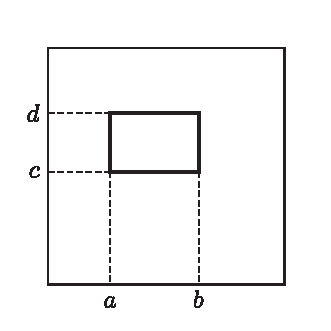
\includegraphics{skript/grafiken/stochastik-1-1-2-a}
\end{center}
$$ p((a, b] \times (c, d]) = (b-a)(d-c) $$
\pagebreak

\paragraph{Achtung:} Der Begriff Gleichverteilung ist nicht bei jeder Objektklasse so leicht zu beschreiben. Zur Veranschaulichung werden zuf�llige Geraden betrachtet, die den Einheitskreis $S$ schneiden, und die L�nge $l$ der Sehne gemessen.
\begin{center}
    \includegraphics{skript/grafiken/stochastik-1-1-2-b}
\end{center}
Das Ereignis $A$ besteht aus allen Geraden, die $S$ schneiden, f�r die gilt, dass $l \geq 1$.
\begin{itemize}
    \item \textbf{1. Ansatz:} \par
    Schnittpunkte von Geraden von $S$ sind gleichverteilt auf $S$. Betrachten nur Geraden durch festen Punkt $P \in S$.
    \begin{center}
        \includegraphics{skript/grafiken/stochastik-1-1-2-c}
    \end{center}
    Geraden durch $P$ sind gleichverteilt bez�glich des Winkels $\alpha$ zur Tangente ($0 \leq \alpha \leq \pi$).
    \begin{eqnarray*}
    l \geq 1 &\Leftrightarrow& \frac{\pi}{6} \leq \alpha \leq \frac{5\pi}{6} \\
    p(A) &=& \frac{\frac{5\pi}{6} - \frac{\pi}{6}}{\pi} = \frac{2}{3} \approx 0,67
    \end{eqnarray*}

    \item \textbf{2. Ansatz:} \par
    Alle Richtungen sind gleichverteilts, deshalb betrahten wir nur Geraden einer bestimmten Richtung, o.B.d.A. nur horizonrale Geraden.
    \begin{center}
        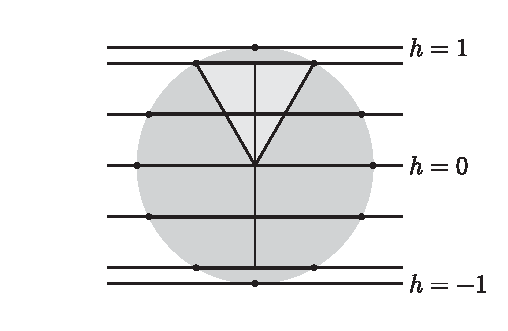
\includegraphics{skript/grafiken/stochastik-1-1-2-d}
    \end{center}
    Geraden sind gleichverteilt bez�glich $-1 \leq h \leq 1$.
    \begin{eqnarray*}
    h^2 + \left( \frac{1}{2} \right)^2 = 1 &\Rightarrow& h = \frac{\sqrt{3}}{2} \\
    p(A) &=& \frac{2 \cdot \frac{\sqrt{3}}{2}}{2} = \frac{\sqrt{3}}{2} \approx 0,87
    \end{eqnarray*}

    \item \textbf{3. Ansatz:} \par
     Jede Gerade ist durch den Mittelpunkt $q$ auf ihrer Sehne bestimmt (au�er Durchmesser: sind vernachl�ssigbar).
    \begin{center}
        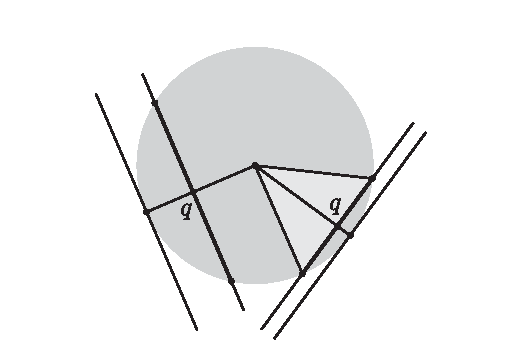
\includegraphics{skript/grafiken/stochastik-1-1-2-e}
    \end{center}
    Annahme: Punkte $q$ sind gleichverteilt auf Kreisscheibe.
    \begin{eqnarray*}
        l \geq 1 &\Leftrightarrow& \text{Abstand von $q$ zu $(0, 0)$} \leq \frac{\sqrt{3}}{2} \\
        p(A) &=& \frac{\text{Fl�che von Kreis mit Radius } \frac{\sqrt{3}}{2}}{\text{Fl�che von Einheitskreis}} = \frac{\pi \cdot \frac{3}{4}}{\pi \cdot 1} = \frac{3}{4}
    \end{eqnarray*}
\end{itemize}

%%%%%%%%%%%%%%%%%%%%%%%%%%%%%%%%%%%%%%%%%%%%%%%%%%%%%%%%%%%%%%%%%%%%%%%%%%%%%%%
\subsection{Bedingte Wahrscheinlichkeit und Unabh�ngigkeit}

\paragraph{Definition:} Sei $(\Omega, \bigF, p)$ ein Wahrscheinlichkeitsraum, die Ereignisse $A, B \in \bigF$ und $p(B) > 0$, so ist die \emph{bedingte Wahrscheinlichkeit}\index{bedingte Wahrscheinlichkeit} von Ereignis $A$ unter $B$ gegeben durch
$$ p(A \, | \,B) = \frac{p(A \cap B)}{p(B)} $$

\paragraph{Beispiel:\;} Sei $\Omega = [0, 1] \times [0, 1]$ eine Menge der Ereignisse mit Gleichverteilung:
\begin{itemize}
    \item $A = \{ (x, y) \; | \; x \geq \frac{1}{3} \}$
    \item $B = \{ (x, y) \; | \; y \geq \frac{1}{3} \}$
    \item $C = \{ (x, y) \; | \; x \leq \frac{2}{3} \}$
\end{itemize}
\begin{center}
        \includegraphics{skript/grafiken/stochastik-1-1-3-a}
\end{center}
\begin{eqnarray*}
  p(A) = p(B) = p(C) &=& \frac{2}{3} \\
  p(A \cap B) &=& \frac{4}{9} \\
  p(A \cap C) &=& \frac{1}{3} \\
  p(A \, | \, B) &=& \frac{\frac{4}{9}}{\frac{2}{3}} = \frac{2}{3} = p(A) \\
  p(A \, | \, C) &=& \frac{\frac{1}{3}}{\frac{2}{3}} = \frac{1}{2} \neq p(A)
\end{eqnarray*}
\pagebreak

\paragraph{Definition:} Zwei Ereignisse $A$ und $B$ sind \emph{unabh�ngig}\index{unabh�ngige Ereginisse}, wenn
$$ p(A \cap B) = p(A) \cdot p(B) $$
\paragraph{Folgerung:} Wenn $A$ und $B$ unabh�ngig und $p(B) > 0$, dann
$$ p(A \, | \, B) = p(A) $$

\paragraph{Definition:} Eine Familie $\{ A_i \; | \; i \in I \}$ von Ereignissen ist unabh�ngig, wenn f�r jede endliche Teilmenge $J \subseteq I$
$$ p \left( \bigcap_{i \in J} A_i \right) = \prod_{i \in J} p(A_i) $$
Achtung:\; Es gibt Familien von paarweise unabh�ngigen Ereignissen, die nicht unabh�ngig sind.

\paragraph{Beispiel:} Sei $\Omega = \{ a, b, c, d \}$ eine Menge der Elementarereignisse mit den Wahrscheinlichkeiten $p(a) = p(b) = p(c) = p(d) = \frac{1}{4}$. Es seien gegeben die folgenden Ereignisse:
\begin{itemize}
    \item $A = \{a, d\}$
    \item $B = \{b, d\}$
    \item $C = \{c, d\}$
\end{itemize}
\begin{eqnarray*}
    p(A) = p(B) = p(C) &=& \frac{1}{2} \\
    p(A \cap B) &=& \frac{1}{4} = p(A) \cdot p(B) \\
    p(A \cap C) &=& \frac{1}{4} = p(A) \cdot p(C) \\
    p(B \cap C) &=& \frac{1}{4} = p(B) \cdot p(C) \\
\end{eqnarray*}
Das hei�t, dass die Ereignisse paarweise unabh�ngig sind. Dennoch ist die Familie mit den Ereignissen $\{A, B, C \}$ \emph{nicht} unabh�ngig:
\begin{eqnarray*}
  p(A \cap B \cap C) = \frac{1}{4} &\neq& \frac{1}{8} = p(A) \cdot p(B) \cdot p(C)
\end{eqnarray*}

\paragraph{Satz (Partitionstheorem):} Sei $\{ B_1, B_2, \ldots \}$ eine Partition von $\Omega$, wobei f�r alle $B_i$ gilt, dass $p(B_i) > 0$. Dann ist
$$ p(A) = \sum_i p(A \, | \, B_i) \cdot p(B_i) \platz \text{f�r alle $A \in \bigF$} $$

\paragraph{Beweis:}
\begin{eqnarray*}
    p(A) &=& p(A \cap \Omega) \\
         &=& p \left( A \cap \left( \bigcup_i B_i \right) \right) \\
         &=& p \left( \bigcup_i \left( A \cap B_i \right) \right) \platz \text{(disjkunte Vereinigung)}\\
         &=& \sum_i p(A \cap B_i) \\
         &=& \sum_i \frac{p(A \cap B_i)}{p(B_i)} \cdot p(B_i) \\
         &=& \sum_i p(A \, | \, B_i) \cdot p(B_i)
\end{eqnarray*}

\paragraph{Beispiel:} Morgen fr�h regnet es ($R$) oder schneit ($S$) oder es gibt keinen Niederschlag ($K$).
\begin{itemize}
    \item Bei Regen ist die Wahrscheinlichkeit f�r eine Busversp�tung $\frac{1}{3}$.
    \item Bei Schnee ist die Wahrscheinlichkeit f�r eine Busversp�tung $\frac{2}{3}$.
    \item Bei Regen ist die Wahrscheinlichkeit f�r eine Busversp�tung $\frac{1}{6}$.
\end{itemize}
Die Wettervorhersage:
\begin{itemize}
    \item $p(R) = \frac{1}{5}$
    \item $p(S) = p(K) = \frac{2}{5}$
\end{itemize}
$$ p(\text{Busversp�tung}) = \frac{1}{3} \cdot \frac{1}{5} + \frac{2}{3} \cdot \frac{2}{5} + \frac{1}{6} \cdot \frac{2}{5} = \frac{2+8+2}{30} = \frac{12}{30} = \frac{2}{5} $$
\pagebreak

%%%%%%%%%%%%%%%%%%%%%%%%%%%%%%%%%%%%%%%%%%%%%%%%%%%%%%%%%%%%%%%%%%%%%%%%%%%%%%%
% Zufallsvariablen
%%%%%%%%%%%%%%%%%%%%%%%%%%%%%%%%%%%%%%%%%%%%%%%%%%%%%%%%%%%%%%%%%%%%%%%%%%%%%%%
\section{Zufallsvariablen}
%%%%%%%%%%%%%%%%%%%%%%%%%%%%%%%%%%%%%%%%%%%%%%%%%%%%%%%%%%%%%%%%%%%%%%%%%%%%%%%
\subsection{Diskrete Zufallsvariablen}

\paragraph{Definition:} Sei $(\Omega, \bigF, p)$ ein Wahrscheinlichkeitsraum. Eine Funktion
$$ X : \Omega \rightarrow \real $$
ist eine \emph{diskrete Zufallsvariable}\index{Zufallsvariable, diskret}\index{diskrete Zufallsvariable}, falls
\begin{itemize}
    \item das Bild der Zufallsvariable
    $$ \text{Im} \; X = \{ x \in \real \; | \; \exists \; \omega \in \Omega \platz x = X(\omega) \} $$
    abz�hlbar ist und
    \item f�r alle $x \in \real$:
    $$ X^{-1}(x) = \{ \omega \; | \; X(\omega) = x \} \in \bigF $$
\end{itemize}

\paragraph{Konsequenz:} F�r alle $T \subseteq \real$ ist
$$ X^{-1}(T) \in \bigF $$
denn
$$ X^{-1}(T) = \bigcup_{x \in (T \; \cap \; \text{Im} \; X)} X^{-1}(x) $$

\paragraph{Definition:} Sei $X$ eine diskrete Zufallsvariable auf $(\Omega, \bigF, p)$. Die \emph{Gewichtsfunktion}\index{Gewichtsfunktion} $p_X : \real \rightarrow [0, 1]$ von $X$ sei wie folgt definiert:
$$ p_X(x) = p(X^{-1}(x)) $$
Oft verwendet man f�r $p_X(x)$ auch die intuitivere Schreibweise $p(X = x)$.

\paragraph{Konsequenz:}
\begin{eqnarray*}
    \sum_{x \in \text{Im} \; X} p_X(x) &=& \sum_{x \in \text{Im} \; X} p(\{ \omega \; | \; X(\omega) = x \}) \\
                                       &=& p \left( \bigcup_{x \in \text{Im} \; X} \{ \omega \; | \; X(\omega) = x \} \right) \\ \\
                                       &=& p(\Omega) = 1
\end{eqnarray*}
Die Funktion $p_X$ charakterisiert die Zufallsvariable $X$ sehr genau, in dem Sinne, dass man f�r jede solche Beschreibung eine Realisierung durch einen Wahrscheinlichkeitsraum und eine Zufallsvariable finden kann. \par \vspace{0.3cm} \pagebreak

Sei $S \subseteq \real$ abz�hlbar und f�r jedes $s \in S$ sei eine Zahl $\pi_s \in [ \, 0, 1 \, ]$ gegeben mit
$$ \sum_{s \in S} \pi_s = 1 $$
Konstruktion:
\begin{itemize}
    \item $\Omega = S$
    \item $\bigF = \pot(S)$
    \item $p(A) = \underset{s \in A}{\sum} \pi_s$ f�r jedes $A \subseteq S$
    \item $X: \Omega \rightarrow \real$
    \item $X(s) = s$
\end{itemize}

\paragraph{Beispiele:} $p$ ohne Zusatz ist eine Zahl aus $[ \, 0, 1 \, ]$, $q = 1 - p$
\begin{enumerate}
    \item \emph{Bernoulli-Verteilung}\index{Bernoulli-Verteilung}: \\
    Eine Zufallsvariable $X$ mit Bernoulli-Verteilung:
    \begin{itemize}
        \item $\text{Im} \; X = \{ 0, 1 \}$
        \item $p_X(0) = q \platz \text{und} \platz p_X(1) = p$
    \end{itemize}
    Probe: $p_X(0) + p_X(1) = p + q = p + (1 - q) = 1$ \par
    z.B. M�nzwurf mit "`unfairer"' M�nze:
    \begin{itemize}
        \item Wahrscheinlichkeit f�r Kopf $K$: $p$
        \item Wahrscheinlichkeit f�r Zahl $Z$: $q = 1 - p$
    \end{itemize}
    Die Zufallsvariable wird folgenderma�en definiert:
    \begin{eqnarray*}
        X &:& \{ \text{K}, \text{Z} \} \rightarrow \{ 0, 1 \} \\
        X(K) &=& 1 \\
        X(Z) &=& 0
    \end{eqnarray*}
    \item \emph{Binominialverteilung}\index{Binominialverteilung} \\
    Eine Zufallsvariable $X$ mit Binominialverteilung mit den Parametern $n$~und~$p$:
    \begin{itemize}
        \item $\text{Im} \; X = \{ 0, 1, \ldots, n \}$ und
        \item $p_X(k) = \left( {n \atop k} \right) \; p^k \; q^{n-k}$ f�r alle $k \in \{ 0, 1, \ldots, n \}$
    \end{itemize}
    Probe: $ \underset{k=0}{\overset{n}{\sum}} p_X(k) = \underset{k=0}{\overset{n}{\sum}} \left( { n \atop k } \right) \; p^k \; q^{n-k} = (p + q)^n = 1^n = 1 $ \par
    Binominialverteilung tritt auf z.B. bei $n$-facher Wiederholung eines Bernoulli-Experiments (unabh�ngig).
    \begin{itemize}
        \item $\Omega = \{ \text{K}, \text{Z} \}^n$
        \item $\omega = (a_1, a_2, \ldots, a_n)$ mit $a_i = \{ \text{K}, \text{Z} \}$
        \item $p(\omega) = p^{k(\omega)} \cdot q^{z(\omega)}$
        \item $X(\omega) := k(\omega)$
    \end{itemize}
    mit $k(\omega) = $ Anzahl der K�pfe in $\omega$ und $z(\omega) = $ Anzahl der Zahlen in $\omega$ \par \vspace{0.3cm}
    Wahrscheinlichkeit, dass bei $n$ M�nzw�rfen genau $k$-mal Kopf f�llt:
    \begin{eqnarray*}
        p_X(k) &=& p(\{ \omega \; | \; X(\omega) = k \}) \\
               &=& p(\{ \omega \; | \; k(\omega) = k \}) \\
               &=& \sum_{\omega \text{ mit} \atop k(w) = k} p(\omega) \\
               &=& \sum_{\omega \text{ mit} \atop k(w) = k} p^{k} \; q^{n-k} \\
               &=& \left( { n \atop k } \right) \; p^k \; q^{n-k}
    \end{eqnarray*}
    \item \emph{Geometrische Verteilung}\index{geometrische Verteilung}: \\
    Wiederholung eines Wurfes einer $(p, q)$-M�nze so lange, bis zum erstem mal K auftritt:
    \begin{itemize}
        \item $\Omega = \{ \text{K}, \text{ZK}, \text{ZZK}, \text{ZZZK}, \text{ZZZZK}, \ldots \}$
        \item $p((\text{K})) = p$, $p((\text{ZK}) = qp$, $p((\text{Z}^l \text{K})) = q^l \; p$
        \item $X(\omega) = |\omega|$ (Anzahl der W�rfe)
        \item $\text{Im}(X) = \{ 1, 2, 3, \ldots \}$
        \item $p_X(k) = p(\{ \omega \; | \; |\omega| = k \}) = p(\text{Z}^{k-1} K) = q^{k-1} \cdot p$
    \end{itemize}
    \item \emph{Poisson-Verteilung}\index{Poisson-Verteilung}: \\
    Eine Zufallsvariable $X$ mit Poisson-Verteilung mit Parameter $\lambda$:
    \begin{itemize}
        \item $\text{Im}(X) = \nat$ \platz (inkl. der Null)
        \item $p_X(k) = \frac{1}{k!} \; \lambda^k \; e^{- \lambda}$
    \end{itemize}
    Probe: $\underset{k=0}{\overset{\infty}{\sum}} p_X(k) = \underset{k=0}{\overset{\infty}{\sum}} \frac{1}{k!} \; \lambda^k \; e^{- \lambda} = e^{- \lambda} \cdot \sum_{k=0}^{\infty} \frac{1}{k!} \; \lambda^k = e^{- \lambda} \cdot e^{\lambda} = 1$ \par
    Die Poisson-Verteilung tritt auf als Grenzwert von Binominialverteilung mit $n$ gro�, $p$ klein, $\lambda = n \cdot p$ und $k \ll n$.
    \begin{eqnarray*}
        \left( { n \atop k } \right) \cdot p^k \cdot (1-p)^{n-k} &=& \left( { n \atop k } \right) \; \left( \frac{\lambda}{n} \right)^k \; (1-p)^{n-k} \\
                                                                 &\approx& \frac{n^k}{k!} \cdot \frac{\lambda^k}{n^k} \cdot \left( 1 - \frac{\lambda}{n} \right)^n \cdot \left( 1 - \frac{\lambda}{n} \right)^{-k} \\
                                                                 &\approx& \frac{\lambda^k}{k!} \cdot e^{- \lambda}
    \end{eqnarray*}
\end{enumerate}

%%%%%%%%%%%%%%%%%%%%%%%%%%%%%%%%%%%%%%%%%%%%%%%%%%%%%%%%%%%%%%%%%%%%%%%%%%%%%%%
\subsection{Stetige Zufallsvariablen}

\paragraph{Definition:} Eine \emph{Zufallsvariable}\index{Zufallsvariable} auf $(\Omega, \bigF, p)$ ist eine Abbildung $X : \Omega \rightarrow \real$, so dass f�r alle $x \in \real$ gilt:
$$ \{ \omega \in \Omega \; | \; X(\omega) \leq x \} \in \bigF $$
\paragraph{Definition:} Die Funktion
$$ F_X(x) = p(\{ \omega \in \Omega \; | \; X(\omega) \leq x \}) $$
nennt man die \emph{Verteilungsfunktion}\index{Verteilungsfunktion} von $X$.

\paragraph{Lemma:} F�r jede Verteilungsfunktion $F = F_X$ einer Variablen $X : \Omega \rightarrow \real$ gilt:
\begin{enumerate} \buchstaben
    \item $x \leq y \platz \Rightarrow \platz F(x) \leq F(y)$
    \item $\underset{x \to - \infty}{\lim} F(x) = 0$ und $\underset{x \to \infty}{\lim} F(x) = 1$
    \item $\forall \; x \in \real \platz \underset{h \to 0+}{\lim} F(x+h) = F(x)$
\end{enumerate}

\paragraph{Beweis:} Sei $A_x = \{ \omega \in \Omega \; | \; X(\omega) \leq x \} \in \bigF$ und $F(x) = p(A_x)$
\begin{enumerate} \buchstaben
    \item $x \leq y \platz \Rightarrow \platz A_x \subseteq A_y \platz \Rightarrow \platz \underbrace{p(A_x)}_{F(x)} \leq \underbrace{p(A_y)}_{F(y)}$
    \item $\emptyset = \underset{x=1}{\overset{\infty}{\bigcap}} A_{-x} \platz \Rightarrow \platz 0 = p(\emptyset) = \underset{x \to \infty}{\lim} p(A_{-x}) = \underset{x \to - \infty}{\lim} F(x)$ \par
          $\Omega = \underset{x=1}{\overset{\infty}{\bigcup}} A_x \platz \Rightarrow \platz 1 = p(\Omega) = \underset{x \to \infty}{\lim} p(A_n) = \underset{x \to \infty}{\lim} F(x)$
\end{enumerate}

\paragraph{Achtung:} Die Funktion $F_X$ ist nicht zwingend stetig, z.B. bei geometrischer Verteilung:
\begin{center}
    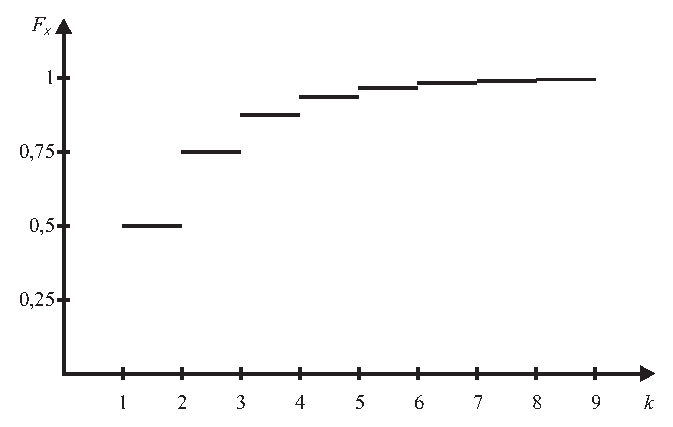
\includegraphics{skript/grafiken/stochastik-1-2-2-a}
\end{center}

\paragraph{Definition:} Eine Zufallsvariable $X : \Omega \rightarrow \real$ ist \emph{stetig}\index{stetige Zufallsvariable}\index{Zufallsvariable, stetig}, wenn eine Funktion $f: \real \to \real^+$ existiert, so dass
$$ F_X(x) = \int_{\infty}^{x} f(n) \; dn $$
$f$ wird \emph{Dichte}\index{Dichte} der Verteilung genannt.

\paragraph{Beispiel:} Gleichverteilung im Intervall $[ \, 1, 3 \, ]$. \par \vspace{0.3cm}
Ist $1 \leq y \leq x \leq 3$, so ist
$$ p(\{ \omega \; | \; \omega \in [ \, y, x \, ] \}) = \frac{x-y}{3-1} $$
$X$ hat die Verteilung
$$ F_X(x) = p(\{ \omega \; | \; X(\omega) \leq x \}) = \frac{x-1}{3-1} = \frac{x-1}{2} $$ \pagebreak

Suche $f$, so dass
$$ F_X(x) = \int_{- \infty}^{\infty} f(n) \; dn $$
\begin{center}
    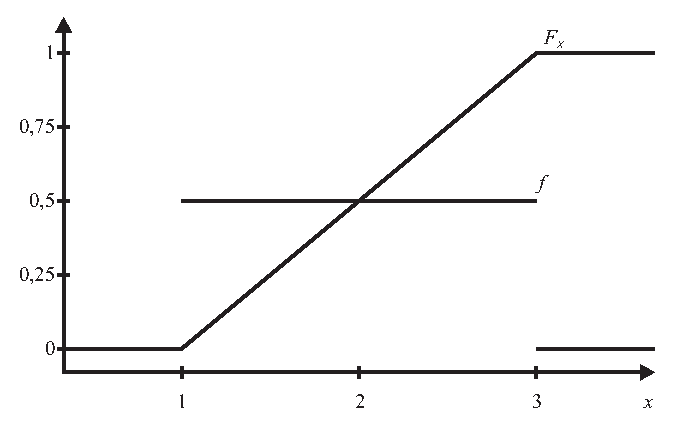
\includegraphics{skript/grafiken/stochastik-1-2-2-b}
\end{center}
Gesuchte Funktion lautet:
$$ f(x) = \left\{ \begin{array}{lll}
  \frac{1}{2} & \text{ falls } & x \in [ \, 1, 3 \, ] \\ \\
  0           & \text{ sonst}
\end{array} \right.$$

\paragraph{Vergleich:}
\begin{itemize}
    \item diskret
    \begin{itemize}
        \item Gewichtsfunktion $p_X$
        \item Addition der Einzelwahrscheinlichkeiten
    \end{itemize}
    \item stetig
    \begin{itemize}
        \item Dichtefunktion $f$
        \item Integrieren �ber der Dichtefunktion
    \end{itemize}
\end{itemize} \pagebreak

%%%%%%%%%%%%%%%%%%%%%%%%%%%%%%%%%%%%%%%%%%%%%%%%%%%%%%%%%%%%%%%%%%%%%%%%%%%%%%%
% Erwartungswert
%%%%%%%%%%%%%%%%%%%%%%%%%%%%%%%%%%%%%%%%%%%%%%%%%%%%%%%%%%%%%%%%%%%%%%%%%%%%%%%
\section{Erwartungswert}
%%%%%%%%%%%%%%%%%%%%%%%%%%%%%%%%%%%%%%%%%%%%%%%%%%%%%%%%%%%%%%%%%%%%%%%%%%%%%%%
\subsection{Bestimmung des Erwartungswertes}

\paragraph{Definition:} Ist $X : \Omega \rightarrow \real$ eine diskrete Zufallsvariable, so ist der der \emph{Erwartungswert}\index{Erwartungswert} von $X$ definiert durch
$$ E(X) = \sum_{x \in \text{Im} X} x \cdot p_X(x) = \sum_{x \in \text{Im} X} x \cdot p(\{ \omega \; | \; X(\omega) = x \}) $$
falls diese Reihe absolut konvergiert.

\paragraph{Definition:} Ist $X : \Omega \rightarrow \real$ eine stetige Zufallsvariable mit der Dichtefunktion~$f$, so ist
$$ E(X) = \int_{\infty}^{\infty} x \cdot f(x) dx $$
falls beide uneigentlichen Integrale existieren.

\paragraph{Lemma (Linearit�t der Erwartungswerte):} Sind $X$ und $Y$ Zufallsvariablen �ber $(\Omega, \bigF, p)$ mit den Erwartungswerten $E(X)$ und $E(Y)$, dann gilt:
\begin{itemize}
    \item $E(X + Y) = E(X) + E(Y)$ \\
    mit $(X + Y)(\omega) = X(\omega) + Y(\omega)$
    \item $E(\alpha \cdot X) = \alpha \cdot E(X)$ \\
    mit $(\alpha \cdot X)(\omega) = \alpha \cdot X(\omega)$ und $\alpha \in \real$
\end{itemize}

\paragraph{Beispiele:}
\begin{enumerate}
    \item Zufallsvariable $X$ mit Bernoulli-Verteilung mit Parameter $p$:
    \begin{itemize}
        \item $\text{Im} X = \{ 0, 1 \}$
        \item $p_X(1) = p$ und $p_X(0) = 1 - p$
        \item $E(X) = 1 \cdot p + 0 \cdot (1 - p) = p$
    \end{itemize}

    \item Zufallsvariable $X$ mit Binominialverteilung mit den Parametern $n$ und $p$:
    \begin{itemize}
        \item $X = X_1 + X_2 + X_3 + \ldots X_n$ \platz mit $X_i = \left\{ \begin{array}{ll} 1 & \text{ falls $i$-ter Wurf $K$ ist} \\ 0 & \text{ falls $i$-ter Wurf $Z$ ist} \end{array} \right.$
        \item $E(X_i) = p$
        \item $E(X) = E(X_1) + E(X_2) + E(X_3) + \ldots + E(X_n) = n \cdot p$
    \end{itemize} \pagebreak[2]

    \item Zufallsvariable $X$ mit geometrischer Verteilung mit Parameter $p$:
    \begin{itemize}
        \item $\text{Im} X = \nat^+$
        \item $p_X(k) = (1 - p)^{k-1} \cdot p = q^{k-1} \cdot p$
    \end{itemize}
    Bestimmung des Erwartungswertes:
    \begin{eqnarray*}
        E(X) &=& \sum_{k=1}^{\infty} k \cdot (1 - p)^{k-1} \cdot p \\
             &=& p \cdot \left( \sum_{k=1}^{\infty} q^{k-1} + \sum_{k=2}^{\infty} q^{k-1} + \sum_{k=3}^{\infty} q^{k-1} + \ldots \right) \\
             &=& p \cdot \left( \sum_{k=0}^{\infty} q^k + q \cdot \sum_{k=0}^{\infty} q^k + q^2 \cdot \sum_{k=0}^{\infty} q^k + \ldots \right) \\
             &=& p \cdot \left( \frac{1}{1-q} + \frac{q}{1-q} + \frac{q^2}{1-q} + \ldots \right) \\
             &=& \frac{p}{1-q} \cdot \left( 1 + q + q^2 + \ldots \right) \\
             &=& 1 \cdot \frac{1}{1-q} \\
             &=& \frac{1}{p}
    \end{eqnarray*}

    \item Zufallsvariable $X$ mit Poisson-Verteilung mit Paramter $\lambda$:
    \begin{itemize}
        \item $\text{Im} X = \nat$
        \item $p_X(k) = \frac{1}{k!} \cdot \lambda^k \cdot e^{- \lambda}$
    \end{itemize}
    Bestimmung des Erwartungswertes:
    \begin{eqnarray*}
        E(X) &=& \sum_{k=0}^{\infty} k \cdot \frac{1}{k!} \cdot \lambda^k \cdot e^{- \lambda} \\
             &=& \sum_{k=1}^{\infty} k \cdot \frac{1}{(k-1)!} \cdot \lambda^k \cdot e^{- \lambda} \\
             &=& \lambda \cdot \sum_{k=1}^{\infty} k \cdot \frac{1}{(k-1)!} \cdot \lambda^{k-1} \cdot e^{- \lambda} \\
             &=& \lambda
    \end{eqnarray*}

    \item stetige Zufallsvariable $X$ mit Gleichverteilung �ber einem Intervall $[ \, a, b \, ]$:
    \begin{eqnarray*}
        E(X) &=& \int_{\infty}^{\infty} x \cdot f(x) dx \\
             &=& \int_a^b x \cdot \frac{1}{b-a} \; dx \\
             &=& \frac{1}{b-a} \cdot \int_a^b x \; dx \\
             &=& \frac{1}{b-a} \cdot \left[ \frac{1}{2} \; x^2 \right]_a^b \\
             &=& \frac{1}{b-a} \cdot \left( \frac{1}{2} \; b^2 - \frac{1}{2} \; a^2 \right) \\
             &=& \frac{b^2 - a^2}{2(b-a)} \\
             &=& \frac{(b+a)(b-a)}{2(b-a)} \\
             &=& \frac{a+b}{2}
    \end{eqnarray*}
\end{enumerate}

%%%%%%%%%%%%%%%%%%%%%%%%%%%%%%%%%%%%%%%%%%%%%%%%%%%%%%%%%%%%%%%%%%%%%%%%%%%%%%%
\subsection{Abweichungen vom Erwartungswert}

\paragraph{Satz (Markow-Ungleichung):} Sei $X : \Omega \rightarrow \real^{\geq 0}$ eine Zufallsvariable mit dem Erwartungswert $E(X)$ unt $t > 0$, dann gilt:
$$ p(X \geq t) \leq \frac{E(X)}{t} $$

\paragraph{Beweis f�r diskrete Variablen:}
\begin{eqnarray*}
    E(X) &=& \sum_{x \in \text{Im} X} x \cdot p(X = x) \\
         &=& \sum_{x \in \text{Im} X \atop x < t} x \cdot p(X = x) + \sum_{x \in \text{Im} X \atop x \geq t} x \cdot p(X = x) \\
         &\geq& \sum_{x \in \text{Im} X \atop x \geq t} x \cdot p(X = x) \\
         &\geq& t \cdot \sum_{x \in \text{Im} X \atop x \geq t} p(X = x) \\
         &=& t \cdot p(X \geq t) \\ \\
    \frac{E(X)}{t} &\geq& p(X \geq t)
\end{eqnarray*}

\paragraph{Satz:} Sei $X : \Omega \rightarrow \real$ eine diskrete Zufallsvariable und $g : \real \rightarrow \real$ eine beliebige Funktion, dann ist $Y = gX : \Omega \rightarrow \Omega$ eine Zufallsvariable mit
$$ Y(\omega) = g(X(\omega)) $$
und
$$ E(Y) = \sum_{x \in \text{Im} X} g(x) \cdot p_X(x) $$
falls diese Reihe absolut konvergiert.

\paragraph{Beispiel:} Sei $X$ eine Zufallsvariable mit geometrischer Verteilung mit dem Parametern $p$ und $g(x) = x^2$ eine Funktion ($q = 1 - p$):
\begin{eqnarray*}
    E(gX) &=& E(X^2) \\ \\
          &=& \sum_{k=1}^{\infty} k^2 \cdot q^{k-1} \cdot p \\ \\
          &=& \sum_{k=1}^{\infty} 1^2 \cdot q^{k-1} \cdot p + \sum_{k=2}^{\infty} \underbrace{(2^2 - 1^2)}_{(2+1)(2-1)} \cdot q^{k-1} \cdot p + \sum_{k=1}^{\infty} \underbrace{(3^2 - 2^2)}_{(3+2)(3-2)} \cdot q^{k-1} \cdot p + \ldots \\ \\
          &=& 1 + (1+2) \cdot q \cdot \underbrace{\sum_{k=1}^{\infty} p \cdot q^{k-1}}_{1} + (1+4) \cdot q^2 \cdot \underbrace{\sum_{k=1}^{\infty} p \cdot q^{k-1}}_{1} + (1+6) \cdot q^3 \cdot \ldots \\ \\
          &=& 1 + q + q^2 + q^3 + \ldots + 2 \cdot q + 4 \cdot q^2 + 6 \cdot q^3 + \ldots \\ \\
          &=& \frac{1}{1-q} + \frac{2q}{p^2} \cdot \sum_{k=0}^{\infty} k \cdot q^k \cdot p \\ \\
          &=& \frac{1}{p} + \frac{2q}{p^2} \\ \\
          &=& \frac{p+2-2p}{p^2} \\ \\
          &=& \frac{2-p}{p^2} \\
\end{eqnarray*}

\paragraph{Definition:} Die Erwartungswerte $E(X^i)$ werden $i$-tes \emph{Moment}\index{Moment} von $X$ genannt.

\paragraph{Definition:} Die \emph{Varianz}\index{Varianz} einer Zufallsvariable $X$ mit $E(X) = \mu$ ist
\begin{eqnarray*}
    \text{\emph{Var}}(X) &=& E((X - \mu)^2) \\
                         &=& E((X - E(X))^2) \\
                         &=& E \left( X^2 - 2 \cdot X \cdot E(X) + (E(X))^2 \right) \\
                         &=& E(X^2) - 2 \cdot E(X) \cdot E(X) + (E(X))^2 \\
                         &=& E(X^2) - 2 \cdot (E(X))^2 + (E(X))^2 \\
                         &=& \underbrace{E(X^2)}_{\text{2. Moment}} - \underbrace{(E(X))^2}_{(\text{1. Moment})^2}
\end{eqnarray*}
Die Gr��e $\sigma = \sqrt{\text{\emph{Var}}(X)}$ wird \emph{Standardabweichung}\index{Standardabweichung} von $X$ genannt.

\paragraph{Beispiele:}
\begin{enumerate}
    \item Zufallsvariable $X$ mit Bernoulli-Verteilung mit Parameter $p$:
    \begin{eqnarray*}
        \text{\emph{Var}}(X) &=& E(X^2) - (E(X))^2 \\
                             &=& (1^2 \cdot p + 0^2 \cdot (1-p)) - (1 \cdot p + 0 \cdot (1-p))^2 \\
                             &=& p - p^2
    \end{eqnarray*}
    \item Zufallsvariable $X$ mit Binominialverteilung mit den Parametern $n$ und $p$: \par
    An der Stelle kann genutzt werden, dass f�r \emph{unabh�ngige} Zufallsvariablen gilt:
    \begin{itemize}
        \item $\text{\emph{Var}}(X+Y) = \text{\emph{Var}}(X) + \text{\emph{Var}}(Y)$
        \item $p(X=x \land Y=y) = p(X=x) \cdot p(Y=y)$
    \end{itemize}
    Eine Zufallsvariable $X$ mit Binominialverteilung ist eine Summe aus unabh�ngigen Bernoulli-Variablen:
    \begin{eqnarray*}
        X &=& X_1 + X_2 + \ldots + X_n
    \end{eqnarray*}
    Damit ergibt sich f�r die Varianz:
    \begin{eqnarray*}
        \text{\emph{Var}}(X) &=& n \cdot (p - p^2)
    \end{eqnarray*}
    \item Zufallsvariable $X$ mit geometrischer Verteilung mit Parameter $p$:
    \begin{eqnarray*}
        \text{\emph{Var}}(X) &=& E(X^2) - (E(X))^2 \\
                             &=& \frac{2-p}{p^2} - \left( \frac{1}{p} \right)^2 \\
                             &=& \frac{1-p}{p^2} \\
                             &=& \frac{1}{p^2} - \frac{1}{p}
    \end{eqnarray*}
\end{enumerate}

\paragraph{Satz (Tschebyscheff-Ungleichung):} Sei $X$ eine Zufallsvariable mit dem Erwartungswert $E(X) = \mu$ und der Varianz $\text{\emph{Var}}(X) = \sigma^2$, dann gilt f�r alle $c > 0$:
\begin{eqnarray*}
    p(|X - \mu| \geq c) &\leq& \frac{\sigma^2}{c^2}
\end{eqnarray*}
Spezialfall f�r $E(X) = \mu = 0$:
\begin{eqnarray*}
    p(|X| \geq c) &\leq& \frac{E(X^2)}{c^2}
\end{eqnarray*}

\paragraph{Beispiel:} Zufallsvariable $X$ mit Binominialverteilung mit den Parametern $n$ und $p = \frac{1}{2}$:
\begin{eqnarray*}
    E(X) &=& n \cdot \frac{1}{2} = \frac{n}{2} \\
    \text{\emph{Var}}(X) &=& n \cdot \left( \frac{1}{2} - \left( \frac{1}{2} \right)^2 \right) = \frac{n}{4} = \sigma^2 \\
    \text{W�hle: } c &=& \frac{n}{4} \\ \\
    p\left( \left| X - \frac{n}{2} \right| \geq \frac{n}{4} \right) &\leq& \frac{\frac{n}{4}}{\left( \frac{n}{4} \right)^2} = \frac{4}{n} \\ \\
    \lim_{n \to \infty} \frac{4}{n} &=& 0
\end{eqnarray*}
Das hei�t, dass die Wahrscheinlichkeit daf�r, dass bei $n$ W�rfen weniger als $\frac{1}{4}$ oder mehr als $\frac{3}{4}$ der Ergebnisse K�pfe sind, geht f�r gro�e $n$ gegen $0$. \par \vspace{0.3cm}

Dagegen die Absch�tzung mit der Markow-Ungleichung:
\begin{eqnarray*}
    p \left( X \geq \frac{3}{4} \cdot n \right) &\leq& \frac{\frac{n}{2}}{\frac{3}{4} \cdot n} = \frac{2}{3}
\end{eqnarray*} \pagebreak

\paragraph{Gaus'sche Normalverteilung:}\index{Gaus'sche Normalverteilung} $N(\mu, \sigma^2)$ mit Dichtefunktion $f$
$$ f(x) = \frac{1}{\sqrt{2 \pi \sigma^2}} \cdot e^{- \frac{1}{2 \sigma^2} \cdot (x - \mu)^2} $$
\begin{center}
    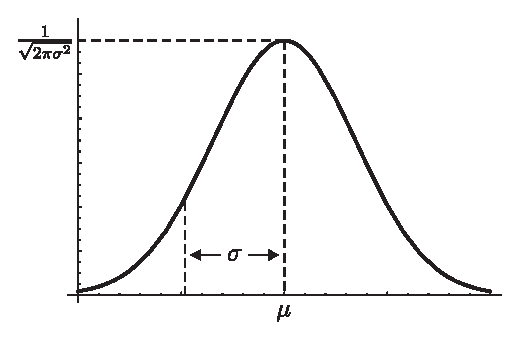
\includegraphics{skript/grafiken/stochastik-1-3-2-b}
\end{center}
Hinweis: Der Abstand von $\mu$ zum Wendepunkt von $f(x)$ betr�gt $\sigma$.

\chapter{Lineare Algebra}

%%%%%%%%%%%%%%%%%%%%%%%%%%%%%%%%%%%%%%%%%%%%%%%%%%%%%%%%%%%%%%%%%%%%%%%%%%%%%%%
% Vektoren - der intuitive Ansatz
%%%%%%%%%%%%%%%%%%%%%%%%%%%%%%%%%%%%%%%%%%%%%%%%%%%%%%%%%%%%%%%%%%%%%%%%%%%%%%%
\section{Vektoren -- der intuitive Ansatz}
%%%%%%%%%%%%%%%%%%%%%%%%%%%%%%%%%%%%%%%%%%%%%%%%%%%%%%%%%%%%%%%%%%%%%%%%%%%%%%%
\subsection{Koordinatenfreie Einf�hrung}

\paragraph{Definition:} Ein \emph{Vektor}\index{Vektor, intuitiv} wird durch geordnetes Punktepaar $\overrightarrow{AB}$ repr�sentiert (veranschaulicht durch die gerichtete Strecke von $A$ nach $B$), wobei zwei Vektoren $\overrightarrow{AB}$ und $\overrightarrow{A'B'}$ gleich sind, wenn es eine Translation (Parallelverschiebung) gibt, die $A$ in $A'$ und $B$ in $B'$ �berf�hrt.
\begin{center}
    \includegraphics{skript/grafiken/lineare-algebra-2-1-1-a}
\end{center}
Zur Betonung des Aspekts, dass der Anfangspunkt beliebig sein kann, wird der Begriff des \emph{freien Vektors}\index{freier Vektor}\index{Vektor, frei} verwendet. \par \vspace{0.3cm}
Legt man einen Bezugspunkt $O$ im Raum fest und betrachtet f�r einen beliebigen Punkt $P$ den Vektor $\overrightarrow{OP}$, so wird dieser der \emph{Ortsvektor}\index{Ortsvektor} von $P$ genannt. \pagebreak

\paragraph{Addition von Vektoren\index{Addition von Vektoren, intuitiv}:} Vertoren werden durch Aneinanderkettung addiert.
\begin{center}
    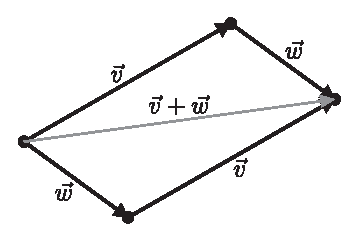
\includegraphics{skript/grafiken/lineare-algebra-2-1-1-b}
\end{center}
Kommutativit�t kann man durch Parallelogrammeigenschaften sehen.

\paragraph{Nullvektor\index{Nullvektor}:} Der Vektor $\overrightarrow{OO} = \overrightarrow{AA}$ wird Nullvektor genannt und kurz mit~$\vec{0}$~bezeichnet. Der Nullvektor ist das neutrale Element der Addition:
$$ \vec{v} + \vec{0} = \vec{v} $$

\paragraph{Inverser Vektor\index{inverser Vektor}:} Der Vektor $\overrightarrow{BA}$ wird als zu $\overrightarrow{AB}$ invers bezeichnet:
$$ \overrightarrow{AB} + \overrightarrow{BA} = \overrightarrow{AA} = \vec{0} $$

\paragraph{Betrag\index{Betrag eines Vektors}:} Der Betrag (L�nge, Norm) des Vektors $\overrightarrow{AB}$ ist der Abstand zwischen $A$ und $B$ und wird mit $\left\| \overrightarrow{AB} \right\|$ bezeichnet. \par \vspace{0.3cm}

\paragraph{Multiplikation mit Skalaren\index{Multiplikation mit Skalaren}:}
\begin{center}
    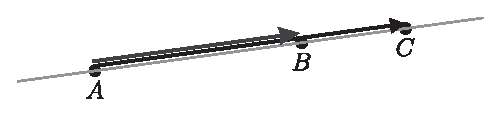
\includegraphics{skript/grafiken/lineare-algebra-2-1-1-c}
\end{center}
Liegen drei Punkte $A$, $B$ und $C$ in dieser Reihefolge auf einer Geraden und ist
$$ \left\| \overrightarrow{AB} \right\| = \lambda \cdot \left\| \overrightarrow{AC} \right\| $$
so sagt man
$$ \overrightarrow{AB} = \lambda \cdot \overrightarrow{AC} $$
Auf diese Weise wird Multiplikation von reellen Zahlen (Skalaren) mit Vektoren eingef�hrt.

%%%%%%%%%%%%%%%%%%%%%%%%%%%%%%%%%%%%%%%%%%%%%%%%%%%%%%%%%%%%%%%%%%%%%%%%%%%%%%%
\subsection{Koordinatensystem}\index{Koordinatensystem}

Betrachtet man zus�tzlich ein Koordinatensystem im Raum mit dem Ursprung $O = (0, 0, 0)$, so kann jedem Punkt $P = (p_1, p_2, p_3)$ der Ortsvektor
$$ \overrightarrow{OP} = \vecthree{p_1}{p_2}{p_3} $$
zugeordnet werden.

\paragraph{Kosequenz:} Aus $P = (p_1, p_2, p_3)$ und $Q = (q_1, q_2, q_3)$ folgt:
$$ \overrightarrow{PQ} = \vecthree{q_1 - p_1}{q_2 - p_2}{q_3 - p_3} $$
\begin{center}
    \includegraphics{skript/grafiken/lineare-algebra-2-1-2-a}
\end{center}

\paragraph{Addition:}
$$ \vecthree{x_1}{x_2}{x_3} + \vecthree{y_1}{y_2}{y_3} = \vecthree{x_1 + y_1}{x_2 + y_2}{x_3 + y_3} $$

\paragraph{Multiplikation mit Skalaren:}
$$ \lambda \cdot \vecthree{x_1}{x_2}{x_3} = \vecthree{\lambda \cdot x_1}{\lambda \cdot x_2}{\lambda \cdot x_3} $$ \pagebreak

\paragraph{Betrag:}
$$ \vec{v} = \vecthree{x}{y}{z} \platz \Rightarrow \platz \left\| \vec{v} \right\| = \sqrt{x^2 + y^2 + z^2} $$
\begin{center}
    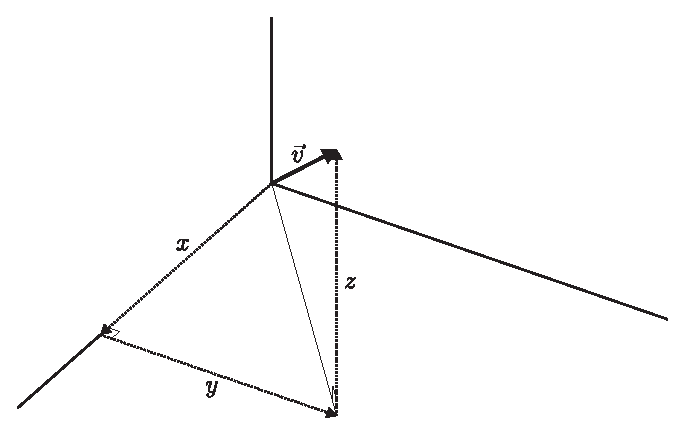
\includegraphics{skript/grafiken/lineare-algebra-2-1-2-b}
\end{center}

\paragraph{Fazit:} Man kann Vektoren im Raum genauso darstellen wie Punkte, aber im Gegensatz zu Punkten k�nnen Vektoren addiert und mit Skalaren multipliziert werden.

%%%%%%%%%%%%%%%%%%%%%%%%%%%%%%%%%%%%%%%%%%%%%%%%%%%%%%%%%%%%%%%%%%%%%%%%%%%%%%%
\subsection{Zusammenhang zwischen Vektoren und linearen Gleichungssystemen (LGS)}

\paragraph{Beispiel:} Die folgenden Probleme sind �quivalent:
\begin{itemize}
    \item Hat dieses lineare Gleichungssystem eine L�sung?
    $$ \begin{array}{ccccc}
    5 \alpha & + & 3 \beta & = & -1 \\
    4 \alpha & + & \beta & = & 2 \\
    3 \alpha & - & \beta & = & 5 \\
    \end{array} $$
    \item Gibt es entsprechende $\alpha$ und $\beta$?
    $$ \alpha \begin{pmatrix} 5 \\ 4 \\ 3 \end{pmatrix} + \beta \begin{pmatrix} 3 \\ 1 \\ -1 \end{pmatrix} = \begin{pmatrix} -1 \\ 2 \\ 5 \end{pmatrix} $$
    \item Liegt der Punkt $(-1, 2, 5)$ in der Ebene, die von den Punkten $(0, 0, 0)$, $(5, 4, 3)$ und $(3, 1, -1)$ aufgespannt wird?
\end{itemize}


%%%%%%%%%%%%%%%%%%%%%%%%%%%%%%%%%%%%%%%%%%%%%%%%%%%%%%%%%%%%%%%%%%%%%%%%%%%%%%%
% Vektorr�ume
%%%%%%%%%%%%%%%%%%%%%%%%%%%%%%%%%%%%%%%%%%%%%%%%%%%%%%%%%%%%%%%%%%%%%%%%%%%%%%%
\section{Vektorr�ume}
%%%%%%%%%%%%%%%%%%%%%%%%%%%%%%%%%%%%%%%%%%%%%%%%%%%%%%%%%%%%%%%%%%%%%%%%%%%%%%%
\subsection{Vektorr�ume}

\paragraph{Definition:} Eine Menge $K$ mit zwei Operationen $\oplus$ und $\odot$ und zwei Elementen~$0$ und $1$ (wobei $0 \neq 1$) ist ein \emph{K�rper}\index{K�rper}, falls
\begin{itemize}
    \item $(K, \oplus)$ ist kommutative Gruppe mit neutralem Element $0$ \par
    ($\ominus k$ ist inverses Element zu $k$ bez�glich $\oplus$)
    \item $(K \backslash \{ 0 \}, \odot)$ ist kommutative Gruppe mit neutralem Element $1$ \par
    ($k^{-1} = \frac{1}{k}$ ist inverses Element zu $k$ bez�glich $\odot$)
    \item $\forall \; k, l, m \in K \platz k \odot (l \oplus m) = (k \odot l) \oplus (k \odot m)$ \par
    (Distributivit�t)
\end{itemize}
Beispiele: $\rat$, $\real$, $\comp$ (nicht $\ganz$)

\paragraph{Definition:} Eine Menge $V$ mit den Operationen
\begin{itemize}
    \item $\oplus : V \times V \rightarrow V$
    \item $\odot$ : $K \times V \rightarrow V$
\end{itemize}
und dem Element $\vec{0}$ wird \emph{Vektorraum}\index{Vektorraum} (VR) �ber dem K�rper $K$ genannt, falls
\begin{itemize}
    \item $(V, \oplus)$ ist kommutative Gruppe mit neutralem Element $\vec{0}$ \par
    ($\ominus \vec{v}$ ist inverses Element zu $\vec{v}$ bez�glich $\oplus$)
    \item $\forall \; \lambda, \mu \in K \platz \forall \; \vec{v} \in V \platz \lambda \odot (\mu \odot \vec{v}) = (\lambda \cdot \mu) \odot \vec{v}$ \par
    (Assoziativit�t der Multiplikationen)
    \item $\forall \; \vec{v} \in V \platz 1 \odot \vec{v} = \vec{v}$ \par
    (neutrales Element bez�glich der Multiplikation)
    \item $\forall \; \lambda, \mu \in K \platz \forall \; \vec{v} \in V \platz (\lambda + \mu) \odot \vec{v} = (\lambda \odot \vec{v}) \oplus (\mu \odot \vec{v})$ \par
    (Distributivit�t 1)
    \item $\forall \; \lambda \in K \platz \forall \; \vec{v}, \vec{w} \in V \platz \lambda \odot (\vec{v} \oplus \vec{w}) = (\lambda \odot \vec{v}) \oplus (\lambda \odot \vec{w})$ \par
    (Distributivit�t 2)
\end{itemize}

\paragraph{Beispiele:}
\begin{enumerate}
    \item Der reelle Vektorraum $\real^n$ �ber dem K�rper $\real$:
    $$ V = \real^n = \{ (x_1, \ldots x_n) \; | \; x_i \in \real \} $$
    Addition:
    $$ \vecthree{x_1}{\vdots}{x_n} + \vecthree{y_1}{\vdots}{y_n} = \vecthree{x_1 + y_1}{\vdots}{x_n + y_n} $$
    Multiplikation:
    $$ \lambda \vecthree{x_1}{\vdots}{x_n} = \vecthree{\lambda x_1}{\vdots}{\lambda x_n} $$
    Nullvektor:
    $$ \vec{0} = \vecthree{0}{\vdots}{0} $$
    Inverser Vektor:
    $$ - \vecthree{x_1}{\vdots}{x_n} = \vecthree{- x_1}{\vdots}{- x_n} $$

    \item Der Vektorraum der stetigen Funktionen �ber dem K�rper $\real$:
    $$ V = \{ f \; | \; f : [ \, 0, 1 \, ] \rightarrow \real, \; \text{stetig} \} $$
    Addition:
    $$ (f+g)(x) = f(x) + g(x) $$
    Multiplikation:
    $$ (\lambda f)(x) = \lambda (f(x)) $$

    \item Der Vektorraum $\real$ �ber dem K�rper $\rat$
    $$ V = \real \platz \text{und} \platz K = \rat $$
    Addition:
    $$ \vec{r}, \vec{s} \in \real \platz \vec{r} + \vec{s} = \overrightarrow{(r + s)} $$
    Multiplikation:
    $$ \lambda \in \rat \platz \vec{r} \in \real \platz \lambda \cdot \vec{r} = \overrightarrow{(\lambda \cdot r)} $$
\end{enumerate}

%%%%%%%%%%%%%%%%%%%%%%%%%%%%%%%%%%%%%%%%%%%%%%%%%%%%%%%%%%%%%%%%%%%%%%%%%%%%%%%
\subsection{Unterr�ume}

\paragraph{Definition:} Eine Teilmenge $U \neq \emptyset$ eines Vektorraums $V$ �ber $K$ ist \emph{Unterraum}\index{Unterraum} (Untervektorraum\index{Untervektorraum}, UR) von $V$, falls
\begin{itemize}
    \item $\forall \; \vec{v}, \vec{w} \in U \platz \vec{v} + \vec{w} \in U$
    \item $\forall \; \vec{v} \in U \platz \forall \; \lambda \in K \platz \lambda \vec{v} \in U$
\end{itemize}

\paragraph{Beispiele:}
\begin{enumerate}
    \item $V = \real^n = \{ (x_1, \ldots x_n) \; | \; x_i \in \real \}$
    \begin{itemize} \renewcommand{\labelitemi}{$\rightarrow$}
        \item $U = \{ (x_1, x_2, 0, \ldots 0) \; | \; x_1, x_2 \in \real \}$
        \item speziell f�r $R^3$: jede Ebene und jede Gerade durch $(0, 0, 0)$
    \end{itemize}
    \item $V = \{ f \; | \; f : [0, 1] \rightarrow \real, \; \text{stetig} \}$
    \begin{itemize} \renewcommand{\labelitemi}{$\rightarrow$}
        \item $U = \{ f \; | \; f : [0, 1] \rightarrow \real, \; \text{$f$ ist konstant} \}$
        \item $U' = \{ f \; | \; f : [0, 1] \rightarrow \real, \; \text{$f$ ist linear, d.h. $f(x) = ax + b$} \}$
    \end{itemize}
    \item $V = \real$ �ber dem K�rper $\rat$
    \begin{itemize} \renewcommand{\labelitemi}{$\rightarrow$}
        \item $U = \{ q_1 + q_2 \sqrt{2} \; | \; q_1, q_2 \in \rat \}$
    \end{itemize}
\end{enumerate}

\paragraph{Satz:} Sei $V$ ein Vektorraum �ber einem K�rper $K$ und $\{ U_i \; | \; i \in I \}$ eine Familie von Unterr�umen, dann ist $\underset{i \in I}{\bigcap} U_i$ auch ein Unterraum von $V$.

\paragraph{Beweis:} Sei $\vec{u}$, $\vec{v} \in \underset{i \in I}{\bigcap} U_i$ und $\lambda \in K$, dann gilt
\begin{itemize}
    \item $\vec{u}$ und $\vec{v}$ sind Elemente von allen $U_i$
    \item $\vec{u} + \vec{v}$ und $\lambda \vec{u}$ sind Elemente von allen $U_i$
\end{itemize}
Daraus folgt, dass $\vec{u} + \vec{v} \in \underset{i \in I}{\bigcap} U_i$ und $\lambda \vec{u} \in \underset{i \in I}{\bigcap} U_i$. \pagebreak

\paragraph{Beispiel:} Durchschnitt von $xy$-Ebene und der $yz$-Ebene in $\real^3$ ist die $y$-Achse.
\begin{center}
    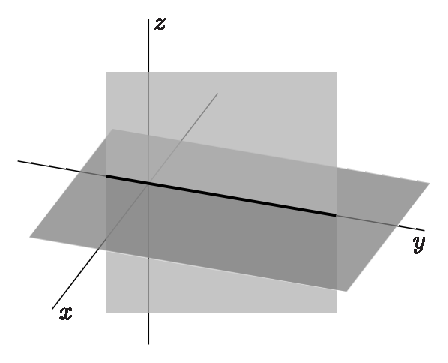
\includegraphics{skript/grafiken/lineare-algebra-2-2-2-a}
\end{center}

\paragraph{Folgerung:}
\begin{itemize}
    \item Der Nullvektor $\vec{0}$ geh�rt zu jeden Unterraum:
    $$ \forall \; U \; \text{ UR } V \text{ gilt } \vec{0} \in U $$
    \item Zu jeden Vektor $\vec{v}$ aus dem Unterraum geh�rt auch der inverse Vektor $- \vec{v}$ zum Unterraum:
    $$ \forall \; U \text{ UR } V \platz \forall \; \vec{v} \in U \text{ gilt } -\vec{v} \in U $$
\end{itemize}

%%%%%%%%%%%%%%%%%%%%%%%%%%%%%%%%%%%%%%%%%%%%%%%%%%%%%%%%%%%%%%%%%%%%%%%%%%%%%%%
\subsection{Linearkombinationen und lineare H�lle}

\paragraph{Definition:} Sind $\veclist{v}{k} \in V$ und $\scalarlist{\lambda}{k} \in K$, so nennt man den Vektor
$$ \veclk{v}{\lambda}{k} $$
eine \emph{Linearkombination}\index{Linearkombination} (LK) aus $\veclist{v}{k}$.

\paragraph{Lemma:} Die Menge aller Linearkombinationen
$$ \{ \veclk{v}{\lambda}{k} \; | \; \lambda_i \in K \} $$
der Vektoren $\veclist{v}{k}$ bildet einen Unterraum. \pagebreak

\paragraph{Beweis:} Seien $\vec{v}, \vec{w} \in U$ und $\alpha \in K$ mit
\begin{itemize}
    \item $\vec{v} = \veclk{u}{\lambda}{k}$
    \item $\vec{w} = \veclk{u}{\mu}{k}$
\end{itemize}
dann gilt:
\begin{eqnarray*}
    \vec{v} + \vec{w} &=& (\veclk{u}{\lambda}{k}) + (\veclk{u}{\mu}{k}) \\
                      &=& (\lambda_1 + \mu_1) \vec{u_1} + (\lambda_2 + \mu_2) \vec{u_2} + \ldots + (\lambda_k + \mu_k) \vec{u}_k \in U \\ \\
    \alpha \vec{v} &=& \alpha (\veclk{u}{\lambda}{k}) \\
                   &=& (\alpha \lambda_1) \vec{u}_1 + (\alpha \lambda_2) \vec{u}_2 + \ldots + (\alpha \lambda_k) \vec{u}_k \in U
\end{eqnarray*}

\paragraph{Definition:} Sei $M \subseteq V$ eine Menge von Vektoren, dann ist die \emph{lineare H�lle}\index{lineare H�lle} (Lin) von $M$ der kleinste (bez�glich Inklusion) Unterraum von $V$, der $M$ enth�lt, d.h.
$$ \text{Lin}(M) = \bigcap_{U \text{ UR } V \atop M \subseteq U} U $$

\paragraph{Satz:} Die lineare H�lle einer Menge $M \subseteq V$ ist die Menge aller Linearkombinationen der Vektoren $\vec{v}_i \in M$:
$$ \text{Lin}(M) = \{ \lambda_1 \vec{v}_1 + \ldots \lambda_k \vec{v}_k \; | \; \lambda_i \in K, \vec{v}_i \in M \} $$

\paragraph{Beweis:} Zum Einen bildet die Menge aller Linearkombinationen der Vektoren $\vec{v}_i \in M$ (rechte Seite) einen Unterraum (siehe Lemma). Zum Anderen enth�lt jeder Unterraum $U$, der $M$ enth�lt, auch die Menge aller Linearkombinationen der Vektoren $\vec{v}_i \in M$ (Abgeschlossenheit von Unterr�umen bez�glich der Addition und der Multiplikation mit Skalaren). Daraus folgt, dass die Menge aller Linearkombinationen der Vektoren $\vec{v}_i \in M$ der kleinste Unterraum ist, der $M$ enth�lt. \pagebreak

%%%%%%%%%%%%%%%%%%%%%%%%%%%%%%%%%%%%%%%%%%%%%%%%%%%%%%%%%%%%%%%%%%%%%%%%%%%%%%%
% Lineare Unabh�ngigkeit, Basis und Dimension
%%%%%%%%%%%%%%%%%%%%%%%%%%%%%%%%%%%%%%%%%%%%%%%%%%%%%%%%%%%%%%%%%%%%%%%%%%%%%%%
\section{Lineare Unabh�ngigkeit, Basis und \mbox{Dimension}}
%%%%%%%%%%%%%%%%%%%%%%%%%%%%%%%%%%%%%%%%%%%%%%%%%%%%%%%%%%%%%%%%%%%%%%%%%%%%%%%
\subsection{Lineare Unabh�ngigkeit}

\paragraph{Definition:} Eine Menge $\{ \veclist{v}{k} \}$ von $k$ Vektoren hei�t \emph{linear abh�ngig}\index{linear abh�ngig} (l.a.), wenn eine Linearkombination existiert, mit
$$ \veclk{v}{\lambda}{k} = \vec{0} $$
wobei mindestens ein $\lambda_i \neq 0$ ist.

\paragraph{Definition:} Eine Menge $\{ \veclist{v}{k} \}$ von $k$ Vektoren hei�t \emph{linear unabh�ngig}\index{linear unabh�ngig} (l.u.), wenn sie nicht linear abh�ngig ist.

\paragraph{Satz:} Eine Menge $M \subseteq V$ ist linear unabh�ngig, wenn jede endliche Teilmenge von $M$ linear unabh�ngig ist.

\paragraph{Folgerungen:}
\begin{enumerate}
    \item Es kann bei \emph{Aufz�hlungen} von Vektoren zu Mehrfachnennungen kommen (im Gegensatz zu Mengen). In diesem Fall folgt lineare Abh�ngigkeit. \par
    Beispiel: Sei $\vec{v}_1, \vec{v}_2, \ldots$ eine Aufz�hlung und $\vec{v}_5 = \vec{v}_7$, dann ist die Aufz�hlung linear abh�ngig, weil
    $$ \vec{0} = 1 \cdot \vec{v}_5 + (-1) \cdot \vec{v}_7 $$
    \item Aus $\vec{0} \in M$ folgt lineare Abh�ngigkeit, denn
    $$ \vec{0} = \lambda \cdot \vec{0} \platz (\text{auch wenn } \lambda \neq 0) $$
    \item Sei $M$ linear unabh�ngig und $\scalarlist{\lambda}{k} \in K$, dann folgt aus
    $$ \forall \; \veclist{v}{k} \in M \platz\platz (i \neq j \; \rightarrow \; \vec{v}_i \neq \vec{v}_j) \platz\platz \vec{0} = \veclk{v}{\lambda}{k} $$
    dass f�r alle $\lambda_i$ gelten muss
    $$ \lambda_i = 0 \platz\platz (i = 1, 2, \ldots k) $$
    Das hei�t: Es existiert \emph{keine} nichttriviale Linearkombination von $\vec{0}$.
    \item Wenn $M$ linear abh�ngig ist, dann existiert eine nichttriviale Linearkombination von $\vec{0}$.
\end{enumerate} \pagebreak

\paragraph{Beispiel:} Die Vektoren
$$ \vecthree{0}{1}{1}, \vecthree{1}{1}{1} \in \real^3 $$
sind linear unabh�ngig, dann ist der Nullvektor $\vec{0}$ ist eine Linearkombination dieser Vektoren:
$$ \vec{0} = \vecthree{0}{0}{0} = \lambda_1 \vecthree{0}{1}{1} + \lambda_2 \vecthree{1}{1}{1} = \vecthree{\lambda_2}{\lambda_1 + \lambda_2}{\lambda_1 + \lambda_2} $$
\begin{eqnarray*}
    0 &=& \lambda_2 \\
    0 &=& \lambda_1 + \lambda_2 \\
    0 &=& \lambda_1 + \lambda_2
\end{eqnarray*}
Daraus folgt, dass $\lambda_1 = \lambda_2 = 0$.

\paragraph{Satz:} F�r jede Teilmenge $M \subseteq V$ (�ber dem K�rper $K$) sind die folgenden Aussagen �quivalent:
\begin{itemize}
    \item Aussage $\text{A}$: \par
    Die Menge $M$ ist linear unabh�ngig.
    \item Aussage $\text{B}$: \par
    Kein Vektor $\vec{v} \in M$ kann als Linearkombination aus den �brigen Vektoren aus $M$ dargestellt werden.
    \item Aussage $\text{C}$: \par
    Jeder Vektor $\vec{v} \in \text{Lin}(M)$ hat \emph{eindeutige} Darstellung als Linearkombination aus $M$.
\end{itemize}

\paragraph{Beweis:} Der Satz wird nach folgendem Schema gezeigt:
$$ \neg \, \text{A} \platz \underset{\text{1. Schritt}}{\Rightarrow} \platz \neg \, \text{B} \platz \underset{\text{2. Schritt}}{\Rightarrow} \platz \neg \, \text{C} \platz \underset{\text{3. Schritt}}{\Rightarrow} \platz \neg \, \text{A} $$
Die drei Aussagen in ihrer Negation:
\begin{itemize}
    \item Aussage $\neg \, \text{A}$: \par
    Es existiert eine nichttriviale Linearkombination von $\vec{0}$.
    \item Aussage $\neg \, \text{B}$: \par
    Es existiert ein Vektor $\vec{v} \in M$, der eine Linearkombination der �brigen Vektoren ist.
    \item Aussage $\neg \, \text{C}$: \par
    Es existiert ein Vektor $\vec{v} \in \text{Lin}(M)$ mit verschiedenen Linearkombinationen aus $M$.
\end{itemize}

Beweisschritte:
\begin{itemize}
    \item Schritt 1: \par
    Es existiert folgende nichttriviale Linearkombination von $\vec{0}$:
    $$ \vec{0} = \veclk{v}{\lambda}{k} $$
    mit $\veclist{v}{k} \in M$, $\scalarlist{\lambda}{k} \in K$ und $\exists \; \lambda_i \neq 0$. \par
    Ohne Beschr�nkung der Allgemeinheit gelte $\lambda_1 \neq 0$. Damit kann die Gleichung nach $\vec{v}_1$ umgeformt werden:
    $$ \vec{v}_1 = \left( - \frac{\lambda_2}{\lambda_1} \right) \vec{v}_2 + \left( - \frac{\lambda_3}{\lambda_1} \right) \vec{v}_3 + \ldots + \left( - \frac{\lambda_k}{\lambda_1} \right) \vec{v}_k $$
    Damit existiert ein Vektor $\vec{v}_1$, der Linearkombination der �brigen Vektoren ist:
    $$ \vec{v}_1 \in \text{Lin}(M \; \backslash \; \{ \vec{v}_1 \}) $$
    \item Schritt 2: \par
    Es existiert ein Vektor $\vec{v}_1$, der Linearkombination der �brigen Vektoren ist:
    $$ \vec{v}_1 = \lambda_2 \vec{v}_2 + \lambda_3 \vec{v}_3 + \ldots + \lambda_k \vec{v}_k $$
    Damit existieren mindestens zwei verschiedene Linearkombinationen von $\vec{v_1}$:
    \begin{eqnarray*}
        \vec{v}_1 &=& 1 \cdot \vec{v}_1 + 0 \cdot \vec{v}_2 + 0 \cdot \vec{v}_3 + \ldots + 0 \cdot \vec{v}_k \\
                  &=& 0 \cdot \vec{v}_1 + \lambda_2 \cdot \vec{v}_2 + \lambda_3 \cdot \vec{v}_3 + \ldots + \lambda_k \cdot \vec{v}_k
    \end{eqnarray*}
    \item Schritt 3: \par
    Es existiert ein Vektor $\vec{v} \in \text{Lin}(M)$ mit verschiedenen Linearkombinationen aus $M$:
    \begin{eqnarray*}
        \vec{v} &=& \veclk{u}{\lambda}{m} \\
                &=& \veclk{w}{\mu}{n}
    \end{eqnarray*}
    mit
    $$ \{ \veclist{u}{m} \} \cup \{ \veclist{w}{n} \} = \{ \veclist{v}{k} \} \subseteq M $$
    Die beiden Linearkombinationen von $\vec{v}$ ausgedr�ckt als Linearkombinationen der die Vektoren aus $\{ \veclist{v}{k} \}$:
    \begin{eqnarray*}
        \vec{v} &=& \veclk{v}{\lambda'}{k} \\
                &=& \veclk{v}{\mu'}{k}
    \end{eqnarray*}
    mit
    $$ \lambda'_i = \left\{ \begin{array}{ll} \lambda_j & \text{ falls } \vec{v}_i = \vec{u}_j \\ 0 & \text{ sonst} \end{array} \right. \hspace{0.5cm} \text{und} \hspace{0.5cm} \mu'_i = \left\{ \begin{array}{ll} \mu_j & \text{ falls } \vec{v}_i = \vec{w}_j \\ 0 & \text{ sonst} \end{array} \right.  $$
    Da es sich um verschiedene Linearkombinationen handelt, existiert ein $i_0$ mit $\lambda'_{i_0} \neq \mu'_{i_0}$. Daraus folgt:
    \begin{eqnarray*}
        \vec{0} &=& \vec{v} - \vec{v} \\
                &=& (\veclk{v}{\lambda'}{k}) - (\veclk{v}{\mu'}{k}) \\
                &=& (\lambda'_1 - \mu'_1) \vec{v}_1 + \ldots + \underbrace{(\lambda'_{i_0} - \mu'_{i_0})}_{\neq 0} \vec{v}_{i_0} + \ldots + (\lambda'_k - \mu'_k) \vec{v}_k
    \end{eqnarray*}
    Damit existiert eine nichttriviale Linearkombination von $\vec{0}$. \hfill $\Box$
    \item Beispiel zu Schritt 3: \par
    \begin{eqnarray*}
        \vectwo{1}{2} &=& 1 \cdot \vectwo{1}{0} + 2 \cdot \vectwo{0}{1} \\
                      &=& 1 \cdot \vectwo{1}{1} + 1 \cdot \vectwo{0}{1}
    \end{eqnarray*}
    Die Menge aller Vektoren, aus beiden Linearkombinationen:
    $$ \left\{ \vectwo{1}{0}, \vectwo{0}{1}, \vectwo{1}{1} \right\} $$
    Die beiden Linearkombinationen mit Hilfe aller Vektoen aus dieser Menge:
    \begin{eqnarray*}
        \vectwo{1}{2} &=& 1 \cdot \vectwo{1}{0} + 2 \cdot \vectwo{0}{1} + 0 \cdot \vectwo{1}{1} \\
                      &=& 0 \cdot \vectwo{1}{0} + 1 \cdot \vectwo{0}{1} + 1 \cdot \vectwo{1}{1}
    \end{eqnarray*}
    Nichttriviale Linearkombination von $\vec{0}$:
    \begin{eqnarray*}
        \vectwo{0}{0} &=& \vectwo{1}{2} - \vectwo{1}{2} \\
                      &=& \left[ 1 \cdot \vectwo{1}{0} + 2 \cdot \vectwo{0}{1} + 0 \cdot \vectwo{1}{1} \right] - \left[ 0 \cdot \vectwo{1}{0} + 1 \cdot \vectwo{0}{1} + 1 \cdot \vectwo{1}{1} \right] \\
                      &=& (1 - 0) \cdot \vectwo{1}{0} + (2 - 1) \cdot \vectwo{0}{1} + (0 - 1) \cdot \vectwo{1}{1} \\
                      &=& 1 \cdot \vectwo{1}{0} + 1 \cdot \vectwo{0}{1} - 1 \cdot \vectwo{1}{1}
    \end{eqnarray*}
\end{itemize}

%%%%%%%%%%%%%%%%%%%%%%%%%%%%%%%%%%%%%%%%%%%%%%%%%%%%%%%%%%%%%%%%%%%%%%%%%%%%%%%
\subsection{Erzeugendensystem und Basis}

\paragraph{Definition:} Eine Teilmenge $M \subseteq V$ hei�t \emph{Erzeugendensystem}\index{Erzeugendensystem} von $V$, wenn die lineare H�lle von $M$ der Vektorraum $V$ ist:
$$ \text{Lin}(M) = V $$

\paragraph{Definition:} Eine Teilmenge $M \subseteq V$ hei�t \emph{Basis}\index{Basis}, wenn sie Erzeugendensystem von~$V$ und linear unabh�ngig ist.

\paragraph{Folgerung:} Eine Teilmenge $M \subseteq V$ ist genau dann eine Basis von $V$, wenn jeder Vektor $\vec{v} \in V$ eine \emph{eindeutige} Darstellung als Linearkombination aus $M$ hat.

\paragraph{Beispiele:}
\begin{itemize}
    \item kanonische Basis von $\real^n$:
    $$ \vec{e}_1 = \vecfour{1}{0}{\vdots}{0}, \hspace{0.5cm} \vec{e}_2 = \vecfour{0}{1}{\vdots}{0}, \hspace{0.5cm} \ldots \hspace{0.5cm} \vec{e}_n = \vecfour{0}{0}{\vdots}{1} $$
    F�r die kanonische Basis gilt:
    $$ \vecfour{a_1}{a_2}{\vdots}{a_n} = a_1 \vec{e}_1 + a_2 \vec{e}_2 + \ldots + a_n \vec{e}_n $$
    \item weitere Basis von $\real^n$:
    $$ \vec{e}_1 = \vecfour{1}{0}{\vdots}{0}, \hspace{0.5cm} \vec{e}_2 = \vecfour{1}{1}{\vdots}{0}, \hspace{0.5cm} \ldots \hspace{0.5cm} \vec{e}_n = \vecfour{1}{1}{\vdots}{1} $$
    \item Standardbasis f�r den Vektorraum $\real[x]$ der Polynome:
    $$ \vec{e}_1 = 1, \hspace{0.5cm} \vec{e}_2 = x, \hspace{0.5cm} \vec{e}_3 = x^2, \hspace{0.5cm} \ldots $$
\end{itemize}

\paragraph{Folgerung:} F�r jede Teilmenge $M \subseteq V$ sind die folgenden Bedingungen �quivalent:
\begin{itemize}
    \item Aussage $\text{A}$: \par
    Die Menge $M$ ist Basis von $V$.
    \item Aussage $\text{B}$: \par
    Die Menge $M$ ist minimales Erzeugendensystem von $V$.
    \item Aussage $\text{C}$: \par
    Die Menge $M$ ist eine maximale linear unabh�ngige Menge.
\end{itemize}
Bemerkung: Die Begriffe "`minimal"' und "`maximal"' gelten in Bezug auf Inklusion.

\paragraph{Lemma:} Ist die Teilmenge $M \subseteq V$ linear unabh�ngig und der Vektor $\vec{v}$ Element von $V$, aber nicht Element aus der linearen H�llen von $M$, dann ist die Menge $M \cup \{ \vec{v} \}$ ebenfalls linear unabh�ngig:
$$ M \subseteq V \text{ l.u.} \platz \land \platz \vec{v} \in V \platz \land \platz \vec{v} \notin \text{Lin}(M) \platz \Rightarrow \platz M \cup \{ \vec{v} \} \text{ l.u.} $$

\paragraph{Beweis (indirekt):} Angenommen die Teilmenge $M \subseteq V$ ist linear unabh�ngig und der Vektor $\vec{v}$ Element von $V$, aber nicht Element aus der linearen H�llen von $M$, und die Menge $M \cup \{ \vec{v} \}$ ist linear abh�ngig. Damit existiert eine nichttriviale Linearkombination von $\vec{0}$ (mit $\exists \, \lambda_i \neq 0 \; \lor \; \lambda \neq 0$):
$$ \vec{0} = \veclk{v}{\lambda}{k} + \lambda \vec{v} $$
Wenn $\lambda \neq 0$, dann l�sst sich die Gleichung nach $\vec{v}$ umformen:
$$ \vec{v} = \left( - \frac{\lambda_1}{\lambda} \right) \vec{v}_1 + \left( - \frac{\lambda_2}{\lambda} \right) \vec{v}_2 + \ldots + \left( - \frac{\lambda_k}{\lambda} \right) \vec{v}_k $$
Damit ist der Vektor $\vec{v}$ in der linearen H�llen von $M$:
$$ \vec{v} \in \text{Lin}(M) $$
Dies w�re ein Widerspruch zur Annahme. Damit ist $\lambda = 0$. Daraus folgt:
$$ \exists \, \lambda_i \neq 0 \hspace{0.5cm} \vec{0} = \veclk{v}{\lambda}{k} $$
Dies ist ein Widerspruch, da die Menge $M$ linear unabh�ngig ist und damit keine nichttriviale Linearkombination von $\vec{0}$ existiert. \hfill $\Box$

\paragraph{Basiserg�nzungssatz (Steinitz)\index{Basiserg�nzungssatz}\index{Steinitz (Basiserg�nzungssatz)}:} Seien
\begin{itemize}
    \item $V$ ein Vektorraum �ber dem K�rper $K$
    \item $M$ eine Teilmenge von $V$
    \item $N$ eine Teilmenge von $V$
\end{itemize}
Ist die Menge $M$ linear unabh�ngig und die lineare H�lle von $M \cup N$ der Vektorraum~$V$, dann kann man die Menge $M$ durch eventuelle Hinzunahme von Vektoren aus der Menge $N$ zu einer Basis des Vektorraumes $V$ erweitern.

\paragraph{Beweis:} Induktion nach $k = |N|$:
\begin{itemize}
    \item Induktionsanfang ($k = 0$, das hei�t $N = \emptyset$): \par
    Die Menge $M$ ist Basis, weil $M$ linear unabh�ngig ist und
    $$ \text{Lin}(M) = \text{Lin}(M \cup \emptyset) = \text{Lin}(M \cup N) = V $$
    \item Induktionsschritt ($k - 1 \rightarrow k$): \par
    \begin{itemize} \punkt
        \item Fall 1: $\text{Lin}(M) = V$ \par
        Daraus folgt, dass die Menge $M$ Basis ist.
        \item Fall 2: $\text{Lin}(M) \neq V$ \par
        Sei der Vektor $\vec{v}$ Element von $N$, aber nicht Element aus der linearen H�llen von $M$. Damit ist die Menge $M \cup \{ \vec{v} \}$ ebenfalls linear unabh�ngig. \par
        Die Menge $M$ wird also um den Vektor $\vec{v}$ erweitert, und die Menge $N$ wird um den Vektor $\vec{v}$ reduziert:
        $$ | N \; \backslash \; \{ \vec{v} \} | = k - 1 $$
        Nach Induktionsvoraussetzung existiert eine Erweiterung der Menge~$M$ zur Basis.
    \end{itemize}
\end{itemize} \hfill $\Box$ \pagebreak

\paragraph{Beispiele:}
\begin{enumerate}
    \item Sei $M_1$ die folgende linear unabh�ngige Menge und $N_1$ die kanonische Basis von $\real^3$:
    $$ M_1 = \left\{ \vecthree{1}{1}{0}, \vecthree{0}{1}{1} \right\} $$
    Man kann jeden der drei Vektoren aus $N_1$ als Basiserg�nzung w�hlen.
    \item Sei $M_2$ die folgende linear unabh�ngige Menge und $N_2$ die kanonische Basis von $\real^3$:
    $$ M_2 = \left\{ \vecthree{1}{0}{0}, \vecthree{1}{1}{0} \right\} $$
    Der Vektor $\vec{e}_1$ ist bereits in $M_2$ enthalten und damit keine Erg�nzung von~$M_2$, der Vektor $\vec{e}_2$ ist auch keine Basiserg�nzung, weil $M_2 \cup \{ \vec{e}_2 \}$ linear abh�ngig w�re, doch der dritte Vektor $\vec{e}_3$ erg�nzt die Menge $M_2$ zu einer Basis.
\end{enumerate}

\paragraph{Austauschlemma:} Sind die Mengen $\{ \veclist{v}{n} \}$ und $\{ \veclist{w}{m} \}$ Basen von $V$, dann gibt es f�r jeden Vektor $\vec{v}_i$ einen Vektor $\vec{w}_j$, so dass die Menge
$$ \left( \{ \veclist{v}{n} \} \; \backslash \; \{ \vec{v}_i \} \right) \cup \{ \vec{w}_j \} $$
ebenfalls Basis von $V$ ist.

%%%%%%%%%%%%%%%%%%%%%%%%%%%%%%%%%%%%%%%%%%%%%%%%%%%%%%%%%%%%%%%%%%%%%%%%%%%%%%%
\subsection{Dimension}

\paragraph{Definition:} Besitzt ein Vektorraum $V$ eine endliche Basis $\{ \veclist{v}{n} \}$, dann ist $V$ \emph{endlich-dimensional}\index{endlich-dimensional} und $n$ hei�t die \emph{Dimension}\index{Dimension} von $V$:
$$ \text{dim } V = n $$
Ein Vektorraum, der keine endliche Basis besitzt, ist \emph{unendlich-dimensional}\index{unendlich-dimensional}:
$$ \text{dim } V = \infty $$

\paragraph{Folgerung:} Ist die Menge $M = \{ \veclist{v}{k} \}$ Teilmenge eines Vektorraums $V$ und ist $k > \text{dim } V$, so ist $M$ linear abh�ngig.

\paragraph{Satz:} Jeder Vektorraum besitzt eine Basis.

\paragraph{Satz:} Ist die Dimension eines Vektorraumes $V$ endlich und $U$ ein Unterraum von $V$, dann gilt:
$$ \text{dim } U \leq \text{dim } V $$
und
$$ \text{dim } U < \text{dim } V \platz \Leftrightarrow \platz U \neq V $$

\paragraph{Definition:} Sind $U_1$ und $U_2$ Unterr�ume von $V$, so hei�t
$$ U_1 + U_2 = \{ \vec{x} + \vec{y} \; | \; \vec{x} \in U_1, \vec{y} \in U_2 \} $$
die Summe von $U_1$ und $U_2$\index{Summe von Unterr�umen}.

\paragraph{Beispiele:}
\begin{enumerate}
    \item Sei $V = \real^4$:
    \begin{eqnarray*}
        U_1 &=& \text{Lin}(\{ \vec{e}_1, \vec{e}_2, \vec{e}_4 \}) \\
        U_2 &=& \text{Lin}(\{ \vec{e}_1, \vec{e}_3, \vec{e}_4 \}) \\ \\
        U_1 + U_2 &=& \real^4
    \end{eqnarray*}
    \item Sei $V = \real^3$:
    \begin{eqnarray*}
        U_1 &=& \text{Lin} \left( \left\{ \vecthree{1}{-1}{1} \right\} \right) \\
        U_2 &=& \text{Lin} \left( \left\{ \vecthree{1}{-1}{-1} \right\} \right) \\ \\
        U_1 + U_2 &=& \text{Lin} \left( \left\{ \vecthree{1}{-1}{1}, \vecthree{1}{-1}{-1} \right\} \right) = \text{Lin} \left( \left\{ \vecthree{1}{-1}{0}, \vecthree{0}{0}{1} \right\} \right)
    \end{eqnarray*}
    Bemerkung: $U_1 + U_2$ ist die Ebene senkrecht zu $xy$-Ebene auf der Geraden~$y = -x$ durch den Ursprung $(0, 0, 0)$.
\end{enumerate}

\paragraph{Satz:} Die Summe von zwei Unterr�umen ist ein Unterraum. F�r zwei endlich-dimensionale Unterr�ume $U_1$ und $U_2$ gilt:
$$ \text{dim}(U_1 + U_2) = \text{dim } U_1 + \text{dim } U_2 - \text{dim}(U_1 \cap U_2) $$

\paragraph{Beweisidee:}
\begin{itemize}
    \item Die Basis von $U_1 \cap U_2$ sei:
    $$ \{ \veclist{v}{r} \} $$
    \item Erg�nzung der Basis von $U_1 \cap U_2$ zur Basis von $U_1$:
    $$ \{ \veclist{v}{r}, \veclist{u}{s} \} $$
    \item Erg�nzung der Basis von $U_1 \cap U_2$ zur Basis von $U_2$:
    $$ \{ \veclist{v}{r}, \veclist{w}{t} \} $$
    \item Man zeigt: Die Basis von $U_1 + U_2$ ist:
    $$ \{ \veclist{v}{r}, \veclist{u}{s}, \veclist{w}{t} \} $$
    \item Damit gilt f�r die Dimenstionen:
    \begin{itemize}
        \item $\text{dim}(U_1 + U_2) = r + s + t$
        \item $\text{dim } U_1 = r + s$
        \item $\text{dim } U_2 = r + t$
        \item $\text{dim}(U_1 \cap U_2) = r$
    \end{itemize}
    Daraus folgt:
    $$ \underbrace{\text{dim}(U_1 + U_2)}_{r + s + t} = \underbrace{\text{dim } U_1}_{r + s} + \underbrace{\text{dim } U_2}_{r + t} - \underbrace{\text{dim}(U_1 \cap U_2)}_{r} $$
\end{itemize}

\paragraph{Beispiele:}
\begin{enumerate}
    \item Sei $U_1$ eine Ebene durch den Ursprung $(0, 0, 0)$ und $U_2$ eine Gerade durch den Ursprung $(0, 0, 0)$ mit $U_2 \not\subset U_1$. Daraus hei�t:
    \begin{itemize}
        \item $\text{dim } U_1 = 2$
        \item $\text{dim } U_2 = 1$
        \item $\text{dim}(U_1 \cap U_2) = 0$ (weil $U_1 \cap U_2 = \vec{0}$)
    \end{itemize}
    Daraus folgt:
    \begin{itemize}
        \item $\text{dim}(U_1 + U_2) = 3$
    \end{itemize}
    Damit ist $U_1 + U_2 = \real^3$.
    \item Seien $U_1$ und $U_2$ Ebenen durch den Ursprung $(0, 0, 0)$ mit $U_1 \neq U_2$. Daraus hei�t:
    \begin{itemize}
        \item $\text{dim } U_1 = 2$
        \item $\text{dim } U_2 = 2$
        \item $\text{dim}(U_1 \cap U_2) = 1$ (weil $U_1 \cap U_2$ eine Gerade ist)
    \end{itemize}
    Daraus folgt:
    \begin{itemize}
        \item $\text{dim}(U_1 + U_2) = 3$
    \end{itemize}
    Damit ist $U_1 + U_2 = \real^3$.
\end{enumerate}

%%%%%%%%%%%%%%%%%%%%%%%%%%%%%%%%%%%%%%%%%%%%%%%%%%%%%%%%%%%%%%%%%%%%%%%%%%%%%%%
% Lineare Abbildungen
%%%%%%%%%%%%%%%%%%%%%%%%%%%%%%%%%%%%%%%%%%%%%%%%%%%%%%%%%%%%%%%%%%%%%%%%%%%%%%%
\section{Lineare Abbildungen}
%%%%%%%%%%%%%%%%%%%%%%%%%%%%%%%%%%%%%%%%%%%%%%%%%%%%%%%%%%%%%%%%%%%%%%%%%%%%%%%
\subsection{Einleitung}

\paragraph{Definition:} Seien $V$ und $W$ Vektorr�ume �ber dem K�rper $K$. Eine Abbildung $f : V \rightarrow W$ hei�t \emph{linear}\index{lineare Abbildung} \emph{(Vektorraumhomomorphismus)}\index{Vektorraumhomomorphismus}\index{Homomorphismus}, wenn f�r alle $\vec{v}, \vec{w} \in V$ und f�r alle $\lambda \in K$ gilt:
\begin{eqnarray*}
    f(\vec{v} + \vec{w}) &=& f(\vec{v}) + f(\vec{w}) \\
    f(\lambda \cdot \vec{v}) &=& \lambda \cdot f(\vec{v})
\end{eqnarray*}
$\text{Hom}(V, W)$ bezeichnet die Menge aller linearer Abbildungen $f : V \rightarrow W$.

\paragraph{Beobachtungen:}
\begin{itemize}
    \item Sei $f \in \text{Hom}(V, W)$, dann gilt:
    $$ f(\veclk{v}{\lambda}{k}) = \lambda_1 \cdot f(\vec{v}_1) + \lambda_2 \cdot f(\vec{v}_2) + \ldots + \lambda_k \cdot f(\vec{v}_k) $$
    \item Die Verkn�pfung von linearen Abbildungen $f : V \rightarrow W$ und $g : W \rightarrow Y$ ist eine lineare Abbildung $gf : V \rightarrow Y$ mit
    $$ gf(\vec{v}) = g(f(\vec{v})) $$
    \item Die Menge aller linearen Abbildungen $\text{Hom}(V, W)$ ist selbst ein Vektorraum mit den Operationen:
    \begin{itemize} \punkt
        \item $(f + g)(\vec{v}) = f(\vec{v}) + g(\vec{v})$
        \item $(\lambda \cdot f)(\vec{v}) = \lambda \cdot f(\vec{v})$
    \end{itemize}
    Denn f�r alle $f, g \in \text{Hom}(V, W)$, $\vec{u}, \vec{v} \in V$ und $\lambda \in K$:
    \begin{eqnarray*}
        (f+g)(\vec{u}) + (f+g)(\vec{v}) &=& f(\vec{u}) + g(\vec{u}) + f(\vec{v}) + g(\vec{v}) \\
                                        &=& f(\vec{u}) + f(\vec{u}) + g(\vec{v}) + g(\vec{v}) \\
                                        &=& f(\vec{u}+\vec{v}) + g(\vec{u} + \vec{v}) \\
                                        &=& (f+g)(\vec{u}+\vec{v}) \\ \\
                                        &\rightarrow& f+g \in \text{Hom}(V, W) \\ \\
        \lambda \cdot (f+g)(\vec{u}) &=& \lambda \cdot (f(\vec{u}) + g(\vec{u})) \\
                                     &=& \lambda \cdot f(\vec{u}) + \lambda \cdot g(\vec{u}) \\
                                     &=& f(\lambda \vec{u}) + g(\lambda \vec{u}) \\
                                     &=& (f+g)(\lambda \vec{u}) \\ \\
                                     &\rightarrow& \lambda \cdot f \in \text{Hom}(V, W)
    \end{eqnarray*}
\end{itemize}

\paragraph{Beispiele:} $f, g, h, j : \real^2 \rightarrow \real^2$ \label{linabb}
\begin{enumerate} \buchstaben
    \item Spiegelung an der $x$-Achse :
    $$ f \left( \vectwo{x}{y} \right) = \vectwo{x}{-y} $$
    \begin{center}
        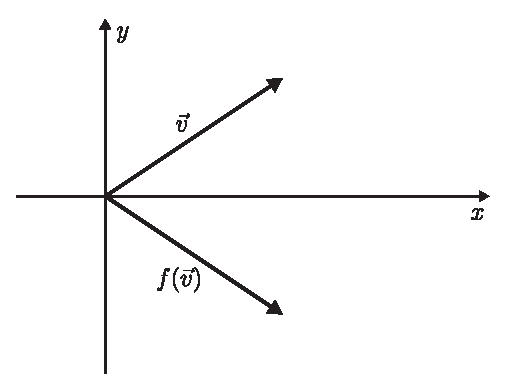
\includegraphics{skript/grafiken/lineare-algebra-2-4-1-a}
    \end{center} \pagebreak
    \item Spiegelung an der Geraden $y = x$:
    $$ g \left( \vectwo{x}{y} \right) = \vectwo{y}{x} $$
    \begin{center}
        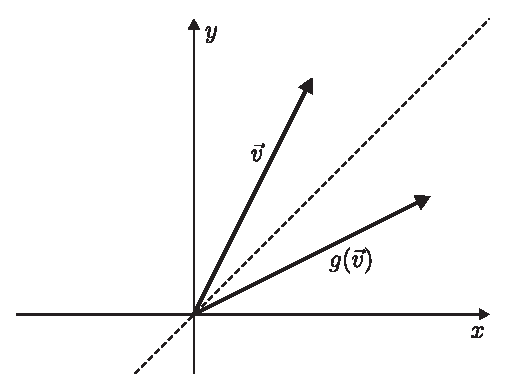
\includegraphics{skript/grafiken/lineare-algebra-2-4-1-b}
    \end{center}
    \item Projektion auf die $y$-Achse:
    $$ h \left( \vectwo{x}{y} \right) = \vectwo{0}{y} $$
    \begin{center}
        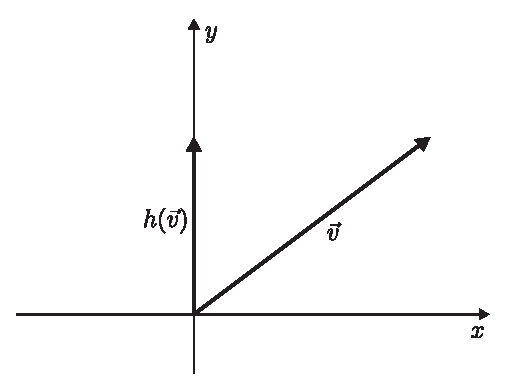
\includegraphics{skript/grafiken/lineare-algebra-2-4-1-c}
    \end{center}
    \item Drehung um 45�:
    \begin{eqnarray*}
        j \left( \vectwo{1}{0} \right) &=& \vectwo{\frac{1}{\sqrt{2}}}{\frac{1}{\sqrt{2}}} \\
        j \left( \vectwo{0}{1} \right) &=& \vectwo{-\frac{1}{\sqrt{2}}}{\frac{1}{\sqrt{2}}} \\ \\ \\
        j \left( \vectwo{x}{y} \right) &=& j \left( x \vectwo{1}{0} + y \vectwo{0}{1} \right) \\ \\
                                       &=& x \cdot j \left( \vectwo{1}{0} \right) + y \cdot j \left( \vectwo{0}{1} \right) \\ \\
                                       &=& x \cdot \vectwo{\frac{1}{\sqrt{2}}}{\frac{1}{\sqrt{2}}} + y \cdot \vectwo{-\frac{1}{\sqrt{2}}}{\frac{1}{\sqrt{2}}} \\ \\
                                       &=& \vectwo{\frac{1}{\sqrt{2}} \; x - \frac{1}{\sqrt{2}} \; y}{\frac{1}{\sqrt{2}} \; x + \frac{1}{\sqrt{2}} \; y}
    \end{eqnarray*}
    \begin{center}
        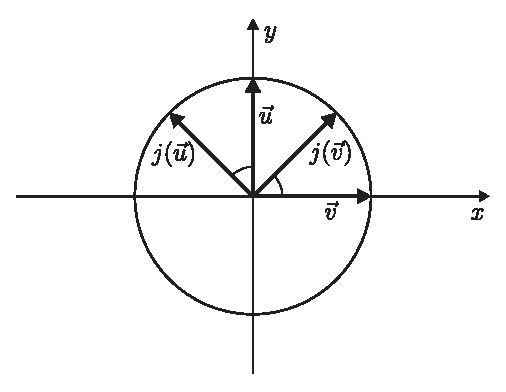
\includegraphics{skript/grafiken/lineare-algebra-2-4-1-d}
    \end{center}
\end{enumerate} \pagebreak

%%%%%%%%%%%%%%%%%%%%%%%%%%%%%%%%%%%%%%%%%%%%%%%%%%%%%%%%%%%%%%%%%%%%%%%%%%%%%%%
\subsection{Kern und Bild von linearen Abbildungen}

\paragraph{Definition:} Sei $f \in \text{Hom}(V,W)$ eine lineare Abbildung, so ist ihr \emph{Kern}\index{Kern einer linearen Abbildung} ($\text{Ker } f$) und ihr \emph{Bild}\index{Bild einer linearen Abbildung} ($\text{Im } f$) folgenderma�en definiert:
\begin{eqnarray*}
    \text{Ker } f &=& \{ \vec{v} \in V \; | \; f(\vec{v}) = \vec{0} \} \\
    \text{Im } f &=& \{ \vec{w} \in W \; | \; \exists \, \vec{v} \; \; f(\vec{v}) = \vec{w} \}
\end{eqnarray*}

\paragraph{Beispiele:} Kerne und Bilder aus dem obigen Beispiel (siehe \ref{linabb})
\begin{enumerate} \buchstaben
    \item $\text{Ker } f = \{ \vec{0} \}$:
    $$ f \left( \vectwo{x}{y} \right) = \vectwo{x}{-y} = \vectwo{0}{0} \platz \Leftrightarrow \platz x = 0 \platz \land \platz y = 0 $$
    $\text{Im } f = \real^2$:
    \begin{itemize}
        \item $f$ ist eine Abbildung von $\real^2$ nach $\real^2$, und zwar $f^{-1} = f$.
    \end{itemize}

    \item $\text{Ker } g = \{ \vec{0} \}$:
    $$ g \left( \vectwo{x}{y} \right) = \vectwo{y}{x} = \vectwo{0}{0} \platz \Leftrightarrow \platz x = 0 \platz \land \platz y = 0 $$
    $\text{Im } g = \real^2$:
    \begin{itemize}
        \item $g$ ist eine Abbildung von $\real^2$ nach $\real^2$, und zwar $g^{-1} = g$.
    \end{itemize}

    \item $\text{Ker } h = \text{Lin} \left( \vectwo{1}{0} \right)$:
    $$ h \left( \vectwo{x}{y} \right) = \vectwo{0}{y} = \vectwo{0}{0} \platz \Leftrightarrow \platz y = 0 $$
    $\text{Im } h = \text{Lin} \left( \vectwo{0}{1} \right)$:
    \begin{itemize}
        \item die $x$-Komponente aller Elemente aus dem Bild ist $0$.
    \end{itemize}

    \item $\text{Ker } j = \{ \vec{0} \}$:
    $$ j \left( \vectwo{x}{y} \right) = \vectwo{\frac{1}{\sqrt{2}} \; x - \frac{1}{\sqrt{2}} \; y}{\frac{1}{\sqrt{2}} \; x + \frac{1}{\sqrt{2}} \; y} = \vectwo{0}{0} \platz \Leftrightarrow \platz x = 0 \platz \land \platz y = 0 $$
    $\text{Im } f = \real^2$:
    \begin{itemize}
        \item $j$ ist eine Abbildung von $\real^2$ nach $\real^2$ und $j$ ist bijektiv, so dass folgende Umkehrabbildung existiert:
        $$ j^{-1} \left( \vectwo{x}{y} \right) = \vectwo{\frac{1}{\sqrt{2}} \; x + \frac{1}{\sqrt{2}} \; y}{- \frac{1}{\sqrt{2}} \; x + \frac{1}{\sqrt{2}} \; y} $$
    \end{itemize}
\end{enumerate}

\paragraph{Lemma:} Der Kern und das Bild einer linearen Abbildung $f \in \text{Hom}(V, W)$ sind Unterr�ume von $V$ bzw. $W$:
\begin{eqnarray*}
    \text{Ker } f &\text{UR}& V \\
    \text{Im } f &\text{UR}& W
\end{eqnarray*}

\paragraph{Beweis (Kern):} Seien $\vec{u}, \vec{v} \in \text{Ker } f$ und $\lambda \in K$ (K�rper zu $V$).
\begin{itemize}
    \item Pr�fe, ob $\text{Ker } f$ mindestens ein Element enth�lt:
    \begin{eqnarray*}
        f(\vec{0}) &=& f(\vec{0} - \vec{0}) \\
                   &=& f(\vec{0}) - f(\vec{0}) \\
                   &=& \vec{0}
    \end{eqnarray*}
    Damit ist $\vec{0} \in \text{Ker } f$.
    \item Pr�fe Abgeschlossenheit gegen�ber der Addition:
    \begin{eqnarray*}
        f(\vec{u} + \vec{v}) &=& f(\vec{u}) + f(\vec{v}) \\
                             &=& \vec{0} + \vec{0} \hspace{0.5cm} \text{(da $\vec{u}, \vec{v} \in \text{Ker } f$)} \\
                             &=& \vec{0}
    \end{eqnarray*}
    Damit ist auch $\vec{u} + \vec{v} \in \text{Ker } f$.
    \item Pr�fe Abgeschlossenheit gegen�ber der Multiplikation mit Skalaren:
    \begin{eqnarray*}
        f(\lambda \vec{u}) &=& \lambda \cdot f(\vec{u}) \\
                           &=& \lambda \cdot \vec{0} \hspace{0.5cm} \text{(da $\vec{u} \in \text{Ker } f$)} \\
                           &=& \vec{0}
    \end{eqnarray*}
    Damit ist auch $\lambda \vec{u} \in \text{Ker } f$. \hfill $\Box$
\end{itemize}

\paragraph{Beweis (Bild):} Seien $\vec{u}, \vec{v} \in \text{Im } f$ und $\lambda \in K$ (K�rper zu $W$).
\begin{itemize}
    \item Pr�fe, ob $\text{Im } f$ mindestens ein Element enth�lt:
    \begin{eqnarray*}
        f(\vec{0}) &=& \vec{0} \hspace{0.5cm} \text{(siehe oben)}
    \end{eqnarray*}
    Damit ist $\vec{0} \in \text{Im } f$.
    \item Pr�fe Abgeschlossenheit gegen�ber der Addition:
    \begin{eqnarray*}
        \vec{u} + \vec{v} &=& f(\vec{p}) + f(\vec{q}) \hspace{0.5cm} \text{(mit $f(\vec{p}) = \vec{u}$ und $f(\vec{q}) = \vec{v}$)} \\
                          &=& f(\vec{p} + \vec{q}) \\
                          &=& f(\vec{r}) \hspace{0.5cm} \text{(mit $\vec{r} = \vec{p} + \vec{q} \in V$)}
    \end{eqnarray*}
    Damit ist auch $\vec{u} + \vec{v} \in \text{Im } f$.
    \item Pr�fe Abgeschlossenheit gegen�ber der Multiplikation mit Skalaren:
    \begin{eqnarray*}
        \lambda \vec{u} &=& \lambda \cdot f(\vec{p}) \hspace{0.5cm} \text{(mit $f(\vec{p}) = \vec{u}$)} \\
                        &=& f(\lambda \vec{p}) \\
                        &=& f(\vec{r}) \hspace{0.5cm} \text{(mit $\vec{r} = \lambda \vec{p} \in V$)}
    \end{eqnarray*}
    Damit ist auch $\lambda \vec{u} \in \text{Im } f$. \hfill $\Box$
\end{itemize}

\paragraph{Lemma:} Eine lineare Abbildung $f \in \text{Hom}(V, W)$ ist genau dann injektiv, wenn ihr Kern nur aus dem Nullvektor besteht:
$$ \text{Ker } f = \{ \vec{0} \} $$

\paragraph{Beweis ($\Rightarrow$):} Da $f(\vec{0}) = \vec{0}$ und $f$ injektiv ist, bildet kein anderer Vektor auf $\vec{0}$ ab. Damit liegt au�er dem Nullvektor kein anderer Vektor im $\text{Ker } f$. \hfill $\Box$
\paragraph{Beweis durch Widerspruch ($\Leftarrow$):} Angenommen $\text{Ker } f = \{ \vec{0} \}$ und $f$ ist \emph{nicht} injektiv, dann existieren zwei Vektoren $\vec{u}, \vec{v} \in V$, so dass
$$ \vec{u} \neq \vec{v} \platz \land \platz f(\vec{u}) = f(\vec{v}) $$
Daraus folgt:
$$ f(\vec{u} - \vec{v}) = f(\vec{u}) - f(\vec{w}) = \vec{0} $$
Damit liegt $\vec{u} - \vec{v} \neq \vec{0}$ in $\text{Ker } f$. Dies ist ein Widerspruch, da $\text{Ker } f = \{ \vec{0} \}$. \hfill $\Box$

%%%%%%%%%%%%%%%%%%%%%%%%%%%%%%%%%%%%%%%%%%%%%%%%%%%%%%%%%%%%%%%%%%%%%%%%%%%%%%%
\subsection{Spezielle Homomorphismen}

\paragraph{Definitionen:} Einen Homomorphismus $f \in \text{Hom}(V, W)$ nennt man einen
\begin{itemize}
    \item \emph{Monomorphismus}\index{Monomorphismus}, wenn $f$ injektiv ist,
    \item \emph{Epimorphismus}\index{Epimorphismus}, wenn $f$ surjektiv ist,
    \item \textbf{\emph{Isomorphismus}}\index{Isomorphismus}, wenn $f$ bijektiv ist,
    \item \emph{Endomorphismus}\index{Endomorphismus}, wenn $V = W$,
    \item \textbf{\emph{Automorphismus}}\index{Automorphismus}, wenn $V = W$ und $f$ bijektiv ist.
\end{itemize}

\paragraph{Satz:} Ist $f \in \text{Hom}(V, W)$ ein Isomorphismus, dann ist auch $f^{-1} \in \text{Hom}(W, V)$ ein Isomorphismus.

\paragraph{Satz:} Die Verkettung von Isomorphismen ist auch wieder ein Isomorphismus.

\paragraph{Satz:} Seien
\begin{itemize}
    \item $V, W$ Vektorr�ume �ber $K$,
    \item die Menge $\{ \veclist{v}{n} \} \subseteq V$ eine Basis von $V$ und
    \item $\veclist{w}{n} \in W$ beliebig,
\end{itemize}
dann gibt es eine \emph{eindeutige} lineare Abbildung $f \in \text{Hom}(V, W)$ definiert durch
$$ f(\vec{v}_i) = \vec{w}_i \platz \text{f�r} \platz i = 1, 2, \ldots n $$

\paragraph{Beweis:} Jeder Vektor $\vec{v} \in V$ hat eine eindeutige Darstellung als Linearkombination aus $\{ \veclist{v}{n} \}$:
$$ \vec{v} = \veclk{v}{\lambda}{n} $$
\begin{itemize}
    \item Zu zeigen ist, dass eine entsprechende lineare Abbildung existiert. Dazu wird die Abbildung des Vektors $\vec{v}$ folgenderma�en definiert:
    \begin{eqnarray*}
        f(\vec{v}) &=& \veclk{w}{\lambda}{n} \\
                   &=& \lambda_1 \cdot f(\vec{v}_1) + \lambda_2 \cdot f(\vec{v}_2) + \ldots + \lambda_n \cdot f(\vec{v}_n)
    \end{eqnarray*}
    Au�erdem gilt:
    $$ f(\vec{v}) = f(\veclk{v}{\lambda}{n}) $$
    Daraus folgt:
    $$ f(\veclk{v}{\lambda}{n}) = \lambda_1 \cdot f(\vec{v}_1) + \lambda_2 \cdot f(\vec{v}_2) + \ldots + \lambda_n \cdot f(\vec{v}_n) $$
    Damit ist $f$ eine lineare Abbildung.
    \item Au�erdem ist zu zeigen, dass $f$ eine eindeutige lineare Abbildung ist: \par
    Angenommen es existiert eine lineare Abbildung $g \neq f$ mit $g(\vec{v}_i) = \vec{w}_i$. Damit gilt:
    \begin{eqnarray*}
        g(\vec{v}) &=& g(\veclk{v}{\lambda}{n}) \\
                   &=& \lambda_1 \cdot g(\vec{v}_1) + \lambda_2 \cdot g(\vec{v}_2) + \ldots + \lambda_n \cdot g(\vec{v}_n) \\
                   &=& \veclk{w}{\lambda}{n} \\
                   &=& f(\vec{v})
    \end{eqnarray*}
    Das hei�t, f�r alle $\vec{v} \in V$ gilt $g(\vec{v}) = f(\vec{v})$. Damit ist $g = f$. Dies ein Widerspruch zur Annahme. \hfill $\Box$
\end{itemize}

\paragraph{Folgerung:} Zu zwei $n$-dimentionalen Vektorr�umen existiert mindestens ein Isomorphismus, der den einen Vektorraum in den anderen �berf�hrt.

%%%%%%%%%%%%%%%%%%%%%%%%%%%%%%%%%%%%%%%%%%%%%%%%%%%%%%%%%%%%%%%%%%%%%%%%%%%%%%%
\subsection{Rang einer linearen Abbildung}

\paragraph{Definition:} Der \emph{Rang}\index{Rang einer linearen Abbildung} einer linearen Abbildung $f \in \text{Hom}(V, W)$ ist die Dimension des Bildes von $f$:
$$ \text{rg } f = \text{dim}(\text{Im f}) $$

\paragraph{Satz (Dimensionsformel f�r lineare Abbildungen\index{Dimensionsformel}):} F�r jede lineare Abbildung $f \in \text{Hom}(V, W)$ gilt:
$$ \begin{array}{ccccc}
    \text{dim}(\text{Ker } f) &+& \text{dim}(\text{Im } f) &=& \text{dim } V \\
    \text{dim}(\text{Ker } f) &+& \text{rg } f &=& \text{dim } V
\end{array} $$

\paragraph{Beweis:} Sei $\{ \veclist{v}{k} \}$ eine Basis von $\text{Ker } f \subseteq V$:
$$ \text{Ker } f = \text{Lin}(\{ \veclist{v}{k} \}) \platz \text{und} \platz \{ \veclist{v}{k} \} \text{ ist l.u.} $$
Diese Basis wird durch die Vektoren $\{ \vec{v}_{k+1}, \vec{v}_{k+2}, \ldots \vec{v}_n \}$ zu einer Basis von $V$ erweitert:
$$ V = \text{Lin}(\{ \vec{v}_1, \ldots \vec{v}_k, \vec{v}_{k+1}, \ldots \vec{v}_n \}) \platz \text{und} \platz \{ \vec{v}_1, \ldots \vec{v}_k, \vec{v}_{k+1}, \ldots \vec{v}_n \} \text{ ist l.u.} $$
Zu zeigen ist, dass $\{ f(\vec{v}_{k+1}), f(\vec{v}_{k+2}), \ldots f(\vec{v}_n) \}$ eine Basis von $\text{Im } f$ ist.
\begin{itemize}
    \item Angenommen $\vec{w} \in \text{Im } f$:
    \begin{eqnarray*}
        \vec{w} &=& f(\vec{v}) \\
                &=& f(\lambda_1 \cdot \vec{v}_1 + \ldots + \lambda_k \cdot \vec{v}_k + \lambda_{k+1} \cdot \vec{v}_{k+1} + \ldots + \lambda_n \cdot \vec{v}_n) \\
                &=& \lambda_1 \cdot f(\vec{v}_1) + \ldots + \lambda_k \cdot f(\vec{v}_k) + \lambda_{k+1} \cdot f(\vec{v}_{k+1}) + \ldots + \lambda_n \cdot f(\vec{v}_n)
    \end{eqnarray*}
    Da $\veclist{v}{k} \in \text{Ker } f$, gilt $f(\vec{v}_1) = f(\vec{v}_2) = \ldots = f(\vec{v}_k) = \vec{0}$. Daraus folgt:
    $$ \vec{w} = \lambda_{k+1} \cdot f(\vec{v}_{k+1}) + \lambda_{k+2} \cdot f(\vec{v}_{k+2}) + \ldots + \lambda_n \cdot f(\vec{v}_n) $$
    Damit ist $\{ f(\vec{v}_{k+1}), f(\vec{v}_{k+2}), \ldots f(\vec{v}_n) \}$ Erzeugendensystem von $\text{Im } f$.
    \item Der Nullvektor $\vec{0}$ sei eine Linearkombination dieses Erzeugendensystems:
    \begin{eqnarray*}
        \vec{0} &=& \lambda_{k+1} \cdot f(\vec{v}_{k+1}) + \lambda_{k+2} \cdot f(\vec{v}_{k+2}) + \ldots + \lambda_n \cdot f(\vec{v}_n) \\
                &=& f(\lambda_{k+1} \cdot \vec{v}_{k+1} + \lambda_{k+2} \cdot \vec{v}_{k+2} + \ldots + \lambda_n \cdot \vec{v}_n) \\
                &=& f(\vec{u})
    \end{eqnarray*}
    Daraus folgt, dass $\vec{u} \in \text{Ker } f$. Da $\vec{u}$ eine eindeutige Darstellung bez�glich der Basis $\{ \vec{v}_1, \ldots \vec{v}_k, \vec{v}_{k+1}, \ldots \vec{v}_n \}$ hat und bereits mit der Basis $\{ \veclist{v}{k} \}$ darstellbar ist, gilt:
    $$ \lambda_{k+1} = \lambda_{k+2} = \ldots = \lambda_n = 0 $$
\end{itemize}
Daraus folgt:
\begin{itemize}
    \item Die Dimension des Kern von $f$ betr�gt $k$:
    $$ \text{dim}(\text{Ker } f) = k $$
    \item Die Dimension des Bildes von $f$ betr�gt $n-k$:
    $$ \text{dim}(\text{Im } f) = n - k $$
    \item Die Dimension von $V$ betr�gt $n$:
    $$ \text{dim } V = n $$
\end{itemize}
Damit gilt:
$$ \begin{array}{ccccc}
    k &+& n-k &=& n \\
    \Leftrightarrow \platz \text{dim}(\text{Ker } f) &+& \text{dim}(\text{Im } f) &=& \text{dim } V
\end{array} $$

%%%%%%%%%%%%%%%%%%%%%%%%%%%%%%%%%%%%%%%%%%%%%%%%%%%%%%%%%%%%%%%%%%%%%%%%%%%%%%%
% Matrizen
%%%%%%%%%%%%%%%%%%%%%%%%%%%%%%%%%%%%%%%%%%%%%%%%%%%%%%%%%%%%%%%%%%%%%%%%%%%%%%%
\section{Matrizen}
%%%%%%%%%%%%%%%%%%%%%%%%%%%%%%%%%%%%%%%%%%%%%%%%%%%%%%%%%%%%%%%%%%%%%%%%%%%%%%%
\subsection{Einleitung}

\paragraph{Definition:} Eine $m \times n$-\emph{Matrix}\index{Matrix} �ber $K$ ist eine Anordnung von $m \times n$ Elementen aus $K$ nach dem folgenden Schema:
$$ A = \begin{pmatrix}
  a_{1 \, 1} & a_{1 \, 2} & \cdots & a_{1 \, n} \\
  a_{2 \, 1} & a_{2 \, 2} & \cdots & a_{2 \, n} \\
  \vdots & \vdots & \ddots & \vdots \\
  a_{m \, 1} & a_{m \, 2} & \cdots & a_{m \, n} \\
\end{pmatrix} $$
Alternative Schreibweise:
$$ A = (a_{i \, j})_{(i, j) \in m \times n} $$
wobei $a_{i \, j}$ die Eintr�ge (Koeffizieten) der Matrix sind.

\paragraph{Definition:} Die Menge aller $m \times n$-Matrizen �ber $K$ wird mit $M(m \times n, K)$ bezeichnet.

\paragraph{Beobachtung:} Die Menge $M(m \times n, K)$ ist ein Vektorraum mit den folgenden Operationen ($\lambda \in K$):
\begin{eqnarray*}
    \begin{pmatrix}
      a_{1 \, 1} & \cdots & a_{1 \, n} \\
      a_{2 \, 1} & \cdots & a_{2 \, n} \\
      \vdots & \ddots & \vdots \\
      a_{m \, 1} & \cdots & a_{m \, n} \\
    \end{pmatrix} +
    \begin{pmatrix}
      b_{1 \, 1} & \cdots & b_{1 \, n} \\
      b_{2 \, 1} & \cdots & b_{2 \, n} \\
      \vdots & \ddots & \vdots \\
      b_{m \, 1} & \cdots & b_{m \, n} \\
    \end{pmatrix}&=&
    \begin{pmatrix}
      a_{1 \, 1} + b_{1 \, 1} & \cdots & a_{1 \, n} + b_{1 \, n} \\
      a_{2 \, 1} + b_{2 \, 1} & \cdots & a_{2 \, n} + b_{2 \, n} \\
      \vdots & \ddots & \vdots \\
      a_{m \, 1} + b_{m \, 1} & \cdots & a_{m \, n} + b_{m \, n} \\
    \end{pmatrix} \\ \\
    \lambda \cdot
    \begin{pmatrix}
      a_{1 \, 1} & \cdots & a_{1 \, n} \\
      a_{2 \, 1} & \cdots & a_{2 \, n} \\
      \vdots & \ddots & \vdots \\
      a_{m \, 1} & \cdots & a_{m \, n} \\
    \end{pmatrix} &=&
    \begin{pmatrix}
      \lambda \cdot a_{1 \, 1} & \cdots & \lambda \cdot a_{1 \, n} \\
      \lambda \cdot a_{2 \, 1} & \cdots & \lambda \cdot a_{2 \, n} \\
      \vdots & \ddots & \vdots \\
      \lambda \cdot a_{m \, 1} & \cdots & \lambda \cdot a_{m \, n} \\
    \end{pmatrix}
\end{eqnarray*}

%%%%%%%%%%%%%%%%%%%%%%%%%%%%%%%%%%%%%%%%%%%%%%%%%%%%%%%%%%%%%%%%%%%%%%%%%%%%%%%
\subsection{Multiplikation von Matrizen}\index{Multiplikation von Matrizen}

\paragraph{Definition:} Seien $A$ und $B$ Matrizen folgender Gestalt
\begin{itemize}
    \item $A = (a_{i \, j})_{(i, j) \in p \times q} \in M(p \times \textbf{q}, K)$ und
    \item $B = (b_{i \, j})_{(i, j) \in q \times r} \in M(\textbf{q} \times r, K)$,
\end{itemize}
dann ist $C = A \cdot B = (c_{i \, j})_{(i, j) \in p \times r}$ definiert durch:
\begin{eqnarray*}
    c_{i \, j} &=& a_{i \, 1} \cdot b_{1 \, j} + a_{i \, 2} \cdot b_{2 \, j} + \ldots + a_{i \, q} \cdot b_{q \, j} \\
               &=& \sum_{k=1}^q a_{i \, k} \cdot b_{k \, j}
\end{eqnarray*}

\paragraph{Regel:} "`Zeile $\times$ Spalte"'

\paragraph{Satz:} Die Multiplikation von Matrizen ist assoziativ:
$$ (A \cdot B) \cdot C = A \cdot (B \cdot C) $$

\paragraph{Achtung:} Die Multiplikation von Matrizen ist \emph{nicht} kommutativ:
$$ A \cdot B \neq B \cdot A $$ \pagebreak

%%%%%%%%%%%%%%%%%%%%%%%%%%%%%%%%%%%%%%%%%%%%%%%%%%%%%%%%%%%%%%%%%%%%%%%%%%%%%%%
\subsection{Lineare Abbildungen}

\paragraph{Definition:} Sei
\begin{itemize}
    \item $f \in \text{Hom}(V, W)$ eine lineare Abbildung,
    \item die Menge $\{ \veclist{v}{n} \}$ Basis von $V$ und
    \item die Menge $\{ \veclist{w}{m} \}$ Basis von $W$,
\end{itemize}
dann wird der Abbildung $f$ eine Matrix $A \in M(m \times n, K)$ zugeordnet durch Darstellung der Bilder der Basisvektoren $f(\vec{v}_i)$ in der Basis $\{ \veclist{w}{m} \}$ mit
\begin{eqnarray*}
    f(\vec{v}_1) &=& a_{1 \, 1} \; \vec{w}_1 + a_{2 \, 1} \; \vec{w}_2 + \ldots + a_{m \, 1} \; \vec{w}_m \\
    f(\vec{v}_2) &=& a_{1 \, 2} \; \vec{w}_1 + a_{2 \, 2} \; \vec{w}_2 + \ldots + a_{m \, 2} \; \vec{w}_m \\
                 &\vdots& \\
    f(\vec{v}_n) &=& a_{1 \, n} \; \vec{w}_1 + a_{2 \, n} \; \vec{w}_2 + \ldots + a_{m \, n} \; \vec{w}_m
\end{eqnarray*}
Umgekehrt bestimmt jede Matrix $A \in M(m \times n, K)$ eine Abbildung $f$, durch die oberen Formeln.

\paragraph{Regel:} Die $j$-te Spalte der Matrix $A$ stellt $f(\vec{v}_j)$ dar.

\paragraph{Folgerung:} Die Vektorr�ume der linearen Abbildungen $\text{Hom}(V, W)$ und der Matrizen $M(m \times n, K)$ sind isomorph ($n = \text{rg } V$ und $m = \text{rg } W$).

\paragraph{Festlegung:} F�r den Vektorraum $V = K^n$ wird die Standardbasis verwendet:
$$ \vec{e}_1^{\; (n)} = \begin{pmatrix} 1 \\ 0 \\ 0 \\ \vdots \\ 0 \end{pmatrix}, \vec{e}_2^{\; (n)} = \begin{pmatrix} 0 \\ 1 \\ 0 \\ \vdots \\ 0 \end{pmatrix}, \vec{e}_n^{\; (n)} = \begin{pmatrix} 0 \\ 0 \\ 0 \\ \vdots \\ 1 \end{pmatrix} $$
Entsprechendes gilt f�r $W = K^m$.

\paragraph{Regel:} Die $j$-te Spalte von der Matrix $A$ entspricht im Folgenden $f \left( \vec{e}_j^{\; (n)} \right)$. \pagebreak

\paragraph{Beobachtung:} Sei $A \in M(m \times n, K)$ die zur Abbidlung $f \in \text{Hom}(K^n, K^m)$ zugeh�rige Matrix wobei f�r $K^n$ die Standardbasis verwendet wird. Wird zudem ein Vektor mit $k$ Koeffizienten als $k \times 1$-Matrix aufgefasst, dann gilt:
$$ A \cdot \vec{v} = f(\vec{v}) $$

\begin{eqnarray*}
    A \cdot \vec{v} &=&
    \begin{pmatrix}
      a_{1 \, 1} & a_{1 \, 2} & \cdots & a_{1 \, n} \\
      a_{2 \, 1} & a_{2 \, 2} & \cdots & a_{2 \, n} \\
      \vdots & \vdots & \ddots & \vdots \\
      a_{m \, 1} & a_{m \, 2} & \cdots & a_{m \, n} \\
    \end{pmatrix} \cdot
    \vecfour{x_1}{x_2}{\ldots}{x_n} \\ \\
    &=& \vecfour{a_{1 \, 1} \cdot x_1 + a_{1 \, 2} \cdot x_2 + \ldots + a_{1 \, n} \cdot x_n}{a_{2 \, 1} \cdot x_1 + a_{2 \, 2} \cdot x_2 + \ldots + a_{2 \, n} \cdot x_n}{\vdots}{a_{m \, 1} \cdot x_1 + a_{m \, 2} \cdot x_2 + \ldots + a_{m \, n} \cdot x_n} \\ \\ \\
    f(\vec{v}) &=& f \left( \vecfour{x_1}{x_2}{\vdots}{x_n} \right) \\ \\
    &=& f \left( x_1 \cdot \vec{e}_1^{\; (n)} + x_2 \cdot \vec{e}_2^{\; (n)} + \ldots + x_n \cdot \vec{e}_n^{\; (n)} \right) \\ \\
    &=& x_1 \cdot f \left( \vec{e}_1^{\; (n)} \right) + x_2 \cdot f \left( \vec{e}_2^{\; (n)} \right) + \ldots + x_n \cdot f \left( \vec{e}_{n_{\hspace{-0.5cm}\ _{\ _{\ }}}}^{\; (n)} \right) \\ \\
    &=& x_1 \cdot \vecfour{a_{1 \, 1}}{a_{2 \, 1}}{\vdots}{a_{m \, 1}} + x_2 \cdot \vecfour{a_{1 \, 2}}{a_{2 \, 2}}{\vdots}{a_{m \, 2}} + \ldots + x_n \cdot \vecfour{a_{1 \, n}}{a_{2 \, n}}{\vdots}{a_{m \, n}} \\ \\
    &=& \vecfour{a_{1 \, 1} \cdot x_1 + a_{1 \, 2} \cdot x_2 + \ldots + a_{1 \, n} \cdot x_n}{a_{2 \, 1} \cdot x_1 + a_{2 \, 2} \cdot x_2 + \ldots + a_{2 \, n} \cdot x_n}{\vdots}{a_{m \, 1} \cdot x_1 + a_{m \, 2} \cdot x_2 + \ldots + a_{m \, n} \cdot x_n} \\ \\ \\
    \Rightarrow \platz A \cdot \vec{v} &=& f(\vec{v})
\end{eqnarray*} \pagebreak

\paragraph{Satz:} Sind $f \in \text{Hom}(K^p, K^q)$ und $g \in \text{Hom}(K^q, K^r)$ lineare Abbildungen und $A \in M(p \times q, K)$ und $B \in M(q \times r, K)$ die zu $f$ und $g$ geh�rigen Matrizen bez�glich der Standardbasen von $K^p$ bzw. $K^q$, dann entspricht das Produkt der Matrizen $A \cdot B$ der Verkettung der Abbildungen $fg$:
$$ C = A \cdot B \in M(p \times r, K) \platz \longleftrightarrow \platz fg \in \text{Hom}(K^p, K^r) $$

\paragraph{Beweis:} F�r alle Basisvektoren $\vec{e}_k^{\; (p)} \in K^p$ mit $k = 1, 2, \ldots p$ gilt:
\begin{eqnarray*}
    (gf)\left( \vec{e}_k^{\; (q)} \right) &=& f \left( g \left( \vec{e}_k^{\; (q)} \right) \right) \\ \\
                                          &=& f \left( \vecfour{b_{1 \, k}}{b_{2 \, k}}{\vdots}{b_{r \, k}} \right) \\ \\
                                          &=& f \left( b_{1 \, k} \cdot \vec{e}_1^{\; (r)} + b_{2 \, k} \cdot \vec{e}_2^{\; (r)} + \ldots + b_{r \, k} \cdot \vec{e}_r^{\; (r)} \right) \\ \\
                                          &=& b_{1 \, k} \cdot f \left( \vec{e}_1^{\; (r)} \right) + b_{2 \, k} \cdot f \left( \vec{e}_2^{\; (r)} \right) + \ldots + b_{r \, k} \cdot f \left( \vec{e}_{r_{\hspace{-0.5cm}\ _{\ _{\ }}}}^{\; (r)} \right) \\ \\
                                          &=& b_{1 \, k} \cdot \vecfour{a_{1 \, 1}}{a_{2 \, 1}}{\vdots}{a_{q \, 1}} + b_{2 \, k} \cdot \vecfour{a_{1 \, 2}}{a_{2 \, 2}}{\vdots}{a_{q \, 2}} + \ldots + b_{q \, k} \cdot \vecfour{a_{1 \, r}}{a_{2 \, r}}{\vdots}{a_{q \, r}} \\ \\
                                          &=& \vecfour{a_{1 \, 1} \cdot b_{1 \, k} + a_{1 \, 2} \cdot b_{2 \, k} + \ldots + a_{1 \, r} \cdot b_{q \, k}}{a_{2 \, 1} \cdot b_{1 \, k} + a_{2 \, 2} \cdot b_{2 \, k} + \ldots + a_{2 \, r} \cdot b_{q \, k}}{\vdots}{a_{q \, 1} \cdot b_{1 \, k} + a_{q \, 2} \cdot b_{2 \, k} + \ldots + a_{q \, r} \cdot b_{q \, k}} \\ \\ \\
\end{eqnarray*}
\begin{eqnarray*}
    A \cdot B \cdot \vec{e}_k^{\; (q)} &=&
    \begin{pmatrix}
      a_{1 \, 1} & a_{1 \, 2} & \cdots & a_{1 \, q} \\
      a_{2 \, 1} & a_{2 \, 1} & \cdots & a_{2 \, q} \\
      \vdots & \vdots & \ddots & \vdots \\
      a_{p \, 1} & a_{p \, 1} & \cdots & a_{p \, q}
    \end{pmatrix} \cdot
    \begin{pmatrix}
      b_{1 \, 1} & b_{1 \, 2} & \cdots & b_{1 \, r} \\
      b_{2 \, 1} & b_{2 \, 1} & \cdots & b_{2 \, r} \\
      \vdots & \vdots & \ddots & \vdots \\
      b_{q \, 1} & b_{q \, 1} & \cdots & b_{q \, r}
    \end{pmatrix} \cdot
    \begin{pmatrix}
      0 \\ \vdots \\ 1 \\ \vdots \\ 0
    \end{pmatrix} {\mbox{\scriptsize $\leftarrow$ $k$-te Zeile}} \\ \\
    &=& \underset{\overset{\mbox{\scriptsize $\uparrow$} \atop \ }{\mbox{\scriptsize $k$-te Spalte}}}{\begin{pmatrix}
      \cdots & a_{1 \, 1} \cdot b_{1 \, k} + a_{1 \, 2} \cdot b_{2 \, k} + \ldots + a_{q \, 1} \cdot b_{q \, k} & \cdots \\
      \cdots & a_{2 \, 1} \cdot b_{1 \, k} + a_{2 \, 2} \cdot b_{2 \, k} + \ldots + a_{2 \, r} \cdot b_{q \, k} & \cdots \\
       & \vdots &  \\
      \cdots & a_{q \, 1} \cdot b_{1 \, k} + a_{q \, 2} \cdot b_{2 \, k} + \ldots + a_{q \, r} \cdot b_{q \, k} & \cdots \\
    \end{pmatrix}} \cdot
    \begin{pmatrix}
      0 \\ \vdots \\ 1 \\ \vdots \\ 0
    \end{pmatrix} \\ \\
    &=& \vecfour{a_{1 \, 1} \cdot b_{1 \, k} + a_{1 \, 2} \cdot b_{2 \, k} + \ldots + a_{1 \, r} \cdot b_{q \, k}}{a_{2 \, 1} \cdot b_{1 \, k} + a_{2 \, 2} \cdot b_{2 \, k} + \ldots + a_{2 \, r} \cdot b_{q \, k}}{\vdots}{a_{q \, 1} \cdot b_{1 \, k} + a_{q \, 2} \cdot b_{2 \, k} + \ldots + a_{q \, r} \cdot b_{q \, k}}
\end{eqnarray*}
Daraus folgt:
$$ \forall k \platz (gf)\left( \vec{e}_k^{\; (q)} \right) = A \cdot B \cdot \vec{e}_k^{\; (q)} $$

\paragraph{Beispiele:}
\begin{enumerate} \buchstaben
    \item Skalierung des Raumes $\real^n$ um einen Faktor $c \in \real$:
    \begin{itemize}
        \item Definition der Abbildung:
        $$ f_{\real^n} \left( \vecfour{x_1}{x_2}{\vdots}{x_n} \right) = \vecfour{c \cdot x_1}{c \cdot x_2}{\vdots}{c \cdot x_n} $$
        \item Abbildung der Basisvektoren:
        $$ \vecfour{1}{0}{\vdots}{0} \mapsto \vecfour{c}{0}{\vdots}{0}, \platz \vecfour{0}{1}{\vdots}{0} \mapsto \vecfour{0}{c}{\vdots}{0}, \platz \ldots \platz \vecfour{0}{0}{\vdots}{1} \mapsto \vecfour{0}{0}{\vdots}{c} $$
        \item Matrix:
        $$ A_{f, \real^n} = \begin{pmatrix}
          c & 0 & \cdots & 0 \\
          0 & c & \cdots & 0 \\
          \vdots & \vdots & \ddots & \vdots \\
          0 & 0 & \cdots & c \\
        \end{pmatrix} $$
    \end{itemize}
    \item Projektion von $\real^3$ auf die $xy$-Ebene (nach $\real^3$):
    \begin{itemize}
        \item Definition der Abbildung:
        $$ g \left( \vecthree{x}{y}{z} \right) = \vecthree{x}{y}{0} $$
        \item Abbildung der Basisvektoren:
        $$ \vecthree{1}{0}{0} \mapsto \vecthree{1}{0}{0}, \platz \vecthree{0}{1}{0} \mapsto \vecthree{0}{1}{0}, \platz \vecthree{0}{0}{1} \mapsto \vecthree{0}{0}{0} $$
        \item Matrix:
        $$ B_g = \begin{pmatrix}
          1 & 0 & 0 \\
          0 & 1 & 0 \\
          0 & 0 & 0
        \end{pmatrix} $$
    \end{itemize}
    \item Projektion von $\real^3$ auf die $xy$-Ebene (nach $\real^2$):
    \begin{itemize}
        \item Definition der Abbildung:
        $$ g' \left( \vecthree{x}{y}{z} \right) = \vectwo{x}{y} $$
        \item Abbildung der Basisvektoren:
        $$ \vecthree{1}{0}{0} \mapsto \vectwo{1}{0}, \platz \vecthree{0}{1}{0} \mapsto \vectwo{0}{1}, \platz \vecthree{0}{0}{1} \mapsto \vectwo{0}{0} $$
        \item Matrix:
        $$ B'_{g'} = \begin{pmatrix}
          1 & 0 & 0 \\
          0 & 1 & 0
        \end{pmatrix} $$
    \end{itemize} \pagebreak

    \item Drehung ($\circlearrowleft$) von $\real^2$ um einen Winkel $\varphi$:
    \begin{center}
        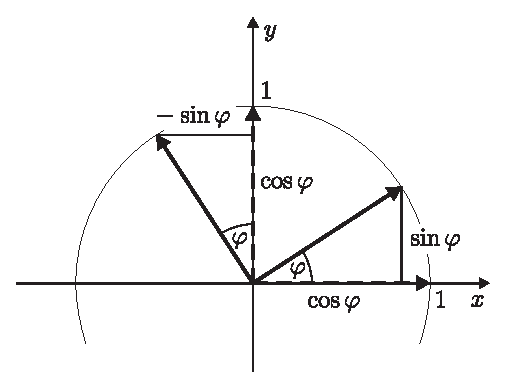
\includegraphics{skript/grafiken/lineare-algebra-2-5-3-a}
    \end{center}
    \begin{itemize}
        \item Definition der Abbildung:
        $$ h \left( \vectwo{x}{y} \right) = \vectwo{x \cdot \cos \varphi - y \cdot \sin \varphi}{x \cdot \sin \varphi + y \cdot \cos \varphi} $$
        \item Abbildung der Basisvektoren:
        $$ \vectwo{1}{0} \mapsto \vectwo{\cos \varphi}{\sin \varphi}, \platz \vectwo{0}{1} \mapsto \vectwo{- \sin \varphi}{\cos \varphi} $$
        \item Matrix:
        $$ C_h = \begin{pmatrix}
          \cos \varphi & - \sin \varphi \\
          \sin \varphi & \cos \varphi
        \end{pmatrix} $$
    \end{itemize}
    \item Drehung ($\circlearrowleft$) von $\real^2$ um einen Winkel $\varphi$ mit anschlie�ender Skalierung um den Faktor $c \in \real$:
    \begin{itemize}
        \item Definition der Abbildung:
        \begin{eqnarray*}
            (f_{\real^2} h) \left( \vectwo{x}{y} \right) &=& f_{\real^2} \left( \vectwo{x \cdot \cos \varphi - y \cdot \sin \varphi}{x \cdot \sin \varphi + y \cdot \cos \varphi} \right) \\ \\
                                                         &=& \vectwo{x \cdot c \cdot \cos \varphi - y \cdot c \cdot \sin \varphi}{x \cdot c \cdot \sin \varphi + y \cdot c \cdot \cos \varphi}
        \end{eqnarray*}
        \item Matrix:
        \begin{eqnarray*}
            A_{f, \real^2} \cdot C_h &=&
            \begin{pmatrix}
            c & 0 \\
            0 & c \\
            \end{pmatrix} \cdot
            \begin{pmatrix}
            \cos \varphi & - \sin \varphi \\
            \sin \varphi & \cos \varphi
            \end{pmatrix} \\ \\
            &=& \begin{pmatrix}
            c \cdot \cos \varphi & - c \cdot \sin \varphi \\
            c \cdot \sin \varphi & c \cdot \cos \varphi
            \end{pmatrix}
        \end{eqnarray*}
    \end{itemize}
\end{enumerate}

%%%%%%%%%%%%%%%%%%%%%%%%%%%%%%%%%%%%%%%%%%%%%%%%%%%%%%%%%%%%%%%%%%%%%%%%%%%%%%%
% Rang einer Matrix
%%%%%%%%%%%%%%%%%%%%%%%%%%%%%%%%%%%%%%%%%%%%%%%%%%%%%%%%%%%%%%%%%%%%%%%%%%%%%%%
\section{Rang einer Matrix}
%%%%%%%%%%%%%%%%%%%%%%%%%%%%%%%%%%%%%%%%%%%%%%%%%%%%%%%%%%%%%%%%%%%%%%%%%%%%%%%
\subsection{Einleitung}

\paragraph{Definition:} Sei $A \in M(m \times n, K)$ eine Matrix und $f \in \text{Hom}(K^n, K^m)$ die zugeh�rige lineare Abbildung (bez�glich der Standardbasis), dann ist der \emph{Rang}\index{Rang einer Matrix} von $A$ definiert als
$$ \text{rg } A := \text{rg } f = \text{dim } (\text{Im } f) $$
Der \emph{Zeilenrang}\index{Zeilenrang} von $A$ ist die maximale Anzahl von linear unabh�ngigen Zeilenvektoren aus $A$. \par \vspace{0.3cm}
Der \emph{Spaltenrang}\index{Spaltenrang} von $A$ ist die maximale Anzahl von linear unabh�ngigen Spaltenvektoren aus $A$.

\paragraph{Lemma:} Ist $\vec{v}_i$ ein Spaltenvektor (Zeilenvektor) von $A$, der sich als Linearkombination der �brigen Spalten (Zeilen) darstellen l�sst und ist $A'$ die Matrix $A$ ohne Spalte (Zeile) $\vec{v}_i$, dann gilt:
$$ \text{Spaltenrang } A' = \text{Spaltenrang } A \platz \text{bzw.} \platz \text{Zeilenrang } A' = \text{Zeilenrang } A $$

\paragraph{Satz:} Der Rang, der Spaltenrang und der Zeilenrang einer Matrix $A$ sind gleich:
$$ \text{rg } A = \text{Spaltenrang } A = \text{Zeilenrang } A $$

\paragraph{Beweis:}
\begin{itemize}
    \item Zu zeigen ist, dass $\text{rg } A = \text{Spaltenrang } A$: \par
    Die Spalten von $A$ sind die Bilder der Basisvektoren. Daraus folgt, dass die Spaltenvektoren Erzeugendensystem f�r $\text{Im } f$ sind. Damit ist die maximale linear unabh�ngige Teilmenge der Spaltenvektoren die Basis von $\text{Im } f$. Also ist der Spaltenrang von $A$ die Dimension von $\text{Im } f$:
    $$ \text{Spaltenrang } A = \text{dim } (\text{Im } f) = \text{rg } A $$
    \item Zu zeigen ist, dass $\text{Spaltenrang } A = \text{Zeilenrang } A$: \par
    Streiche aus $A$ Zeilen und/oder Spalten, die jeweils Linearkombinationen der �brigen Zeilen bzw. Spalten sind, solange das m�glich ist.
    $$ A \mapsto A' \mapsto A'' \mapsto \ldots \mapsto A^{(\text{end})} $$
    Nach dem Lemma gilt:
    \begin{eqnarray*}
        n &:=& \text{Spaltenrang } A = \text{Spaltenrang } A^{(\text{end})} \\
        m &:=& \text{Zeilenrang } A = \text{Zeilenrang } A^{(\text{end})}
    \end{eqnarray*}
    \begin{itemize}
        \item Angenommen, dass $n < m$: \par
        Das hei�t, dass $A^{(\text{end})}$ $m$ Zeilen hat, aber $m$ Vektoren k�nnen in $K^n$ nicht linear unabh�ngig sein. Damit muss einer der Vektoren eine Linearkombination der �brigen Vektoren sein. Dies ist ein Widerspruch zur Annahme. Also ist $n \geq m$.
        \item Angenommen, dass $n > m$: \par
        Das hei�t, dass $A^{(\text{end})}$ $n$ Spalten hat, aber $n$ Vektoren k�nnen in $K^m$ nicht linear unabh�ngig sein. Damit muss einer der Vektoren eine Linearkombination der �brigen Vektoren sein. Dies ist ein Widerspruch zur Annahme. Also ist $n = m$. \hfill $\Box$
    \end{itemize}
\end{itemize}

\paragraph{Definition:} Sei $A = (a_{i \; j}) \in M(m \times n, K)$ eine Matrix, dann ist transponierte Matrix von $A$ definiert durch
$$ A^t = (a_{i \; j}^t) \in M(n \times m, K) \platz \text{mit} \platz a_{i \; j}^t = a_{j \; i} $$

\paragraph{Beispiel:}
$$ \begin{pmatrix} 1 & 0 \\ 2 & 1 \\ 4 & 0 \end{pmatrix}^t = \begin{pmatrix} 1 & 2 & 4 \\ 0 & 1 & 0 \end{pmatrix} $$

\paragraph{Folgerung:} Der Rang einer Matrix $A$ und der transponierten Matrix $A^t$ ist gleich.
$$ \text{rg } A = \text{rg } A^t $$ \pagebreak

%%%%%%%%%%%%%%%%%%%%%%%%%%%%%%%%%%%%%%%%%%%%%%%%%%%%%%%%%%%%%%%%%%%%%%%%%%%%%%%
\subsection{Elementare Umformungen}

\paragraph{Feststellung:} Der Rang einer Matrix kann mit den folgenden elementaren Umformungen bestimmt werden:
\begin{itemize}
    \item Typ 1: Vertauschung von zwei Zeilen (Spalen).
    \item Typ 2: Multiplikation einer Zeile (Spalte) mit einem Skalar $\lambda \neq 0$.
    \item Typ 3: Addition des $\lambda$-fachen einer Zeile (Spalte) zu einer anderen Zeile~(Spalte).
\end{itemize}

\paragraph{Satz:} Elementare Umformungen �ndern den Rang einer Matrix nicht.

\paragraph{Beweis:}
\begin{itemize}
    \item Typ 1 und 2: trivial
    \item Typ 3: Sei $\vec{v}_i$ ein Zeilenvektor vor und $\vec{v}^{\, *}_i$ nach der Umformung, $\vec{v}_k$ sei ein anderer Zeilenvektor und $\lambda \in K$ ein Skalar:
    $$ \vec{v}^{\, *}_i = \vec{v}_i + \lambda \vec{v}_k $$
    Die urspr�ngliche Matrix sei $A$ und die Matrix nach der Umformung $A^*$:
    $$ A^* = A(\vec{v} \leftrightarrow \vec{v}^{\, *}) $$
    Sei $\vec{w}$ darstellbar als Linearkombination aus den Zeilenvektoren von $A$:
    $$ \vec{w} = \mu_1 \vec{v}_1 + \mu_2 \vec{v}_2 + \ldots + \mu_i \vec{v}_i + \ldots + \mu_k \vec{v}_k + \ldots + \mu_n \vec{v}_n $$
    Damit ist der Vektor $\vec{w}$ auch als Linearkombination aus den Zeilenvektoren von $A^*$ darstellbar:
    $$ \vec{w} = \mu_1 \vec{v}_1 + \mu_2 \vec{v}_2 + \ldots + \mu_i \vec{v}^{\, *}_i + \ldots + (\mu_k - \lambda \mu_i) \vec{v}_k + \ldots + \mu_n \vec{v}_n $$
    Daraus folgt:
    $$ \text{Lin}(\text{Zeilenvektoren von $A$}) = \text{Lin}(\text{Zeilenvektoren von $A^*$}) $$
    Da die Dimension gleich bleibt, bleibt auch der Rang gleich. \hfill $\Box$
\end{itemize}

%%%%%%%%%%%%%%%%%%%%%%%%%%%%%%%%%%%%%%%%%%%%%%%%%%%%%%%%%%%%%%%%%%%%%%%%%%%%%%%
%%%%%%%%%%%%%%%%%%%%%%%%%%%%%%%%%%%%%%%%%%%%%%%%%%%%%%%%%%%%%%%%%%%%%%%%%%%%%%%
%%%%%%%%%%%%%%%%%%%%%%%%%%%%%%%%%%%%%%%%%%%%%%%%%%%%%%%%%%%%%%%%%%%%%%%%%%%%%%%
% Bis hier von Herrn Kriegel korrigiert
%%%%%%%%%%%%%%%%%%%%%%%%%%%%%%%%%%%%%%%%%%%%%%%%%%%%%%%%%%%%%%%%%%%%%%%%%%%%%%%
%%%%%%%%%%%%%%%%%%%%%%%%%%%%%%%%%%%%%%%%%%%%%%%%%%%%%%%%%%%%%%%%%%%%%%%%%%%%%%%
%%%%%%%%%%%%%%%%%%%%%%%%%%%%%%%%%%%%%%%%%%%%%%%%%%%%%%%%%%%%%%%%%%%%%%%%%%%%%%%

%%%%%%%%%%%%%%%%%%%%%%%%%%%%%%%%%%%%%%%%%%%%%%%%%%%%%%%%%%%%%%%%%%%%%%%%%%%%%%%
\subsection{Obere Dreiecksform}

\paragraph{Definition:} Die Matrix $A$ ist in oberer Dreiecksform, wenn die Matrix die folgende Form hat (das Symbol $*$ steht f�r beliebigen Inhalt):
$$ A = \left( \begin{array}{ccccc@{\hspace{0.2cm}}|@{\hspace{0.3cm}}ccc}
    a_{1 \, 1} & *          & *          & \cdots & *          & *      & \cdots & *      \\
    0          & a_{2 \, 2} & *          & \cdots & *          & \vdots & \ddots & \vdots \\
    0          & 0          & a_{3 \, 3} & \ddots & \vdots     & \vdots & \ddots & \vdots \\
    \vdots     & \vdots     & \ddots     & \ddots & *          & \vdots & \ddots & \vdots \\
    0          & 0          & \cdots     & 0      & a_{r \, r} & *      & \cdots & *      \\ \hline
    0          & \cdots     & \cdots     & \cdots & 0          & 0      & \cdots & 0      \\
    \vdots     & \ddots     & \ddots     & \ddots & \vdots     & \vdots & \ddots & \vdots \\
    0          & \cdots     & \cdots     & \cdots & 0          & 0      & \cdots & 0
\end{array} \right) $$
F�r die Werte $a_{1 \, 1}, a_{2 \, 2}, a_{3 \, 3}, \ldots a_{r \, r}$ muss dabei gelten:
$$ a_{1 \, 1} \cdot a_{2 \, 2} \cdot a_{3 \, 3} \cdot \ldots \cdot a_{r \, r} \neq 0 $$

\paragraph{Beobachtung:} Der Rang einer solchen Matrix ist $r$.

\paragraph{Verfahren:} �berf�hrung einer Matrix $A \in M(m \times n, K)$ in obere Dreiecksform:
\begin{itemize}
    \item Die Matrix $A_0$ wird mit der Matrix $A$ initialisiert.
    $$ A_0 := A $$
    \item Anschlie�end $A_k$ mit $k = 0, 1, \ldots \min(m, n)$ das folgende Verfahren angewandt. Dabei muss $A_k$ vor jeder Inkrementierung von $k$ folgende Form haben:
    $$ A_k = \left( \begin{array}{ccccc@{\hspace{0.4cm}}|@{\hspace{0.3cm}}ccc}
        a_{1 \, 1} & *          & *          & \cdots & *          & *              & \cdots & *            \\
        0          & a_{2 \, 2} & *          & \cdots & *          & \vdots         & \ddots & \vdots       \\
        0          & 0          & a_{3 \, 3} & \ddots & \vdots     & \vdots         & \ddots & \vdots       \\
        \vdots     & \vdots     & \ddots     & \ddots & *          & \vdots         & \ddots & \vdots       \\
        0          & 0          & \cdots     & 0      & a_{k \, k} & *              & \cdots & *            \\ \hline
        0          & \cdots     & \cdots     & \cdots & 0          & b_{k+1 \; k+1} & \cdots & b_{k+1 \; n} \\
        \vdots     & \ddots     & \ddots     & \ddots & \vdots     & \vdots         & \ddots & \vdots       \\
        0          & \cdots     & \cdots     & \cdots & 0          & b_{m   \; k+1} & \cdots & b_{m   \; n}
    \end{array} \right) $$
    Die Koeffzienten $b_{i \, j}$ (mit $i = k+1, k+2, \ldots m$ und $j = k+1, k+2, \ldots n$) sind beliebig, und es gilt $a_{1 \, 1} \cdot a_{2 \, 2} \cdot a_{3 \, 3} \cdot \ldots \cdot a_{k \, k} \neq 0$. \par
    Die Teilmatrix von $A_k$, die nur aus den Elementen $b_{p \, q}$ besteht, wird im Folgenden mit $B$ bezeichnet:
    $$ B = \begin{pmatrix}
      b_{k+1 \; k+1} & \cdots & b_{k+1 \; n} \\
      \vdots         & \ddots & \vdots       \\
      b_{m   \; k+1} & \cdots & b_{m   \; n} \\
    \end{pmatrix} $$
    Verfahren f�r $A_k$:
    \begin{itemize}
        \item Falls f�r alle $b_{i \, j}$ aus $B$ gilt
        $$ b_{i \, j} = 0 $$
        dann ist das Verfahren abgeschlossen. Die Matrix $A_k$ hat obere Dreiecksform.
        \item Sonst werden folgende Umformungen durchgef�hrt:
        \begin{enumerate} \buchstaben
            \item Vertausche Zeilen und/oder Spalten, die durch $B$ gehen, um einen Koeffizieten $b_{i, j} \neq 0$ an die Stelle $a'_{k+1 \, k+1}$ zu bringen:
            $$ A'_k = \left( \begin{array}{cccc@{\hspace{0.4cm}}|@{\hspace{0.3cm}}cccc}
                a_{1 \, 1} & *          & \cdots & *          & *               & *              & \cdots & *             \\
                0          & a_{2 \, 2} & \ddots & *          & \vdots          & \vdots         & \ddots & \vdots        \\
                \vdots     & \ddots     & \ddots & *          & \vdots          & \vdots         & \ddots & \vdots        \\
                0          & 0          & 0      & a_{k \, k} & *               & *              & \cdots & *             \\ \hline
                0          & \cdots     & \cdots & 0          & a'_{k+1 \; k+1} & \cdots         & \cdots & a'_{k+1 \; n} \\
                \vdots     & \ddots     & \ddots & \vdots     & b'_{k+2 \; k+1} & \cdots         & \cdots & b'_{k+2 \; n} \\
                \vdots     & \ddots     & \ddots & \vdots     & \vdots          & \ddots         & \ddots & \vdots        \\
                0          & \cdots     & \cdots & 0          & b'_{m   \; k+1} & \cdots         & \cdots & b'_{m   \; n}
            \end{array} \right) $$ \pagebreak

            \item F�r $b'_{k+2 \; k+1}, b'_{k+3 \; k+1}, \ldots b'_{m \; k+1}$ werden durch Typ-3-Umformungen Nullen erzeugt:
            $$ A'_k = \left( \begin{array}{cccc@{\hspace{0.4cm}}|@{\hspace{0.3cm}}cccc}
                a_{1 \, 1} & *          & \cdots & *          & *               & *                & \cdots & *              \\
                0          & a_{2 \, 2} & \ddots & *          & \vdots          & \vdots           & \ddots & \vdots         \\
                \vdots     & \ddots     & \ddots & *          & \vdots          & \vdots           & \ddots & \vdots         \\
                0          & 0          & 0      & a_{k \, k} & *               & *                & \cdots & *              \\ \hline
                0          & \cdots     & \cdots & 0          & a'_{k+1 \; k+1} & \cdots           & \cdots & a'_{k+1 \; n}  \\
                \vdots     & \ddots     & \ddots & \vdots     & 0               & b''_{k+2 \; k+2} & \cdots & b''_{k+2 \; n} \\
                \vdots     & \ddots     & \ddots & \vdots     & \vdots          & \vdots           & \ddots & \vdots         \\
                0          & \cdots     & \cdots & 0          & 0               & b''_{m   \; k+2} & \cdots & b''_{m   \; n}
            \end{array} \right) $$
            Dies wird durch folgende Operation realisiert ($i = k+2, k+3, \ldots m$ und $j = k+1, k+2, \ldots n$):
            $$ b''_{i \; j} := b'_{i \; j} - a'_{i \; k+1} \cdot \frac{b'_{k+1 \; j}}{a'_{k+1 \; k+1}} $$
        \end{enumerate}
    \end{itemize}
\end{itemize}

\paragraph{Beispiel:}
\begin{itemize}
    \item Folgende Matrix $A$ soll in obere Dreiecksform umgeformt werden:
    $$ \begin{pmatrix}
      0 & -2 & 4 \\
      2 & 1 & 0 \\
      1 & 0 & 2 \\
      2 & 0 & 3 \\
    \end{pmatrix} $$
    \item Vertausche die erste und die dritte Zeile, so dass an der Stelle $a_{1 \, 1}$ ein Koeffizient $\neq 0$ steht:
    $$ \begin{pmatrix}
      1 & 0 & 2 \\
      2 & 1 & 0 \\
      0 & -2 & 4 \\
      2 & 0 & 3 \\
    \end{pmatrix} $$
    \item Erzeuge an den Stellen $a_{2 \; 1}$ und $a_{4 \; 1}$ Nullen durch Typ-3-Umformungen mit der ersten Zeile:
    $$ \begin{pmatrix}
      1 & 0 & 2 \\
      2 - 1 \cdot 2 & 1 - 0 \cdot 2 & 0 - 2 \cdot 2 \\
      0 & -2 & 4 \\
      2 - 1 \cdot 2 & 0 - 0 \cdot 2 & 3 - 2 \cdot 2 \\
    \end{pmatrix} =
    \begin{pmatrix}
      1 & 0 & 2 \\
      0 & 1 & -4 \\
      0 & -2 & 4 \\
      0 & 0 & -1 \\
    \end{pmatrix} $$
    \item An der Stelle $a_{2 \, 2}$ befindet sich ein Koeffizient $\neq 0$. Damit muss nur noch an der Stelle $a_{2 \, 3}$ eine Null erzeugt werden:
    $$ \begin{pmatrix}
      1 & 0 & 2 \\
      0 & 1 & -4 \\
      0 & -2 - (-2) \cdot 1 & 4 - (-2) \cdot (-4) \\
      0 & 0 & -1 \\
    \end{pmatrix} =
    \begin{pmatrix}
      1 & 0 & 2 \\
      0 & 1 & -4 \\
      0 & 0 & -4 \\
      0 & 0 & -1 \\
    \end{pmatrix} $$
    \item An der Stelle $a_{3 \, 3}$ muss eine Null erzeugt werden:
    $$ \begin{pmatrix}
      1 & 0 & 2 \\
      0 & 1 & -4 \\
      0 & 0 & -4 \\
      0 & 0 & -1 - \frac{1}{4} \cdot (-4) \\
    \end{pmatrix} =
    \begin{pmatrix}
      1 & 0 & 2 \\
      0 & 1 & -4 \\
      0 & 0 & -4 \\
      0 & 0 & 0 \\
    \end{pmatrix} $$
\end{itemize}

%%%%%%%%%%%%%%%%%%%%%%%%%%%%%%%%%%%%%%%%%%%%%%%%%%%%%%%%%%%%%%%%%%%%%%%%%%%%%%%
\subsection{Elementarmatrizen}

\paragraph{Beobachtung:} Elementare Matrixumformungen k�nnen auch durch Multiplikation mit sogenannten Elementarmatrizen realisiert werden.
\begin{itemize}
    \item Typ 1: \par
    F�r die Vertauschung der $i$-ten und der $j$-ten Zeile (Spalte) in einer Matrix $A$ wird folgende Matrix durch Abwandlung der Einheitsmatrix konstruiert:
    $$ T_{i \, j} = \left( \begin{array}{cccccccccccc}
        1      &        &        &            &        &             &        &          &        &        &          \\
               & \ddots &        &            &        &             &        &          &        & 0      &          \\
               &        & 1      &            &        &             &        &          &        &        &          \\
               &        &        & 0          & \cdots & \rightarrow & \cdots & 1        &        &        &          \\
               &        &        & \vdots     & 1      &             &        & \vdots   &        &        &          \\
               &        &        & \downarrow &        & \ddots      &        & \uparrow &        &        &          \\
               &        &        & \vdots     &        &             & 1      & \vdots   &        &        &          \\
               &        &        & 1          & \cdots & \leftarrow  & \cdots & 0        &        &        &          \\
               &        &        &            &        &             &        &          & 1      &        &          \\
               & 0      &        &            &        &             &        &          &        & \ddots &          \\
               &        &        &            &        &             &        &          &        &        & 1        \\
    \end{array} \right) \begin{array}{ll}
      \longleftarrow & \text{$i$-te Zeile} \\
      \ \\
      \ \\
      \ \\
      \ \\
      \longleftarrow & \text{$j$-te Zeile} \\
    \end{array} $$
    Vertauschung der $i$-ten und der $j$-ten Zeile:
    $$ A' =  T_{i \, j} \cdot A $$
    Vertauschung der $i$-ten und der $j$-ten Spalte:
    $$ A'' = A \cdot T_{i \, j} $$

    \item Typ 2: \par
    F�r die Multiplikation einer Zeile (Spalte) mit dem Faktor $\lambda$ in einer Matrix $A$ wird eine Matrix konstruiert, in welcher in der Diagonalen der Einheitsmatrix in der entsprechenden Zeile (Spalte) eine Eins durch $\lambda$ ersetzt:
    $$ S_{i \, \lambda} = \left( \begin{array}{ccccccc}
        1     &        &        &         &        &        &        \\
              & \ddots &        &         &        & 0      &        \\
              &        & 1      &         &        &        &        \\
              &        &        & \lambda &        &        &        \\
              &        &        &         & 1      &        &        \\
              & 0      &        &         &        & \ddots &        \\
              &        &        &         &        &        & 1      \\
    \end{array} \right) \begin{array}{ll}
      \longleftarrow & \text{$i$-te Zeile} \\
    \end{array} $$
    Multiplkation der $i$-ten Zeile mit $\lambda$:
    $$ A' =  S_{i \, \lambda} \cdot A $$
    Multiplkation der $j$-ten Spalte mit $\lambda$:
    $$ A'' = A \cdot S_{i \, \lambda} $$

    \item Typ 3: \par
    F�r die Addition des $\lambda$-fachen einer Zeile (Spalte) zu einer anderen Zeile (Spalte) in einer Matrix $A$ wird eine Einheitsmatrix um ein $\lambda$ folgenderma�en erweitert:
    $$ \begin{array}{c}
        K_{i \, j \, \lambda} = \left( \begin{array}{ccccccc}
        1     &        &        &        &         &        &        \\
              & \ddots &        &        &         & 0      &        \\
              &        & \ddots &        &         &        &        \\
              &        &        & \ddots & \lambda &        &        \\
              &        &        &        & \ddots  &        &        \\
              & 0      &        &        &         & \ddots &        \\
              &        &        &        &         &        & 1      \\
        \end{array} \right) \begin{array}{ll}
            \longleftarrow & \text{$i$-te Zeile} \\
        \end{array} \\
        \uparrow \\
        \text{$j$-te Spalte} \\
    \end{array} $$
    Addition des $\lambda$-fachen der $j$-ten Zeile zur $i$-ten Zeile:
    $$ A' =  K_{i \, j \, \lambda} \cdot A $$
    Addition des $\lambda$-fachen der $i$-ten Spalte zur $j$-ten Spalte:
    $$ A'' = A \cdot K_{i \, j \, \lambda} $$
\end{itemize}

%%%%%%%%%%%%%%%%%%%%%%%%%%%%%%%%%%%%%%%%%%%%%%%%%%%%%%%%%%%%%%%%%%%%%%%%%%%%%%%
% Lineare Gleichungssysteme
%%%%%%%%%%%%%%%%%%%%%%%%%%%%%%%%%%%%%%%%%%%%%%%%%%%%%%%%%%%%%%%%%%%%%%%%%%%%%%%
\section{Lineare Gleichungssysteme}
%%%%%%%%%%%%%%%%%%%%%%%%%%%%%%%%%%%%%%%%%%%%%%%%%%%%%%%%%%%%%%%%%%%%%%%%%%%%%%%
\subsection{Einleitung}

\paragraph{Definition:} Ein \emph{lineares Gleichungssystem}\index{lineares Gleichungssystem}\index{Gleichungssystem, linear} (LGS)\index{LGS} mit Koeffizienten in einem K�rper $K$, mit $m$ Gleichungen und $n$ Unbekannten wird durch eine Matrix
$$ A = (a_{i \, j})_{(i, j) \in m \times n} \in M(m \times n, K) $$
und einem Vektor
$$ \vec{b} = \begin{pmatrix}
  b_1 \\
  b_2 \\
  \vdots \\
  b_m
\end{pmatrix} \in K^m $$
repr�sentiert. Das lineare Gleichungssystem  wird folgenderma�en interpretiert:
$$ \begin{array}{ccccccccc}
  a_{1 \, 1} \cdot x_1 & + & a_{1 \, 2} \cdot x_2 & + & \ldots & + & a_{1 \, n} \cdot x_n & = & b_1    \\
  a_{2 \, 1} \cdot x_1 & + & a_{2 \, 2} \cdot x_2 & + & \ldots & + & a_{2 \, n} \cdot x_n & = & b_2    \\
  \vdots               &   & \vdots               &   &        &   & \vdots               &   & \vdots \\
  a_{m \, 1} \cdot x_1 & + & a_{m \, 2} \cdot x_2 & + & \ldots & + & a_{m \, n} \cdot x_n & = & b_m    \\
\end{array} $$

Man bezeichnet mit $(A \, | \, b)$ folgende Matrix:
$$ (A \, | \, b) = \left( \begin{array}{cccc|c}
    a_{1 \, 1} & a_{1 \, 2} & \cdots & a_{1 \, n} & b_1 \\
    a_{2 \, 1} & a_{2 \, 2} & \cdots & a_{2 \, n} & b_2 \\
    \vdots     & \vdots     & \ddots & \vdots           \\
    a_{m \, 1} & a_{m \, 2} & \cdots & a_{m \, n} & b_m \\
\end{array} \right) $$

\paragraph{Beobachtung:} $x_1, x_2, \ldots x_n$ bilden genau dann eine L�sung des linearen Gleichungssystems, wenn
$$ A \cdot \begin{pmatrix}
  x_1 \\
  x_2 \\
  \vdots \\
  x_n
\end{pmatrix} = \vec{b} $$ \pagebreak

\paragraph{Satz:} Die Gleichung $A \cdot \vec{x} = \vec{b}$ ist genau dann l�sbar, wenn
$$ \text{rg } A = \text{rg}(A \, | \, b) $$

\paragraph{Beweis:}
\begin{eqnarray*}
    &               & \text{rg } A = \text{rg}(A \; | \; b) \\ \\
    &\Leftrightarrow& \text{Spaltenrang}(A) = \text{Spaltenrang}(A \; | \; b) \\ \\
    &\Leftrightarrow& \vec{b} \in \text{Lin} \left( \left\{ \vecfour{a_{1 \, 1}}{a_{2 \, 1}}{\vdots}{a_{m \, 1}}, \vecfour{a_{1 \, 2}}{a_{2 \, 2}}{\vdots}{a_{m \, 2}}, \ldots \vecfour{a_{1 \, n}}{a_{2 \, n}}{\vdots}{a_{m \, n}} \right\} \right) \\ \\
    &\Leftrightarrow& \exists x_1, x_2, \ldots x_n \platz \vec{b} = x_1 \cdot \vecfour{a_{1 \, 1}}{a_{2 \, 1}}{\vdots}{a_{m \, 1}} + x_2 \cdot \vecfour{a_{1 \, 2}}{a_{2 \, 2}}{\vdots}{a_{m \, 2}} + \ldots + x_n \cdot \vecfour{a_{1 \, n}}{a_{2 \, n}}{\vdots}{a_{m \, n}} \\ \\
    &\Leftrightarrow& \exists x_1, x_2, \ldots x_n \platz A \cdot \vecfour{x_1}{x_2}{\vdots}{x_n} = \vec{b}
\end{eqnarray*}

\paragraph{Definition:} Ein lineares Gleichungssystem mit $\vec{b} = \vec{0}^{\; (m)}$ wird \emph{homogenes Gleichungssystem}\index{homogenes Gleichungssystem}\index{Gleichungssystem, homogen} genannt.

\paragraph{Beobachtung:} Zu jedem linearen Gleichungssystem kann durch Ersetzung von~$\vec{b}$ durch $\vec{0}^{\; (m)}$ ein homogenes Gleichungssystem gefunden werden.

\paragraph{Definition:} Die L�sungsmenge eines linaren Gleichungssystems aus $A$ und $\vec{b}$ ist folgerma�en definiert:
$$ \text{L�s}(A, \vec{b}) = \{ \vec{x} \; | \; A \cdot \vec{x} = \vec{b} \} $$

\paragraph{Satz:} Sei $A \in M(m \times n, K)$ die Matrix einer linearen Abbildung $f : K^n \rightarrow K^m$ bez�glich der Standardbasis, dann ist
\begin{enumerate} \buchstaben
    \item Die L�sungsmenge $\text{L�s}(A, \vec{0}^{\; (m)})$ ist gleich $\text{Ker } f$. Damit ist $\text{L�s}(A, \vec{0}^{\; (m)})$ ein Unterraum von $K^n$.
    \item Sei $\vec{b} \in K^m$ und $\vec{x}, \vec{y} \in \text{L�s}(A, \vec{b})$, dann gilt:
    $$ \vec{x} - \vec{y} \in \text{L�s}(A, \vec{0}^{\; (m)}) $$
    \item Sei $\vec{b} \in K^m$, $\vec{x} \in \text{L�s}(A, \vec{b})$ und $\vec{z} \in \text{L�s}(A, \vec{0}^{\; (m)})$, dann gilt:
    $$ \vec{x} + \vec{z} \in \text{L�s}(A, \vec{b}) $$
\end{enumerate}

\paragraph{Beweis:}
\begin{enumerate} \buchstaben
    \item Durch Einsetzen der jeweiligen Definitionen folgt:
    \begin{eqnarray*}
        \text{L�s}(A, \vec{0}^{\; (m)}) &=& \{ \vec{x} \; | \; A \cdot \vec{x} = \vec{0}^{\; (m)} \} \\
                                        &=& \{ \vec{x} \; | \; f(\vec{x}) = \vec{0}^{\; (m)} \} \\
                                        &=& \text{Ker } f
    \end{eqnarray*}
    \item Seien $\vec{x}, \vec{y} \in \text{L�s}(A, \vec{b})$, dann gilt:
    $$ f(\vec{x}) = \vec{b} \platz \text{und} \platz f(\vec{y}) = \vec{b} $$
    Daraus folgt:
    $$ f(\vec{x} - \vec{y}) = f(\vec{x}) - f(\vec{y}) = \vec{b} - \vec{b} = \vec{0} $$
    Das hei�t:
    $$ \vec{x} - \vec{y} \in \text{L�s}(A, \vec{0}^{\; (m)}) $$
    \item Seien $\vec{x} \in \text{L�s}(A, \vec{b})$ und $\vec{z} \in \text{L�s}(A, \vec{0}^{\; (m)})$, dann gilt:
    $$ f(\vec{x}) = \vec{b} \platz \text{und} \platz f(\vec{z}) = \vec{0} $$
    Daraus folgt:
    $$ f(\vec{x} + \vec{z}) = f(\vec{x}) - f(\vec{z}) = \vec{b} - \vec{0} = \vec{b} $$
    Das hei�t:
    $$ \vec{x} + \vec{z} \in \text{L�s}(A, \vec{b}) $$
\end{enumerate}

\paragraph{Beobachtung:} Sei $A \in M(m \times n, K)$ die Matrix einer linearen Abbildung $f : K^n \rightarrow K^m$ bez�glich der Standardbasis, dann ist die L�sungsmenge $\text{L�s}(A, b)$ genau dann \emph{nicht} leer, wenn $\vec{b} \in \text{Im } f$.

%%%%%%%%%%%%%%%%%%%%%%%%%%%%%%%%%%%%%%%%%%%%%%%%%%%%%%%%%%%%%%%%%%%%%%%%%%%%%%%
\subsection{Gau�'scher Algorithmus}\index{Gau�'scher Algorithmus}

\paragraph{Verfahren:} Ein lineares Gleichungssystem aus $A$ und $\vec{b}$ kann nach folgendem Algorithmus gel�st werden:
\begin{enumerate} \buchstaben
    \item �berpr�fung, ob das lineare Gleichungssystem eine L�sung hat:
    Man bringt die Matrix $A$ in obere Dreiecksform, aber erweitert alle Schritte auf die Matrix $(A \; | \; b)$ ohne Elementarumformungen mit letzter Spalte vorzunehmen. \par
    Achtung: Spaltenvertauschungen in $A$ bedeuten Variablenvertauschung im linearen Gleichungssystem. \par
    Ergebnis:
    $$ A' = \left( \begin{array}{ccccc@{\hspace{0.2cm}}|@{\hspace{0.3cm}}ccc@{\hspace{0.4cm}}|c}
        a'_{1 \, 1} & *           & *           & \cdots & *           & *      & \cdots & *      & b'_1     \\
        0           & a'_{2 \, 2} & *           & \cdots & *           & \vdots & \ddots & \vdots & b'_2     \\
        0           & 0           & a'_{3 \, 3} & \ddots & \vdots      & \vdots & \ddots & \vdots & b'_3     \\
        \vdots      & \vdots      & \ddots      & \ddots & *           & \vdots & \ddots & \vdots & \vdots   \\
        0           & 0           & \cdots      & 0      & a'_{r \, r} & *      & \cdots & *      & b'_r     \\ \hline
        0           & \cdots      & \cdots      & \cdots & 0           & 0      & \cdots & 0      & b'_{r+1} \\
        \vdots      & \ddots      & \ddots      & \ddots & \vdots      & \vdots & \ddots & \vdots & \vdots   \\
        0           & \cdots      & \cdots      & \cdots & 0           & 0      & \cdots & 0      & b'_m
    \end{array} \right) $$
    \begin{itemize}
        \item Fall 1: Falls mindestens ein $b'_i \neq 0$ mit $i = r+1, r+2, \ldots m$ existiert, dann ist $\text{rg } (A) < \text{rg} (A \; | \; b)$, und das System hat \emph{keine} L�sung. Das Verfahren wird abgebrochen.
        \item Fall 2: Falls $b'_{r+1} = b'_{r+2} = \ldots = b'_m = 0$, dann ist $\text{rg } (A) = \text{rg} (A \; | \; b)$, und das System hat eine L�sung. \par
        Im Folgenden wird das System auf folgende Form reduziert:
        $$ (T \; | \; S \; | \; b') = \left( \begin{array}{ccccc@{\hspace{0.2cm}}|@{\hspace{0.3cm}}ccc@{\hspace{0.4cm}}|c}
            a'_{1 \, 1} & *           & *           & \cdots & *           & *      & \cdots & *      & b'_1     \\
            0           & a'_{2 \, 2} & *           & \cdots & *           & \vdots & \ddots & \vdots & b'_2     \\
            0           & 0           & a'_{3 \, 3} & \ddots & \vdots      & \vdots & \ddots & \vdots & b'_3     \\
            \vdots      & \vdots      & \ddots      & \ddots & *           & \vdots & \ddots & \vdots & \vdots   \\
            0           & 0           & \cdots      & 0      & a'_{r \, r} & *      & \cdots & *      & b'_r
        \end{array} \right) $$
    \end{itemize} \pagebreak

    \item Bestimmung einer speziellen L�sung von $(T \; | \; S \; | \; b')$: \par
    Zur Bestimmung \emph{einer} speziellen L�sung von $(T \; | \; S \; | \; b')$ wird das lineare Gleichungssystem folgenderma�er geteilt:
    $$ (T \; | \; S) \cdot \begin{pmatrix} x_1 \\ x_2 \\ \vdots \\ x_r \\ x_{r+1} \\ \vdots \\ x_n \end{pmatrix} = T \cdot \vecfour{x_1}{x_2}{\vdots}{x_r} + S \cdot \vecfour{x_{r+1}}{x_{r+2}}{\vdots}{x_n} = \vec{b}' $$
    Man w�hlt $x_{r+1} = x_{r+2} = \ldots = x_n = 0$. Dadurch reduziert sich das lineare Gleichungssystem wiefolgt:
    $$ T \cdot \vecfour{x_1}{x_2}{\vdots}{x_r} = \vec{b}' \platz \Rightarrow \platz \left( \begin{array}{ccccc}
            a'_{1 \, 1} & a'_{1 \, 2} & \cdots & a'_{1 \, r} \\
            0           & a'_{2 \, 2} & \cdots & a'_{2 \, r} \\
            \vdots      & \ddots      & \ddots & \vdots      \\
            0           & \cdots      & 0      & a'_{r \, r}
    \end{array} \right) \cdot \vecfour{x_1}{x_2}{\vdots}{x_r} = \vecfour{b'_1}{b'_2}{\vdots}{b'_r} $$
    Die Werte von $x_1, x_2, \ldots x_r$ k�nnen nun direkt bestimmt werden:
    $$ \begin{array}{rcl@{\hspace{0.5cm}}c@{\hspace{0.5cm}}rcl}
        b'_r     &=& a'_{r \, r}     \cdot x_r                               &\Rightarrow& x_r     &=& \frac{b'_r}{a'_{r \, r}}                                            \\ \\
        b'_{r-1} &=& a'_{r-1 \, r-1} \cdot x_{r-1} +          a'_{r-1 \, r} \cdot x_r &\Rightarrow& x_{r-1} &=& \frac{b'_{r-1} - a'_{r-1 \, r} \cdot x_r}{a'_{r-1 \, r-1}} \\ \\
                 & &                                                                  &\vdots     &         & &                                                            \\ \\
        b'_1     &=& a'_{1 \, 1}     \cdot x_1     + \ldots + a'_{1 \, r}   \cdot x_r &\Rightarrow& x_1     &=& \frac{b'_1     - a'_{1 \, r}   \cdot x_r - \ldots - a'_{1 \, 2} \cdot x_2}{a'_{1 \, 1}} \\ \\
    \end{array} $$
    Der Vektor mit einer speziellen L�sung des linearen Gleichungssystem werde mit $\vec{x}$ bezeichnet:
    $$ \vec{x} = \begin{pmatrix} x_1 \\ x_2 \\ \vdots \\ x_r \\ x_{r+1} \\ \vdots \\ x_n \end{pmatrix} = \begin{pmatrix} x_1 \\ x_2 \\ \vdots \\ x_r \\ 0 \\ \vdots \\ 0 \end{pmatrix} $$ \pagebreak

    \item Bestimmung einer Basis der L�sungsmenge des homogenen Gleichungssystems $(T \; | \; S \; | \; \vec{0}^{\; (r)})$: \par
    Zur Bestimmung des $j$-ten Basisvektors von
    $$ (T \; | \; S) \cdot \begin{pmatrix} x_1 \\ x_2 \\ \vdots \\ x_r \\ x_{r+1} \\ \vdots \\ x_n \end{pmatrix} = T \cdot \vecfour{x_1}{x_2}{\vdots}{x_r} + S \cdot \vecfour{x_{r+1}}{x_{r+2}}{\vdots}{x_n} = \vec{0}^{\; (r)} $$
    w�hlt man
    $$ x_{r+j} = 1 \platz \text{und} \platz x_{r+1} = \ldots = x_{r+j-1} = x_{r+j+1} = \ldots x_n = 0 $$
    Im Folgenden gelte:
    $$ S = (s_{i \; j})_{(i, j) \in r \times (n-r)} $$
    Damit erh�lt man das folgende lineare Gleichungssystem
    $$ \left( \begin{array}{ccccc}
            a'_{1 \, 1} & a'_{1 \, 2} & \cdots & a'_{1 \, r} \\
            0           & a'_{2 \, 2} & \cdots & a'_{2 \, r} \\
            \vdots      & \ddots      & \ddots & \vdots      \\
            0           & \cdots      & 0      & a'_{r \, r}
    \end{array} \right) \cdot \vecfour{x_1}{x_2}{\vdots}{x_r} = \vecfour{- s_{1 \; j}}{- s_{2 \; j}}{\vdots}{- s_{r \; j}} $$
    Bemerkung: Der Vektor
    $$ \vecfour{- s_{1 \; j}}{- s_{2 \; j}}{\vdots}{- s_{r \; j}} $$
    ist dabei der $j$-Spaltenvektor aus $S$, multipliziert mit $-1$. \par \vspace{0.3cm}
    Die Werte von $x_1, x_2, \ldots x_r$ k�nnen nun wie bei der speziellen L�sung bestimmt werden. \par \vspace{0.3cm}
    Der $j$-te Basisvektor des homogenen Gleichungssystem werde mit $\vec{x}_j$ bezeichnet. \par \vspace{0.3cm}
    Das Verfahren muss f�r alle $n-r$ Spalten von $S$ durchgef�hrt werden. \pagebreak

    \item Bestimmung der allgemeinen L�sung von $(T \; | \; S \; | \; b)$: \par
    Mit Hilfe der speziellen L�sung des linaren Gleichungssystem und der Basisvektoren der L�sungsmenge der homogenen Gleichungssystem l�sst sich die L�sungsmenge des linearen Gleichungssystem folgerma�en darstellen:
    $$ \text{L�s}(A \; | \; b) = \text{L�s}(T \; | S \; | \; b') = \left\{ \vec{x} + \sum_{j=1}^{n-r} \lambda_j \cdot \vec{x}_j \; | \; \lambda_1, \lambda_2, \ldots \lambda_{n-r} \in \real \right\} $$
\end{enumerate}

\paragraph{Beispiel:} Gegeben sei das folgende Gleichungssystem:
$$ \begin{array}{rrrrrrrrrr}
    &   &   & 2x_2 & + & x_3 & - & x_4 & = & 6 \\
    & x_1 & - & x_2 & + & 2x_3 &   &   & = & -1 \\
    & 2x_1 &   &   & + & 5x_3 &   &   & = & 3 \\
  - & x_1 & - & x_2 & - & 3x_3 & + & 2x_4 & = & -6 \\
\end{array} $$
\begin{enumerate} \buchstaben
    \item Die dazugeh�rige Matrix $(A \; | \; b)$:
    $$ \left( \begin{array}{rrrr|r}
        0 & 2 & 1 & -1 & 6 \\
        1 & -1 & 2 & 0 & -1 \\
        2 & 0 & 5 & 0 & 3 \\
        -1 & -1 & -3 & 2 & -6 \\
    \end{array} \right) $$
    Diese Matrix muss zuerst in obere Dreiecksform �berf�hrt werden. \par
    Erste und zweite Zeile vertauschen:
    $$ \left( \begin{array}{rrrr|r}
        1 & -1 & 2 & 0 & -1 \\
        0 & 2 & 1 & -1 & 6 \\
        2 & 0 & 5 & 0 & 3 \\
        -1 & -1 & -3 & 2 & -6 \\
    \end{array} \right) $$
    In der ersten Spalte unter $a_{1 \; 1}$ Nullen erzeugen:
    $$ \left( \begin{array}{rrrr|r}
        1 & -1 & 2 & 0 & -1 \\
        0 & 2 & 1 & -1 & 6 \\
        0 & 2 & 1 & 0 & 5 \\
        0 & -2 & -1 & 2 & -7 \\
    \end{array} \right) $$
    In der zweiten Spalte unter $a_{2 \; 2}$ Nullen erzeugen:
    $$ \left( \begin{array}{rr@{\hspace{0.65cm}}rr|r}
        1 & -1 & 2 & 0 & -1 \\
        0 & 2 & 1 & -1 & 6 \\
        0 & 0 & 0 & 1 & -1 \\
        0 & 0 & 0 & 1 & -1 \\
    \end{array} \right) $$
    Dritte und vierte Spalte tauschen, um an der Stelle $a_{3 \; 3}$ einen Wert $\neq 0$ zu erzeugen (Achtung: $x_3 \leftrightarrow x_4$):
    $$ \left( \begin{array}{rrr@{\hspace{0.65cm}}r|r}
        1 & -1 & 0 & 2 & -1 \\
        0 & 2 & -1 & 1 & 6 \\
        0 & 0 & 1 & 0 & -1 \\
        0 & 0 & 1 & 0 & -1 \\
    \end{array} \right) $$
    In der dritten Spalte unter $a_{3 \; 3}$ Nullen erzeugen:
    $$ \left( \begin{array}{rrr@{\hspace{0.3cm}}|@{\hspace{0.3cm}}r|r}
        1 & -1 & 0 & 2 & -1 \\
        0 & 2 & -1 & 1 & 6 \\
        0 & 0 & 1 & 0 & -1 \\ \hline
        0 & 0 & 0 & 0 & 0 \\
    \end{array} \right) $$
    Die Matrix hat nun obere Dreiecksform. \par
    Es existiert eine L�sung, da der untere Teil von $\vec{b}$ aus einer Null besteht. Die Matrix kann nun folgenderma�en reduziert werden:
    $$ \left( \begin{array}{rrr@{\hspace{0.3cm}}|@{\hspace{0.3cm}}r|r}
        1 & -1 & 0 & 2 & -1 \\
        0 & 2 & -1 & 1 & 6 \\
        0 & 0 & 1 & 0 & -1 \\
    \end{array} \right) $$
    Das lineare Gleichungssystem wird geteilt:
    $$ \left( \begin{array}{rrr}
        1 & -1 & 0 \\
        0 & 2 & -1 \\
        0 & 0 & 1  \\
    \end{array} \right) \cdot \vecthree{x_1}{x_2}{x_4} + \vecthree{2}{1}{0} \cdot \left( x_3 \right) = \left( \begin{array}{r} -1 \\ 6 \\ -1 \\ \end{array} \right) $$

    \item Bestimmung der speziellen L�sung:
    $$ \left( \begin{array}{rrr}
        1 & -1 & 0 \\
        0 & 2 & -1 \\
        0 & 0 & 1  \\
    \end{array} \right) \cdot \vecthree{x_1}{x_2}{x_4} = \left( \begin{array}{r} -1 \\ 6 \\ -1 \\ \end{array} \right) $$
    W�hle $x_3 = 0$ und bestimme die �brigen Variablen:
    $$ \begin{array}{rcrcrcr@{\hspace{0.5cm}}c@{\hspace{0.5cm}}rcr}
                    & &                & &    1 \cdot x_4 &=& -1 &\Rightarrow& x_4 &=&  -1 \\
                    & &    2 \cdot x_2 &+& (-1) \cdot x_4 &=&  6 &\Rightarrow& x_2 &=& 2,5 \\
        1 \cdot x_1 &+& (-1) \cdot x_2 &+&    0 \cdot x_4 &=& -1 &\Rightarrow& x_1 &=& 1,5
    \end{array} $$ \pagebreak

    \item Bestimmung des ersten (und einzigen) Basisvektors von $(A \; | \; \vec{0}^{\; (4)})$:
    $$ \left( \begin{array}{rrr}
        1 & -1 & 0 \\
        0 & 2 & -1 \\
        0 & 0 & 1  \\
    \end{array} \right) \cdot \vecthree{x_1}{x_2}{x_4} = \left( \begin{array}{r} -2 \\ -1 \\ 0 \\ \end{array} \right) $$
    W�hle $x_3 = 1$ und bestimme die �brigen Variablen:
    $$ \begin{array}{rcrcrcr@{\hspace{0.5cm}}c@{\hspace{0.5cm}}rcr}
                    & &                & &    1 \cdot x_4 &=&  0 &\Rightarrow& x_4 &=&    0 \\
                    & &    2 \cdot x_2 &+& (-1) \cdot x_4 &=& -1 &\Rightarrow& x_2 &=& -0,5 \\
        1 \cdot x_1 &+& (-1) \cdot x_2 &+&    0 \cdot x_4 &=& -2 &\Rightarrow& x_1 &=& -2,5
    \end{array} $$
    \item L�sungsmenge:
    $$ \text{L�s}(A \; | \; b) = \left\{ \vecfour{1,5}{2,5}{0}{-1} + \lambda \cdot \vecfour{-2,5}{-0,5}{1}{0} \; | \; \lambda \in \real \right\} $$
\end{enumerate}

%%%%%%%%%%%%%%%%%%%%%%%%%%%%%%%%%%%%%%%%%%%%%%%%%%%%%%%%%%%%%%%%%%%%%%%%%%%%%%%
\subsection{Quotientenraum}

\paragraph{Beobachtung:} Die L�sungsmenge ist \emph{kein} Unterraum, aber eine "`Verschiebung"' eines Unterraums.

\paragraph{Definition:} Sei $V$ ein Vektorraum, $U$ ein Unterraum von $V$ und $\vec{v}$ ein Vektor aus $V$, dann nennt man
$$ \vec{v} + U = \{ \vec{v} + \vec{u} \; | \; \vec{u} \in U \} $$
die \emph{Nebenklasse}\index{Nebenklasse} von $\vec{v}$ bez�glich $U$.

\paragraph{Satz:} Sei $V$ ein Vektorraum, $U$ ein Unterraum von $V$ und $\vec{w}, \vec{w}$ zwei Vektoren aus $V$, dann gilt:
$$ \vec{v} + U = \vec{w} + U \platz \Leftrightarrow \platz \vec{v} - \vec{w} \in U \platz \Leftrightarrow \platz \vec{w} \in \vec{v} + U $$

\paragraph{Definition:} Sei $V$ ein Vektorraum, $U$ ein Unterraum von $V$ und $K$ der K�rper von $V$, dann bezeichnet man die Menge
$$ V_{/ U} = \{ \vec{v} + U \; | \; \vec{v} \in V \} $$
als \emph{Quotientenraum}\index{Quotientenraum} von $V$ nach $U$. \pagebreak[3]

\paragraph{Beobachtung:} Der Quotientenraum $V_{/ U}$ ist ein Vektorraum mit folgenden Operationen ($\vec{v}, \vec{w} \in V$, $\lambda \in K$)
\begin{eqnarray*}
    (\vec{v} + U) + (\vec{w} + U) &=& (\vec{v} + \vec{w}) + U \\
    \lambda \cdot (\vec{v} + U) &=& (\lambda \cdot \vec{v}) + U
\end{eqnarray*}
\begin{center}
    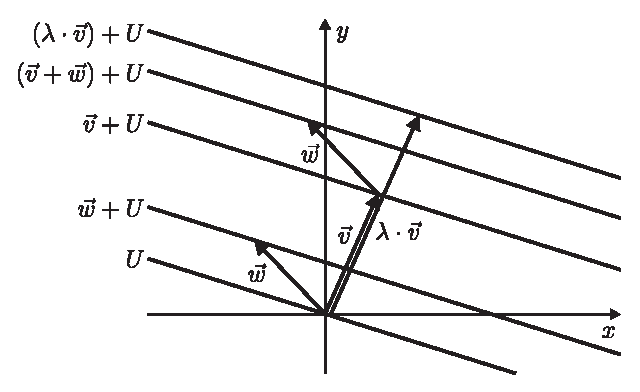
\includegraphics{skript/grafiken/lineare-algebra-2-7-3-a}
\end{center}
und dem neutralen Element $\vec{0} + U = U$.


\paragraph{Beobachtung:} Sei $V_{/ U}$ ein Quotientenraum, dann ist $\vec{v} + U \in V_{/ U}$ eine �quivalenzklasse von $\vec{v}$ bez�glich der Relation "`Differenz ist in $U$"'.

\paragraph{Satz:} Sei $V$ ein Vektorraum, $U$ ein Unterraum von $V$, dann ist
$$ \text{dim } V_{/ U} = \text{dim } V - \text{dim } U $$

\paragraph{Beweisidee:} Man definiert eine Abbildung $\varphi : V \rightarrow V_{/ U}$ durch
$$ \vec{v} \mapsto \vec{v} + U $$
Die Abbidlung $\varphi$ ist linear und surjektiv (epimorph). Damit ist das $\text{Im } \varphi = V_{/ U}$. Au�erdem ist $\text{Ker } \varphi = U$, denn
$$ \forall \, \vec{v} \in U \platz \vec{v} + U = U = \vec{0} + U $$
Nach der Dimensionsformel gilt somit:
$$ \text{dim } V = \text{dim}(\text{Ker } \varphi) + \text{dim} (\text{Im } \varphi) = \text{dim } U + \text{dim } V_{/ U} $$

\paragraph{Beobachtung:} Seien $A \in M(m \times n, K)$ eine Matrix, $f \in \text{Hom}(K^n, K^m)$ die dazugeh�rige Abbildung, $\vec{b}, \vec{c} \in K^n$ sowie $\vec{x}, \vec{y} \in K^m$ Vektoren und $\lambda \in K$ ein Skalar.
\begin{itemize}
    \item Addition:
    $$ \begin{array}{c}
        \text{L�s}(A, \vec{b} + \vec{c}) = (\vec{x} + \vec{y}) + \text{Ker } f \\ \\
        \Updownarrow \\ \\
        \text{L�s}(A, \vec{b}) = \vec{x} + \text{Ker } f \platz \text{und} \platz \text{L�s}(A, \vec{c}) = \vec{y} + \text{Ker } f
    \end{array} $$
    \item Multiplikation mit Skalaren:
    $$ \begin{array}{c}
        \text{L�s}(A \, | \, \vec{b}) = \vec{x} + \text{Ker } f \\ \\
        \Updownarrow \\ \\
        \text{L�s}(A \, | \, \lambda \, \vec{b}) = \lambda \, \vec{x} + \text{Ker } f
    \end{array} $$
\end{itemize}
L�sungsmengen haben damit die Struktur von Vektorr�umen.

\paragraph{Beispiel:} Sei $A \in M(2 \times 2, \real)$ eine Matrix und $f \in \text{Hom}(\real^2, \real^2)$ die dazugeh�rige Abbildung (bez�glich der Standardbasis):
$$ A = \begin{pmatrix}
  1 & 2 \\
  2 & 4 \\
\end{pmatrix} \platz \leftrightarrow \platz f \left( \vectwo{x}{y} \right) = \vectwo{x+2y}{2x+4y} $$
Bestimmung von $\text{Ker } f$ (also von $\text{L�s}(A, \vec{0}^{\; (2)})$):
$$ x + 2y = 0 \platz \text{und} \platz 2x + 4y = 0 $$
Daraus folgt:
$$ \text{L�s}(A, \vec{0}^{\; (2)}) = \text{Ker } f = \text{Lin}\left( \left\{ \vectwo{2}{-1} \right\} \right) $$
Sei $\vec{b} \in \real^2$ ein Vektor, dann gilt:
$$ \text{L�s}(A, \vec{b}) \in \real^2_{/ \text{Ker } f} $$

%%%%%%%%%%%%%%%%%%%%%%%%%%%%%%%%%%%%%%%%%%%%%%%%%%%%%%%%%%%%%%%%%%%%%%%%%%%%%%%
% Inverse Matrizen
%%%%%%%%%%%%%%%%%%%%%%%%%%%%%%%%%%%%%%%%%%%%%%%%%%%%%%%%%%%%%%%%%%%%%%%%%%%%%%%
\section{Inverse Matrizen}
%%%%%%%%%%%%%%%%%%%%%%%%%%%%%%%%%%%%%%%%%%%%%%%%%%%%%%%%%%%%%%%%%%%%%%%%%%%%%%%
\subsection{Einheitsmatrix}

\paragraph{Definition:} Die Matrix
$$ E_n = \begin{pmatrix}
    \mathbf{1}      & 0      & \cdots & \cdots & 0      \\
    0      & \mathbf{1}      & \ddots & \ddots & \vdots \\
    \vdots & \ddots & \mathbf{\ddots} & \ddots & \vdots \\
    \vdots & \ddots & \ddots & \mathbf{1}      & 0      \\
    0      & \cdots & \cdots & 0      & \mathbf{1}      \\
\end{pmatrix} \in M(n \times n, K) $$
ist neutrales Element der Matrixmultiplikation in $M(n \times n, K)$ und wird als~\emph{Einheitsmatrix}\index{Einheitsmatrix} bezeichnet. Das hei�t ($A \in M(n \times n, K)$):
$$ E_n \cdot A \platz = \platz  A \platz  = \platz  A \cdot E_n $$

%%%%%%%%%%%%%%%%%%%%%%%%%%%%%%%%%%%%%%%%%%%%%%%%%%%%%%%%%%%%%%%%%%%%%%%%%%%%%%%
\subsection{Inverse Matrizen}

\paragraph{Definition:} Sei $A \in M(n \times n, K)$, dann ist $A^{-1}$ die zu $A$ inverse Matrix, wenn
$$ A \cdot A^{-1} \platz = \platz E_n \platz = \platz A^{-1} \cdot A $$

\paragraph{Achtung:} Die Menge $M(n \times n, K)$ ist \emph{keine} Gruppe. Es gibt z.B. gibt es kein inverses Element f�r die Nullmatrix:
$$ \forall \, A \in M(n \times n, K) \platz \begin{pmatrix}
  0      & \cdots & 0      \\
  \vdots & \ddots & \vdots \\
  0      & \cdots & 0      \\
\end{pmatrix} \cdot A = A \cdot \begin{pmatrix}
  0      & \cdots & 0      \\
  \vdots & \ddots & \vdots \\
  0      & \cdots & 0      \\
\end{pmatrix} = \begin{pmatrix}
  0      & \cdots & 0      \\
  \vdots & \ddots & \vdots \\
  0      & \cdots & 0      \\
\end{pmatrix} \neq E_n $$

\paragraph{Satz:} Die Matrix $A \in M(n \times n, K)$ ist genau dann invertierbar, wenn $\text{rg } A = n$.

\paragraph{Beweis:} Aufgrund des Zusammenhanges zu linearen Abbildungen l�sst sich jeder Matrix eine Funktion $f \in \text{Hom}(K^n, K^n)$ zuordnen, sowie umgekehrt jeder linearen Abbildung eine Matrix zuordnen:
$$ A \platz \leftrightarrow \platz f $$
Daraus folgt:
\begin{itemize}
    \item Surjektivit�t von $f$:
    $$ \text{rg } A = n \platz \Leftrightarrow \platz \text{dim}(\text{Im } f) = n \platz \Leftrightarrow \platz \text{$f$ ist surjektiv} $$
    \item Injektivit�t von $f$:
    $$ \text{dim}(\text{Im } f) = n \platz \Leftrightarrow \platz \underbrace{\text{dim}(\text{Ker } f) = 0}_{\text{dim } K^n - \text{dim}(\text{Im } f)} \platz \Leftrightarrow \platz \text{$f$ ist injektiv} $$
    \item Umkehrbarkeit von $f$: \par
    Da $f$ surjektiv und injektiv ist, ist $f$ bijektiv. Damit existiert eine Umkehrabbildung $f^{-1} \in \text{Hom}(K^n, K^n)$ und damit auch die dazugeh�rige Matrix $A' \in M(n \times n, K)$:
    $$ f^{-1} \platz \leftrightarrow \platz A' $$
    \item Verkettung von Funktionen als Matrixmultiplikation:
    $$ A \cdot A^{-1} \platz \leftrightarrow \platz f \cdot f^{-1} = \text{Id}_{K^n} \platz \leftrightarrow \platz E^n \platz \Rightarrow \platz A \cdot A^{-1} = E_n $$
\end{itemize} \hfill $\Box$

\paragraph{Beobachtungen:}
\begin{enumerate} \buchstaben
    \item Seien $A, B, C \in M(n \times n, K)$ Matrixen und $A \cdot B = C$. \par
    �berf�hrt man mit den gleichen elementaren \emph{Zeilen}umformungen $A$ in $A'$ und $C$ in $C'$ (ohne $B$ zu ver�ndern), so gilt $A' \cdot B = C'$. \par
    Grund: Zeilenumformungen entsprechen Multiplikation mit Elementarmatrizen von links:
    $$ A' \cdot B = \underbrace{D_k \cdot \ldots \cdot D_2 \cdot D_1} \cdot A \cdot B = \underbrace{D_k \cdot \ldots \cdot D_2 \cdot D_1} \cdot \, C = C' $$
    \item Sei $A \in M(n \times n, K)$ eine Matrix. \par
    Ist die Matrix $A$ invertierbar, so kann man $A$ mit elementaren \emph{Zeilen}um\-for\-mungen in $E_n$ �berf�hren. \par
    Grund: Die Matrix $A$ hat vollen Rang haben.
    \item Sei $A \in M(n \times n, K)$ eine Matrix. \par
    �berf�hrt man die Matrix $A$ durch Zeilenumformungen in $E_n$ und wendet die gleichen Umformungen auf $E_n$ an, so erh�lt man $A^{-1}$. \par
    Grund: Man wendet die Beobachtung a) an:
    \begin{eqnarray*}
                           A &\rightsquigarrow& E_n \\
                         E_n &\rightsquigarrow& X \\ \\
        A \cdot A^{-1} = E_n &\rightsquigarrow& E_n \cdot A^{-1} = \underbrace{D_k \cdot \ldots \cdot D_1} \cdot A \cdot A^{-1} = \underbrace{D_k \cdot \ldots \cdot D_1} \cdot E_n = X \\ \\
        E_n \cdot A^{-1} = X &\Rightarrow& X = A^{-1}
    \end{eqnarray*}
\end{enumerate}

\paragraph{Beispiel:}
\begin{eqnarray*}
  A = \begin{pmatrix}
    1 & 2 & 0 \\
    1 & 1 & 2 \\
    0 & -1 & 4 \\
  \end{pmatrix} &&
  \begin{pmatrix}
    1 & 0 & 0 \\
    0 & 1 & 0 \\
    0 & 0 & 1 \\
  \end{pmatrix} = E_n \\ \\
  \begin{pmatrix}
    1 & 2 & 0 \\
    0 & -1 & 2 \\
    0 & -1 & 4 \\
  \end{pmatrix} &&
  \begin{pmatrix}
    1 & 0 & 0 \\
    -1 & 1 & 0 \\
    0 & 0 & 1 \\
  \end{pmatrix} \\ \\
  \begin{pmatrix}
    1 & 2 & 0 \\
    0 & -1 & 2 \\
    0 & 0 & 2 \\
  \end{pmatrix} &&
  \begin{pmatrix}
    1 & 0 & 0 \\
    -1 & 1 & 0 \\
    1 & -1 & 1 \\
  \end{pmatrix} \\ \\
  \begin{pmatrix}
    1 & 0 & 4 \\
    0 & -1 & 2 \\
    0 & 0 & 2 \\
  \end{pmatrix} &&
  \begin{pmatrix}
    -1 & 2 & 0 \\
    -1 & 1 & 0 \\
    1 & -1 & 1 \\
  \end{pmatrix} \\ \\
  \begin{pmatrix}
    1 & 0 & 4 \\
    0 & -1 & 0 \\
    0 & 0 & 2 \\
  \end{pmatrix} &&
  \begin{pmatrix}
    -1 & 2 & 0 \\
    -2 & 2 & -1 \\
    1 & -1 & 1 \\
  \end{pmatrix} \\ \\
  \begin{pmatrix}
    1 & 0 & 0 \\
    0 & -1 & 0 \\
    0 & 0 & 2 \\
  \end{pmatrix} &&
  \begin{pmatrix}
    -3 & 4 & -2 \\
    -2 & 2 & -1 \\
    1 & -1 & 1 \\
  \end{pmatrix} \\ \\
  E_n = \begin{pmatrix}
    1 & 0 & 0 \\
    0 & 1 & 0 \\
    0 & 0 & 1 \\
  \end{pmatrix} &&
  \begin{pmatrix}
    -3 & 4 & -2 \\
    2 & -2 & 1 \\
    0,5 & -0,5 & 0,5 \\
  \end{pmatrix} = A^{-1}
\end{eqnarray*}

Probe:
$$ \begin{pmatrix}
  1 & 2 & 0 \\
  1 & 1 & 2 \\
  0 & -1 & 4 \\
\end{pmatrix} \cdot
\begin{pmatrix}
  -3 & 4 & -2 \\
  2 & -2 & 1 \\
  0,5 & -0,5 & 0,5 \\
\end{pmatrix} =
\begin{pmatrix}
  1 & 0 & 0 \\
  0 & 1 & 0 \\
  0 & 0 & 1 \\
\end{pmatrix} $$ \pagebreak

%%%%%%%%%%%%%%%%%%%%%%%%%%%%%%%%%%%%%%%%%%%%%%%%%%%%%%%%%%%%%%%%%%%%%%%%%%%%%%%
% Determinanten
%%%%%%%%%%%%%%%%%%%%%%%%%%%%%%%%%%%%%%%%%%%%%%%%%%%%%%%%%%%%%%%%%%%%%%%%%%%%%%%
\section{Determinanten}
%%%%%%%%%%%%%%%%%%%%%%%%%%%%%%%%%%%%%%%%%%%%%%%%%%%%%%%%%%%%%%%%%%%%%%%%%%%%%%%
\subsection{Einleitung}

\paragraph{Definition:} Die \emph{Determinante}\index{Determinante} $\text{det } A$ ist eine Kenngr��e einer quadratischen Matrix $A \in M(n \times n, K)$, die wie folgt bestimmen kann:
\begin{itemize}
    \item Fall 1: $n = 1$
    $$ \text{det } a_{1 \; 1} = a_{1 \; 1} $$
    \item Fall 2: $n > 1$ \par
    Entwicklung nach der ersten Spalte:
    $$ \text{det } A = \sum_{i=1}^n (-1)^{i+1} a_{i \; 1} \cdot \text{det } A_{i \; 1} $$
    Dabei ist $A_{i \; 1}$ die Matrix, die man aus $A$ durch Streichen der $i$-ten Zeile und der ersten Spalte enth�lt.
\end{itemize}

\paragraph{Schreibweise:} F�r die Determinante wird folgende Schreibweise vereinbart:
$$ \begin{vmatrix}
  a_{1 \; 1} & \cdots & a_{1 \; n} \\
  \vdots & \ddots & \vdots \\
  a_{m \; 1} & \cdots & a_{m \; n} \\
\end{vmatrix} := \; \text{det} \begin{pmatrix}
  a_{1 \; 1} & \cdots & a_{1 \; n} \\
  \vdots & \ddots & \vdots \\
  a_{m \; 1} & \cdots & a_{m \; n} \\
\end{pmatrix} $$

\paragraph{Beispiel:}
\begin{eqnarray*}
    \begin{vmatrix}
    \textbf{0} & 1 & 2 & 0 \\
    \textbf{1} & \textbf{2} & \textbf{4} & \textbf{6} \\
    \textbf{0} & 1 & 5 & 1 \\
    \textbf{0} & 0 & 2 & 0 \\
    \end{vmatrix} &=& (-1)^{2+1} \cdot 1 \cdot \begin{vmatrix}
    1 & 2 & 0 \\
    1 & 5 & 1 \\
    0 & 2 & 0 \\
    \end{vmatrix} \\ \\
    &=& - \left( 1 \cdot \begin{vmatrix}
    5 & 1 \\
    2 & 0 \\
    \end{vmatrix} - 1 \cdot \begin{vmatrix}
    2 & 0 \\
    2 & 0 \\
    \end{vmatrix} \right) \\ \\
    &=& -  \left( (5 \cdot 0 - 2 \cdot 1) - (2 \cdot 0 - 2 \cdot 0) \right) \\ \\
    &=& 2
\end{eqnarray*}

\paragraph{Beobachtung:} F�r die Spezialf�lle $n=2$ und $n=3$ existiert eine einfache Methode zur Bestimmung der Determinenten:
\begin{eqnarray*}
    \begin{vmatrix}
      a_{1 \, 1} & a_{1 \, 2} \\
      a_{2 \, 1} & a_{2 \, 2} \\
    \end{vmatrix} &=& a_{1 \, 1} \cdot a_{2 \, 2} - a_{1 \, 2} \cdot a_{2 \, 1} \\ \\
    \begin{vmatrix}
      a_{1 \, 1} & a_{1 \, 2} & a_{1 \, 3} \\
      a_{2 \, 1} & a_{2 \, 2} & a_{2 \, 3} \\
      a_{3 \, 1} & a_{3 \, 2} & a_{3 \, 3} \\
    \end{vmatrix} &=& \left( a_{1 \, 1} \cdot a_{2 \, 2} \cdot a_{3 \, 3} + a_{1 \, 2} \cdot a_{2 \, 3} \cdot a_{3 \, 1} + a_{1 \, 3} \cdot a_{2 \, 1} \cdot a_{3 \, 2} \right) \\
                  & & - \left( a_{1 \, 3} \cdot a_{2 \, 2} \cdot a_{3 \, 1} + a_{1 \, 1} \cdot a_{2 \, 3} \cdot a_{3 \, 2} + a_{1 \, 2} \cdot a_{2 \, 1} \cdot a_{3 \, 3} \right)
\end{eqnarray*}
Achtung: Ab $n = 4$ funktioniert diese Methode nicht mehr!

\paragraph{Definition:} Eine Funktion $f : M(m \times n, K) \rightarrow L$ hei�t \emph{linear in jeder Zeile}\index{linear in jeder Zeile}, wenn folgende Bedingungen erf�llt sind:
\begin{itemize}
    \item Seien $A, A' \in M(m \times n, K)$ Matrizen. Wenn sich $A$ und $A'$ nur in der $p$-ten Zeile unterscheiden, dann gilt:
    \begin{eqnarray*}
        f(A) + f(A') &=& f \left( \begin{pmatrix}
          a_{1 \, 1} & \cdots & a_{1 \, n} \\
          \vdots     & \ddots & \vdots     \\
          a_{p \, 1} & \cdots & a_{p \, n} \\
          \vdots     & \ddots & \vdots     \\
          a_{m \, 1} & \cdots & a_{m \, n} \\
        \end{pmatrix} \right) +
        f \left( \begin{pmatrix}
          a_{1 \, 1} & \cdots & a_{1 \, n} \\
          \vdots     & \ddots & \vdots     \\
          a'_{p \, 1} & \cdots & a'_{p \, n} \\
          \vdots     & \ddots & \vdots     \\
          a_{m \, 1} & \cdots & a_{m \, n} \\
        \end{pmatrix} \right) \\ \\
        &=& f \left( \begin{pmatrix}
          a_{1 \, 1} & \cdots & a_{1 \, n} \\
          \vdots     & \ddots & \vdots     \\
          a_{p \, 1} + a'_{p \, 1} & \cdots & a_{p \, n} + a'_{p \, n} \\
          \vdots     & \ddots & \vdots     \\
          a_{m \, 1} & \cdots & a_{m \, n} \\
        \end{pmatrix} \right)
    \end{eqnarray*} \pagebreak
    \item Sei $A, \in M(m \times n, K)$ eine Matrix und $\lambda \in K$ ein Skalar, dann gilt f�r alle~$p \leq m$:
    \begin{eqnarray*}
        \lambda \cdot f(A) &=& \lambda \cdot f \left( \begin{pmatrix}
          a_{1 \, 1} & \cdots & a_{1 \, n} \\
          \vdots     & \ddots & \vdots     \\
          a_{p \, 1} & \cdots & a_{p \, n} \\
          \vdots     & \ddots & \vdots     \\
          a_{m \, 1} & \cdots & a_{m \, n} \\
        \end{pmatrix} \right) \\ \\
        &=& f \left( \begin{pmatrix}
          a_{1 \, 1} & \cdots & a_{1 \, n} \\
          \vdots     & \ddots & \vdots     \\
          \lambda \cdot a_{p \, 1} & \cdots & \lambda \cdot a_{p \, n} \\
          \vdots     & \ddots & \vdots     \\
          a_{m \, 1} & \cdots & a_{m \, n} \\
        \end{pmatrix} \right)
    \end{eqnarray*}
\end{itemize}

Eine Funktion $f : M(m \times n, K) \rightarrow L$ hei�t \emph{linear in jeder Spalte}\index{linear in jeder Spalte}, wenn folgende Bedingungen erf�llt sind:
\begin{itemize}
    \item Seien $A, A' \in M(m \times n, K)$ Matrizen. Wenn sich $A$ und $A'$ nur in der $p$-ten Spalte unterscheiden, dann gilt:
    \begin{eqnarray*}
        f(A) + f(A') &=& f \left( \begin{pmatrix}
          a_{1 \, 1} & \cdots & a_{1 \, p} & \cdots & a_{1 \, n} \\
          \vdots     & \ddots & \vdots     & \ddots & \vdots     \\
          a_{m \, 1} & \cdots & a_{m \, p} & \cdots & a_{m \, n} \\
        \end{pmatrix} \right) \\ \\
        & & + f \left( \begin{pmatrix}
          a_{1 \, 1} & \cdots & a'_{1 \, p} & \cdots & a_{1 \, n} \\
          \vdots     & \ddots & \vdots     & \ddots & \vdots     \\
          a_{m \, 1} & \cdots & a'_{m \, p} & \cdots & a_{m \, n} \\
        \end{pmatrix} \right) \\ \\ \\
        &=& f \left( \begin{pmatrix}
          a_{1 \, 1} & \cdots & a_{1 \, p} + a'_{1 \, p} & \cdots & a_{1 \, n} \\
          \vdots     & \ddots & \vdots     & \ddots & \vdots     \\
          a_{m \, 1} & \cdots & a_{m \, p} + a'_{m \, p} & \cdots & a_{m \, n} \\
        \end{pmatrix} \right)
    \end{eqnarray*} \pagebreak
    \item Sei $A, \in M(m \times n, K)$ eine Matrix und $\lambda \in K$ ein Skalar, dann gilt f�r alle~$p \leq n$:
    \begin{eqnarray*}
        \lambda \cdot f(A) &=& \lambda \cdot f \left( \begin{pmatrix}
          a_{1 \, 1} & \cdots & a_{1 \, p} & \cdots & a_{1 \, n} \\
          \vdots     & \ddots & \vdots     & \ddots & \vdots     \\
          a_{m \, 1} & \cdots & a_{m \, p} & \cdots & a_{m \, n} \\
        \end{pmatrix} \right) \\ \\
        &=& f \left( \begin{pmatrix}
          a_{1 \, 1} & \cdots & \lambda \cdot a_{1 \, p} & \cdots & a_{1 \, n} \\
          \vdots     & \ddots & \vdots     & \ddots & \vdots     \\
          a_{m \, 1} & \cdots & \lambda \cdot a_{m \, p} & \cdots & a_{m \, n} \\
        \end{pmatrix} \right)
    \end{eqnarray*}
\end{itemize}

\paragraph{Satz:} Es gibt genau eine Abbildung $\text{det} : M(n \times n, K) \rightarrow K$ mit den folgenden Eigenschaften:
\begin{itemize}
    \item Die Abbildung $\text{det}$ ist linear in jeder Zeile.
    \item Wenn $\text{rg } A < n$, dann gilt $\text{det } A = 0$.
    \item F�r die Determinante der Einheitsmatrix $E_n$ gilt: $\text{det } E_n = 1$.
\end{itemize}
Diese Abbildung l�sst sich durch die am Anfang angegebene Entwicklungsformel bestimmen.

\paragraph{Beobachtung:} Die Abbidlung $\text{det}$ ist ebenfalls linear in jeder Spalte.

%%%%%%%%%%%%%%%%%%%%%%%%%%%%%%%%%%%%%%%%%%%%%%%%%%%%%%%%%%%%%%%%%%%%%%%%%%%%%%%
\subsection{Eigenschaften von Determinanten}

\paragraph{Beobachtung:} Die Abbildung $\text{det}$ ist invariant gegen�ber Typ-3-Zeilen- oder Spaltenumformungen:
\begin{itemize}
    \item Zeilenumformungen: \par
    Umformung:
    \begin{eqnarray*}
        A = \begin{pmatrix}
            a_{1 \, 1} & \cdots & a_{1 \, n} \\
            \vdots     & \ddots & \vdots     \\
            a_{i \, 1} & \cdots & a_{i \, n} \\
            \vdots     & \ddots & \vdots     \\
            a_{j \, 1} & \cdots & a_{j \, n} \\
            \vdots     & \ddots & \vdots     \\
            a_{n \, 1} & \cdots & a_{n \, n}
        \end{pmatrix} &\longrightarrow&
        A' = \begin{pmatrix}
            a_{1 \, 1} & \cdots & a_{1 \, n} \\
            \vdots     & \ddots & \vdots     \\
            a_{i \, 1} + \lambda \cdot a_{j \, 1} & \cdots & a_{i \, n} + \lambda \cdot a_{j \, n} \\
            \vdots     & \ddots & \vdots     \\
            a_{j \, 1} & \cdots & a_{j \, n} \\
            \vdots     & \ddots & \vdots     \\
            a_{n \, 1} & \cdots & a_{n \, n}
        \end{pmatrix}
    \end{eqnarray*}
    Betrachtung der Determinante von $A'$:
    \begin{eqnarray*}
        \text{det } A' &=& \begin{vmatrix}
            a_{1 \, 1} & \cdots & a_{1 \, n} \\
            \vdots     & \ddots & \vdots     \\
            a_{i \, 1} + \lambda \cdot a_{j \, 1} & \cdots & a_{i \, n} + \lambda \cdot a_{j \, n} \\
            \vdots     & \ddots & \vdots     \\
            a_{j \, 1} & \cdots & a_{j \, n} \\
            \vdots     & \ddots & \vdots     \\
            a_{n \, 1} & \cdots & a_{n \, n}
        \end{vmatrix} \\ \\
        &=& \begin{vmatrix}
            a_{1 \, 1} & \cdots & a_{1 \, n} \\
            \vdots     & \ddots & \vdots     \\
            a_{i \, 1} & \cdots & a_{i \, n} \\
            \vdots     & \ddots & \vdots     \\
            a_{j \, 1} & \cdots & a_{j \, n} \\
            \vdots     & \ddots & \vdots     \\
            a_{n \, 1} & \cdots & a_{n \, n}
        \end{vmatrix} +
        \begin{vmatrix}
            a_{1 \, 1} & \cdots & a_{1 \, n} \\
            \vdots     & \ddots & \vdots     \\
            \mathbf{\lambda \cdot a_{j \, 1}} & \mathbf{\cdots} & \mathbf{\lambda \cdot a_{j \, n}} \\
            \vdots     & \ddots & \vdots     \\
            \mathbf{a_{j \, 1}} & \mathbf{\cdots} & \mathbf{a_{j \, n}} \\
            \vdots     & \ddots & \vdots     \\
            a_{n \, 1} & \cdots & a_{n \, n}
        \end{vmatrix} \\ \\
        &=& \begin{vmatrix}
            a_{1 \, 1} & \cdots & a_{1 \, n} \\
            \vdots     & \ddots & \vdots     \\
            a_{i \, 1} & \cdots & a_{i \, n} \\
            \vdots     & \ddots & \vdots     \\
            a_{j \, 1} & \cdots & a_{j \, n} \\
            \vdots     & \ddots & \vdots     \\
            a_{n \, 1} & \cdots & a_{n \, n}
        \end{vmatrix} = \text{det } A \\ \\ \\
        && \text{weil} \platz \text{rg} \begin{pmatrix}
            a_{1 \, 1} & \cdots & a_{1 \, n} \\
            \vdots     & \ddots & \vdots     \\
            \mathbf{\lambda \cdot a_{j \, 1}} & \mathbf{\cdots} & \mathbf{\lambda \cdot a_{j \, n}} \\
            \vdots     & \ddots & \vdots     \\
            \mathbf{a_{j \, 1}} & \mathbf{\cdots} & \mathbf{a_{j \, n}} \\
            \vdots     & \ddots & \vdots     \\
            a_{n \, 1} & \cdots & a_{n \, n}
        \end{pmatrix} < n
    \end{eqnarray*}
    \item Spaltenumformungen: analog
\end{itemize} \pagebreak

\paragraph{Beobachtung:} Vertauschung von zwei Zeilen (Spalten) bewirkt Vorzeichen�nderung der Determinanten:
\begin{itemize}
    \item Vertauschung der $i$-ten und der $j$-ten Zeilen in der Matrix $A \in M(n \times n, K)$ mit Hilfe von Typ-2- und Typ-3-Zeilenumformungen:
    \begin{enumerate}
        \item Matrix $A$:
        $$ A = \begin{pmatrix}
            a_{1 \, 1} & \cdots & a_{1 \, n} \\
            \vdots     & \ddots & \vdots     \\
            a_{i \, 1} & \cdots & a_{i \, n} \\
            \vdots     & \ddots & \vdots     \\
            a_{j \, 1} & \cdots & a_{j \, n} \\
            \vdots     & \ddots & \vdots     \\
            a_{n \, 1} & \cdots & a_{n \, n}
        \end{pmatrix} $$
        \item Addition der $j$-ten Zeile zur $i$-ten Zeile (Typ 3):
        $$ \begin{pmatrix}
            a_{1 \, 1} & \cdots & a_{1 \, n} \\
            \vdots     & \ddots & \vdots     \\
            a_{i \, 1} + a_{j \, 1} & \cdots & a_{i \, n} + a_{j \, n} \\
            \vdots     & \ddots & \vdots     \\
            a_{j \, 1} & \cdots & a_{j \, n} \\
            \vdots     & \ddots & \vdots     \\
            a_{n \, 1} & \cdots & a_{n \, n}
        \end{pmatrix} $$
        \item Subtraktion der $i$-ten Zeile von der $j$-ten Zeile (Typ 3):
        \begin{eqnarray*}
            & & \begin{pmatrix}
                a_{1 \, 1} & \cdots & a_{1 \, n} \\
                \vdots     & \ddots & \vdots     \\
                a_{i \, 1} + a_{j \, 1} & \cdots & a_{i \, n} + a_{j \, n} \\
                \vdots     & \ddots & \vdots     \\
                a_{j \, 1} - (a_{i \, 1} + a_{j \, 1}) & \cdots & a_{j \, n} - (a_{i \, n} + a_{j \, n}) \\
                \vdots     & \ddots & \vdots     \\
                a_{n \, 1} & \cdots & a_{n \, n}
            \end{pmatrix} \\ \\
            &=& \begin{pmatrix}
                a_{1 \, 1} & \cdots & a_{1 \, n} \\
                \vdots     & \ddots & \vdots     \\
                a_{i \, 1} + a_{j \, 1} & \cdots & a_{i \, n} + a_{j \, n} \\
                \vdots     & \ddots & \vdots     \\
                - a_{i \, 1} & \cdots & - a_{i \, n} \\
                \vdots     & \ddots & \vdots     \\
                a_{n \, 1} & \cdots & a_{n \, n}
            \end{pmatrix}
        \end{eqnarray*}
        \item Addition der $j$-ten Zeile zur $i$-ten Zeile (Typ 3):
        \begin{eqnarray*}
            & & \begin{pmatrix}
                a_{1 \, 1} & \cdots & a_{1 \, n} \\
                \vdots     & \ddots & \vdots     \\
                a_{i \, 1} + a_{j \, 1} - a_{i \, 1} & \cdots & a_{i \, n} + a_{j \, n} - a_{i \, n} \\
                \vdots     & \ddots & \vdots     \\
                - a_{i \, 1} & \cdots & - a_{i \, n} \\
                \vdots     & \ddots & \vdots     \\
                a_{n \, 1} & \cdots & a_{n \, n}
            \end{pmatrix} \\ \\
            &=& \begin{pmatrix}
                a_{1 \, 1} & \cdots & a_{1 \, n} \\
                \vdots     & \ddots & \vdots     \\
                a_{j \, 1} & \cdots & a_{j \, n} \\
                \vdots     & \ddots & \vdots     \\
                - a_{i \, 1} & \cdots & - a_{i \, n} \\
                \vdots     & \ddots & \vdots     \\
                a_{n \, 1} & \cdots & a_{n \, n}
            \end{pmatrix}
        \end{eqnarray*}
        \item Multiplikation der $j$-ten Zeile mit $-1$ (Typ 2):
        $$ \begin{pmatrix}
            a_{1 \, 1} & \cdots & a_{1 \, n} \\
            \vdots     & \ddots & \vdots     \\
            a_{j \, 1} & \cdots & a_{j \, n} \\
            \vdots     & \ddots & \vdots     \\
            a_{i \, 1} & \cdots & a_{i \, n} \\
            \vdots     & \ddots & \vdots     \\
            a_{n \, 1} & \cdots & a_{n \, n}
        \end{pmatrix} = A' $$
    \end{enumerate}
    Betrachtung der Determinante von $A'$: \par
    Da die Determinante einer Matrix invariant gegen�ber Typ-3-Zeilen\-um\-formungen ist, wirkt sich nur die Typ-2-Zeilenumformung, die Multiplikation einer Zeile mit $-1$, auf die Determinante aus: Aufgrund der Linearit�t der Determinante in einer Zeile, muss die Determinate durch diese Operation ebenfalls mit $-1$ multipliziert werden:
    \begin{eqnarray*}
        \begin{vmatrix}
            a_{1 \, 1} & \cdots & a_{1 \, n} \\
            \vdots     & \ddots & \vdots     \\
            a_{j \, 1} & \cdots & a_{j \, n} \\
            \vdots     & \ddots & \vdots     \\
            - a_{i \, 1} & \cdots & - a_{i \, n} \\
            \vdots     & \ddots & \vdots     \\
            a_{n \, 1} & \cdots & a_{n \, n}
        \end{vmatrix} &=&
        \mathbf{-} \begin{vmatrix}
            a_{1 \, 1} & \cdots & a_{1 \, n} \\
            \vdots     & \ddots & \vdots     \\
            a_{j \, 1} & \cdots & a_{j \, n} \\
            \vdots     & \ddots & \vdots     \\
            a_{i \, 1} & \cdots & a_{i \, n} \\
            \vdots     & \ddots & \vdots     \\
            a_{n \, 1} & \cdots & a_{n \, n}
        \end{vmatrix}
    \end{eqnarray*}
    \item Vertauschung der $i$-ten und der $j$-ten Spalten in der Matrix $A \in M(n \times n, K)$ mit Hilfe von Typ-2- und Typ-3-Spaltenumformungen: analog
\end{itemize}

\paragraph{Folgerung:} Vertauschung von zwei Zeilen (Spalten) bewirkt eine Vorzeichen�nderung der Determinanten.

\paragraph{Folgerung:} Die Determinante kann als Produkt der Diagonalelemente einer oberen Dreiecksmatrix nach elementaren Typ-1- und Typ-3-Zeilenumformungen (Spaltenumformungen) bestimmt werden, wobei f�r jeden Zeilentausch (Spaltentausch) noch mit $-1$ multipliziert werden muss.

\paragraph{Beispiel:}
\begin{itemize}
    \item Matrix $A$:
    $$ A = \begin{pmatrix}
      1 & 1 & 2 \\
      1 & 1 & 3 \\
      2 & 3 & 3 \\
    \end{pmatrix} $$
    \item Subtraktion der ersten Zeile von der zweiten Zeile:
    $$ \begin{pmatrix}
      1 & 1 & 2 \\
      0 & 0 & 1 \\
      2 & 3 & 3 \\
    \end{pmatrix} $$
    \item Subtraktion des zweifachen der ersten Zeile von der dritten Zeile:
    $$ \begin{pmatrix}
      1 & 1 & 2 \\
      0 & 0 & 1 \\
      0 & 1 & -1 \\
    \end{pmatrix} $$
    \item Vertauschung der zweiten und der dritten Zeile: \par
    $$ \begin{pmatrix}
      1 & 1 & 2 \\
      0 & 1 & -1 \\
      0 & 0 & 1 \\
    \end{pmatrix} = A' $$
    Anzahl der Vertauschungen: $i=1$
    \item Bestimmung der Determinante von $A'$:
    $$ \text{det } A' = \begin{vmatrix}
      1 & 1 & 2 \\
      0 & 1 & -1 \\
      0 & 0 & 1 \\
    \end{vmatrix} = 1 \cdot 1 \cdot 1 = 1 $$
    \item Bestimmung der Determinante von $A$:
    $$ \text{det } A = (-1)^i \cdot \text{det } A' = -1 \cdot 1 = -1 $$
\end{itemize}

\paragraph{Beobachtung:} Man kann zeigen, dass die Determinante einer Matrix $A$ nach beliebigen Zeilen und beliebigen Spalten entwickelt werden kann:
\begin{itemize}
    \item Entwicklung nach der $k$-ten Zeile:
    $$ \text{det } A = \sum_{j=1}^n (-1)^{k+j} \cdot \text{det } A_{k \, j} $$
    \item Entwicklung nach der $l$-ten Spalte:
    $$ \text{det } A = \sum_{i=1}^n (-1)^{i+l} \cdot \text{det } A_{i \, l} $$
\end{itemize}

\paragraph{Beispiel:}
\begin{eqnarray*}
    \begin{vmatrix}
      7 & 3 & \mathbf{0} & -1 \\
      2 & 4 & \mathbf{0} & 5 \\
      8 & -5 & \mathbf{2} & 4 \\
      2 & 1 & \mathbf{0} & 0 \\
    \end{vmatrix} &=&
    (-1)^{3+3} \cdot 2 \cdot \begin{vmatrix}
      7 & 3 & -1 \\
      2 & 4 & 5 \\
      \mathbf{2} & \mathbf{1} & \mathbf{0} \\
    \end{vmatrix} \\ \\
    &=& 2 \cdot \left( 2 \cdot \begin{vmatrix}
      3 & -1 \\
      4 & 5 \\
    \end{vmatrix} - 1 \cdot \begin{vmatrix}
      7 & -1 \\
      2 & 5 \\
    \end{vmatrix} \right) \\ \\
    &=& 2 \cdot (2 \cdot 19 - 1 \cdot 37) = 2
\end{eqnarray*}

\paragraph{Beobachtung:} Die Determinanten einer Matrix $A$ und der zu $A$ transponierten Matrix $A^t$ sind gleich:
$$ \text{det } A = \text{det } A^t $$

%%%%%%%%%%%%%%%%%%%%%%%%%%%%%%%%%%%%%%%%%%%%%%%%%%%%%%%%%%%%%%%%%%%%%%%%%%%%%%%
\subsection{Cramer'sche Regel}

\paragraph{Regel:} Sei $A \in M(n \times n, K)$ eine Matrix mit $\text{rg } A = n$ und $\vec{b} \in K^n$ ein Vektor. Hat das lineare Gleichungssystem aus $A$ und $\vec{b}$ eine \emph{eindeutige} L�sung, dann l�sst sich diese L�sung folgerma�en bestimmen:
$$ \vec{x} = \vecfour{x_1}{x_2}{\vdots}{x_n} \platz \text{mit} \platz x_i = \frac{\text{det } A_i}{\text{det } A} $$
Dabei ist $A_i$ die Matrix, die man erh�lt, wenn man die $i$-te Spalte von $A$ durch $\vec{b}$ ersetzt.

\paragraph{Beispiel:} Es ist L�sung des folgenden linearen Gleichungssystem zu bestimmen:
$$ \begin{array}{rcrcr}
    2 x_1 &+& 3 x_2 &=& 5 \\
      x_1 &-& 2 x_2 &=& 2
\end{array} \platz \leftrightarrow \platz \begin{pmatrix}
  2 & 3 \\
  1 & -2 \\
\end{pmatrix} \cdot \vectwo{x_1}{x_2} = \vectwo{5}{2} $$
Anwendung der Cramer'schen Regel:
\begin{eqnarray*}
    x_1 &=& \frac{\begin{vmatrix}
        5 & 3 \\
        2 & -2 \\
    \end{vmatrix}}{\begin{vmatrix}
        2 & 3 \\
        1 & -2 \\
    \end{vmatrix}} = \frac{-10 - 6}{-4 - 3} = \frac{16}{7} \\ \\
    x_2 &=& \frac{\begin{vmatrix}
        2 & 5 \\
        1 & 2 \\
    \end{vmatrix}}{\begin{vmatrix}
        2 & 3 \\
        1 & -2 \\
    \end{vmatrix}} = \frac{4 - 5}{-4 - 3} = \frac{1}{7}
\end{eqnarray*}

%%%%%%%%%%%%%%%%%%%%%%%%%%%%%%%%%%%%%%%%%%%%%%%%%%%%%%%%%%%%%%%%%%%%%%%%%%%%%%%
\subsection{Anwendungen von Determinanten}

\paragraph{Festlegung:} Im Folgenden werden Punkte wie die Ortsvektoren dieser Punkte behandelt.

\paragraph{Definition:} Es wird eine Funktion $\text{mydet} : K^2 \times K^2 \times K^2 \rightarrow K$ definiert:
$$ \text{mydet}(\vec{p}, \vec{q}, \vec{r}) = \begin{vmatrix}
  p_x & q_x & r_x \\
  p_y & q_y & r_y \\
  1   & 1   & 1   \\
\end{vmatrix} $$

\paragraph{Beobachtung:} Jeder Ortsvektor $\vec{t} \in \real^2$ zu einem Punkt $T$ l�sst sich eindeutig darstellen als Linearkombination der Ortsvektoren $\vec{p}$, $\vec{q}$ und $\vec{r}$ eines Dreiecks $PQR$:
$$ \vec{t} = a \cdot \vec{p} + b \cdot \vec{q} + c \cdot \vec{r} \platz \text{mit} \platz a + b + c = 1 $$
Die Zahlen $a$, $b$ und $c$ hei�en die \emph{baryzentrischen Koordinaten}\index{baryzentrischen Koordinaten} oder auch \emph{Schwerpunktskoordinaten}\index{Schwerpunktskoordinaten}. Befinden sich n�mlich die Massen $a$, $b$ und $c$ mit Gesamtmasse~$1$ an den Punkten $P$, $Q$ und $R$, dann ist $T$ der Schwerpunkt. Mit der Cramer'schen Regel werden $a$, $b$ und $c$ als L�sung eines linearen Gleichungssystem dann wiefolgt bestimmt:
\begin{eqnarray*}
    a &=& \frac{\text{mydet}(\vec{t}, \vec{q}, \vec{r})}{\text{mydet}(\vec{p}, \vec{q}, \vec{r})} \\ \\
    b &=& \frac{\text{mydet}(\vec{p}, \vec{t}, \vec{r})}{\text{mydet}(\vec{p}, \vec{q}, \vec{r})} \\ \\
    c &=& \frac{\text{mydet}(\vec{p}, \vec{q}, \vec{t})}{\text{mydet}(\vec{p}, \vec{q}, \vec{r})}
\end{eqnarray*}

\paragraph{Beobachtung:} Mit Hilfe der baryzentrischen Koordinaten l�sst sich in der Computergrafik \emph{Warping}\index{Warping} realisieren:
\begin{center}
    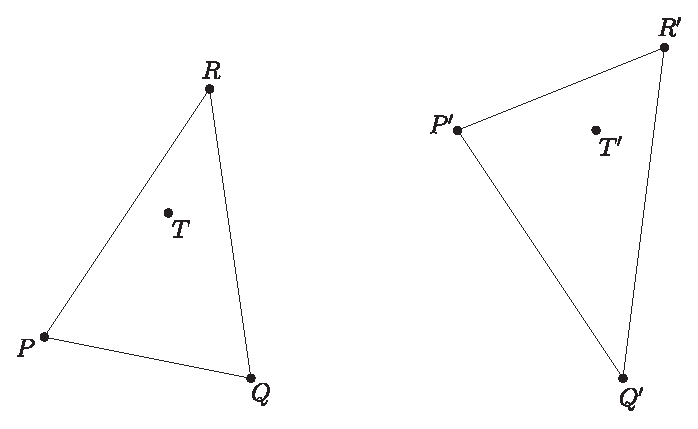
\includegraphics{skript/grafiken/lineare-algebra-2-9-3-a}
\end{center}

\paragraph{Beobachtung:} Seien $\vec{p}, \vec{q}, \vec{r} \in \real^2$ Ortsvektoren der Punkte $P$, $Q$ und $R$.
\begin{itemize}
    \item Die Punkte $P$, $Q$ und $R$ liegen genau dann auf einer Linie, wenn
    $$ \text{mydet}(\vec{p}, \vec{q}, \vec{r}) = 0 $$
    \item Der Punkt $R$ liegt genau dann links von der gerichteten Geraden $\overrightarrow{PQ}$, wenn
    $$ \text{mydet}(\vec{p}, \vec{q}, \vec{r}) > 0 $$
    \item Der Punkt $R$ liegt genau dann rechts von der gerichteten Geraden $\overrightarrow{PQ}$, wenn
    $$ \text{mydet}(\vec{p}, \vec{q}, \vec{r}) < 0 $$
    \item Die Fl�che es von $P$, $Q$ und $R$ aufgespannten Dreiecks betr�gt:
    $$ \left| \frac{\text{mydet}(\vec{p}, \vec{q}, \vec{r})}{2} \right| $$
\end{itemize} \pagebreak

\paragraph{Beispiel:} Seien $P = (-2, -3)$, $Q = (3, 5)$ und $R = (8, 14)$ Punkte in $\real^2$:
\begin{center}
    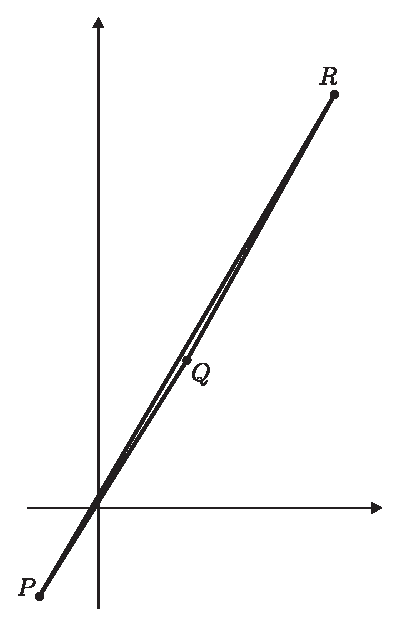
\includegraphics{skript/grafiken/lineare-algebra-2-9-3-b}
\end{center}
Bestimmung von $\text{mydet}$:
$$ \begin{vmatrix}
  -2 & 3 & 8 \\
  -3 & 5 & 14 \\
  1 & 1 & 1 \\
\end{vmatrix} = -10 + 42 - 24 - 40 + 9 + 28 = 5 > 0 $$
Daraus folgt, dass $(8, 14)$ links von der gerichteten Geraden $\overrightarrow{(-2, -3) (3, 5)}$ liegt und dass die Fl�che des von den drei Punkten aufgespannten Dreiecks $2,5$ betr�gt.

\paragraph{Beobachtung:} Diese Eigenschaften lassen sich auch auf h�here Dimensionen �bertragen. Seien $P$, $Q$, $R$ und $S$ Punkte in $\real^3$, dann ist
$$ \frac{1}{6} \cdot \begin{vmatrix}
  p_x & q_x & r_x & s_x \\
  p_y & q_y & r_y & s_y \\
  p_z & q_z & r_z & s_z \\
  1 & 1 & 1 & 1 \\
\end{vmatrix} $$
das Volumen des von den vier Punkten aufgespannten Simplexes. Falls die vier Punkte auf einer Ebene liegen, ist der Wert $0$.

\paragraph{Definition:} F�r $A \in M(n \times n, K)$ wird die \emph{komplement�re Matrix}\index{komplement�re Matrix} $\tilde{A} = (\tilde{a}_{i \, j})_{(i, j) \in n^2}$ definiert durch:
$$ \tilde{a}_{i \, j} = (-1)^{i+j} \cdot \text{det } A_{j \, i} $$
Dabei ist $A_{j \; i}$ die Matrix, die man aus $A$ durch Streichen der $j$-ten Zeile und der $i$-ten Spalte enth�lt.

\paragraph{Beobachtung:} Man kann leicht nachrechnen, dass auf der Diagonalen von $A \cdot \tilde{A}$ immer $\text{det } A$ steht, denn das is die Zeilenentwicklung von $\text{det } A$. Mit etwas mehr Aufwand kann man zeigen, dass sonst nur Nullen in $A \cdot \tilde{A}$ auftreten:
$$ A \cdot \tilde{A} = \begin{pmatrix}
  \text{det } A & 0 & \cdots & \cdots & 0 \\
  0 & \text{det } A & \ddots & \ddots & \vdots \\
  \vdots & \ddots & \ddots & \ddots & \vdots \\
  \vdots & \ddots & \ddots & \text{det } A & 0 \\
  0 & \cdots & \cdots & 0 & \text{det } A \\
\end{pmatrix} $$

\paragraph{Folgerung:} Ist $\text{det } A \neq 0$, dann ist $A$ invertierbar und
$$ A^{-1} = \frac{\tilde{A}}{\text{det } A} $$

\paragraph{Spezialfall:} F�r $A \in M(2 \times 2, K)$ gilt:
$$ \begin{pmatrix}
  a & b \\
  c & d \\
\end{pmatrix}^{-1} = \frac{1}{ad - bc} \cdot \begin{pmatrix}
  d & -b \\
  -c & a \\
\end{pmatrix} \platz \text{f�r} \platz ad - bc \neq 0 $$

\paragraph{Satz:} F�r alle $A, B \in M(n \times n, K)$ gilt:
$$ \text{det}(A \cdot B) = \text{det } A \cdot \text{det } B $$

\paragraph{Folgerung:} Man kann jeden Endomorphismus $f : K^n \rightarrow K^n$ eindeutig seine Determinante zuordnen als $\text{det } A$ f�r diese Matrix $A$ von $f$ bez�glich der Standardbasis.

\paragraph{Satz:} Sei $f : K^n \rightarrow K^n$ ein Endomorphismus, $A$ die zu $f$ geh�rende Matrix bez�glich der Standardbasis und $B$ eine zu $f$ geh�rende Matrix bez�glich einer anderen Basis, dann gilt:
$$ \text{det } A = \text{det } B $$

%%%%%%%%%%%%%%%%%%%%%%%%%%%%%%%%%%%%%%%%%%%%%%%%%%%%%%%%%%%%%%%%%%%%%%%%%%%%%%%
%%%%%%%%%%%%%%%%%%%%%%%%%%%%%%%%%%%%%%%%%%%%%%%%%%%%%%%%%%%%%%%%%%%%%%%%%%%%%%%
%%%%%%%%%%%%%%%%%%%%%%%%%%%%%%%%%%%%%%%%%%%%%%%%%%%%%%%%%%%%%%%%%%%%%%%%%%%%%%%
% Hier fortfahren
%%%%%%%%%%%%%%%%%%%%%%%%%%%%%%%%%%%%%%%%%%%%%%%%%%%%%%%%%%%%%%%%%%%%%%%%%%%%%%%
%%%%%%%%%%%%%%%%%%%%%%%%%%%%%%%%%%%%%%%%%%%%%%%%%%%%%%%%%%%%%%%%%%%%%%%%%%%%%%%
%%%%%%%%%%%%%%%%%%%%%%%%%%%%%%%%%%%%%%%%%%%%%%%%%%%%%%%%%%%%%%%%%%%%%%%%%%%%%%%

\pagebreak

\begin{center}
    ... Vorlesung vom 19.12.2002 (fehlt)
\end{center} \pagebreak

%%%%%%%%%%%%%%%%%%%%%%%%%%%%%%%%%%%%%%%%%%%%%%%%%%%%%%%%%%%%%%%%%%%%%%%%%%%%%%%
% Euklidische Vektorr�ume
%%%%%%%%%%%%%%%%%%%%%%%%%%%%%%%%%%%%%%%%%%%%%%%%%%%%%%%%%%%%%%%%%%%%%%%%%%%%%%%
\section{Euklidische Vektorr�ume}

\paragraph{Definition:} Sei $V$ ein reeller Vektorraum. Ein Skalarprodukt �ber $V$ ist eine Abbildung $< \; , \; > : V \times V \rightarrow \real$ mit folgenden drei Eigenschaften:
\begin{enumerate}
    \item Biliniarit�t, d.h. f�r jedes $\vec{v} \in V$ sind die Abbildungen
    \begin{itemize}
        \item $< \; , \vec{v} > : V \rightarrow \real$ mit $\vec{w} \mapsto <\vec{w}, \vec{v}>$ oder
        \item $< \vec{v} , \; > : V \rightarrow \real$ mit $\vec{w} \mapsto <\vec{v}, \vec{w}>$
    \end{itemize}
    sind linear.
    \item Symmetrie, d.h. $<\vec{v}, \vec{w}> = <\vec{w}, \vec{v}>$ f�r alle $\vec{v}, \vec{w} \in V$.
    \item Positive Definitheit, d.h. $<\vec{v}, \vec{v}> > 0$ f�r alle $\vec{v} \neq \vec{0}$.
\end{enumerate}
Ein Euklidischer Vekttorraum ist ein reeller Vektorraum mit einem Skalarprodukt.

\paragraph{Beispiele:}
\begin{enumerate}
    \item $V = \real^n$, Standardskalarprodukt:
    $$ \left\langle (\scalarlist{x}{n}), (\scalarlist{y}{n}) \right\rangle = x_1 y_1 \cdot x_2 y_2 + \ldots + x_n y_n $$
    $$ \left\langle (1, 5, 0, 3), (3, 0, 7, -4) \right\rangle = 3 + 0 + 0 + (-12) = -9 $$
    \item $V = \{ f : [-1, 1] \rightarrow \real \; | \; \text{stetige Funktion} \}$
    $$ \langle f, g \rangle := \int_{-1}^1 f(x) g(x) dx $$
\end{enumerate}

\paragraph{Definition:} Die Norm eines Vektors $\vec{v}$ in einem Euklidischen Raum ist definiert durch
$$ \| \vec{v} \| = \langle \vec{v}, \vec{v} \rangle $$

\paragraph{Beispiel:}
$$ \| (1, 2, 0, 2, 4) \| = \sqrt{1+4+0+4+16} = \sqrt{25} = 5 $$
Das ist auch der Abstand zwischen $(0, 0, \ldots 0)$ und $(1, 2, 0, 2, 4)$ in $\real^5$.

\paragraph{Beispiel:} in $\real^3$
$\ldots$

\paragraph{Satz (Ungleichung von Cauchy-Schwarz):} In jedem Euklidschen Vektorraum gilt f�r alle $\vec{u}, \vec{v} \in V$
$$ | \langle \vec{u}, \vec{v} \rangle | \leq \| \vec{u} \| \cdot \| \vec{v} \| $$
Speziell f�r $\real^n$ mit $\vec{u} = (\scalarlist{a}{n})$ und $\vec{v} = (\scalarlist{b}{n})$:
$$ | a_1 b_1 + a_2 b_2 + \ldots + a_n b_b | \leq \sqrt{\scalarlist{a^2}{n}} \cdot \sqrt{\scalarlist{b^2}{n}} $$
F�r $V = \{ f : [-1, 1] \rightarrow \real \; | \; \text{stetige Funktion} \}$:
$$ | \int_{-1}^1 f(x) g(x) dx | \leq \sqrt{\int_{-1}^1 (f(x))^2 dx} \cdot \sqrt{\int_{-1}^1 (g(x))^2 dx} $$

\paragraph{Beweis:}
\begin{enumerate}
    \item Fall 1: $\vec{v} = \vec{0}$, dann ergibt die Cauchy-Schwarz-Ungleichung $0 = 0$ (also korrekt)
    \item Fall 2: $\vec{v} \neq \vec{0}$
    $$ \lambda := \frac{\langle \vec{u}, \vec{v} \rangle}{\langle \vec{v}, \vec{v} \rangle} = \frac{\langle \vec{u}, \vec{v} \rangle}{\| \vec{v} \|^2} $$
    Nun betrachtet man:
    \begin{eqnarray*}
        0 &\leq& \langle \vec{u} - \lambda \vec{v}, \vec{u} - \lambda \vec{v} \rangle \\
          &=&    \langle \vec{u}, \vec{u} - \lambda \vec{v} \rangle - \lambda \langle \vec{v}, \vec{u} - \lambda \vec{v} \rangle \\
          &=&    \langle \vec{u}, \vec{u} \rangle - \lambda \langle \vec{u}, \vec{v} \rangle - \lambda \langle \vec{v}, \vec{u} \rangle + \lambda^2 \langle \vec{v}, \vec{v} \rangle \\
          &=&    \| \vec{u} \|^2 - 2 \cdot \frac{\langle \vec{u}, \vec{v} \rangle^2}{\| \vec{v} \|} + \frac{\langle \vec{u}, \vec{v} \rangle^2 \cdot \| \vec{v} \|^2}{\| \vec{v} \|^4} \\
          &=&    \| \vec{u} \|^2 - \frac{\langle \vec{u}, \vec{v} \rangle^2}{\| \vec{v} \|^2}
    \end{eqnarray*}
    Also:
    $$ \langle \vec{u}, \vec{v} \rangle^2 \leq \| \vec{u} \|^2 \cdot \| \vec{v} \|^2 \platz \Rightarrow \platz | \langle \vec{u}, \vec{v} \rangle | \leq \| \vec{u} \| \cdot \| \vec{v} \| $$
\end{enumerate}

\paragraph{Satz:} Die Norm in einem Euklidischen Vektorraum hat die folgenden Eigenschaften:
\begin{enumerate}
    \item $\| \vec{v} \| \geq 0$ f�r alle $\vec{v} \in V$
    \item $\| \vec{v} \| = 0 \platz \Leftrightarrow \platz \vec{v} = \vec{0}$
    \item $\| \lambda \vec{v} \| = | \lambda | \| \vec{v} \|$
    \item $\| \vec{v} + \vec{u} \leq \| \vec{v} \| + \| \vec{u} \| \|$
\end{enumerate}

\paragraph{Beweis:}
\begin{enumerate}
    \item
    \begin{eqnarray*}
        \| \lambda \vec{v} \| &=& \sqrt{\langle \lambda \vec{v}, \lambda \vec{v} \rangle} \\
                              &=& \sqrt{\lambda \langle \vec{v}, \lambda \vec{v} \rangle} \\
                              &=& \sqrt{\lambda^2 \langle \vec{v}, \vec{v} \rangle} \\
                              &=& \sqrt{\lambda^2} \cdot \sqrt{\langle \vec{v}, \vec{v} \rangle} \\
                              &=& |\lambda| \| \vec{v} \|
    \end{eqnarray*}
    \item
    \begin{eqnarray*}
        (\| \vec{v} \| + \| \vec{u} \|)^2 &=& \| \vec{v} \|^2 + 2 \| \vec{v} \| \| \vec{u} \| + \| \vec{u} \|^2 \\
                                          &\geq& \| \vec{v} \|^2 + 2 \langle \vec{v}, \vec{u} \rangle + \| \vec{u} \|^2 \\
                                          &=& \langle \vec{v}, \vec{v} \rangle + 2 \langle \vec{v}, \vec{u} \rangle + \langle \vec{u}, \vec{u} \rangle \\
                                          &=& \ldots
    \end{eqnarray*}
\end{enumerate}

\paragraph{Beispiel:} Normale Dreiecksungleichung aus der Geometrie:
\begin{center}
    GRAFIK
\end{center}

\paragraph{Winkel:} F�r $\vec{v}, \vec{w} \in V$ definieren wir den �ffnungswinkel
$$ \alpha (\vec{v}, \vec{w}) = \arccos \frac{\langle \vec{v}, \vec{w} \rangle}{\| \vec{v} \| \| \vec{w} \|} $$

\begin{center}
    GRAFIK mit $\vec{v} = (1, 0)$ und $\vec{w} = (2, 2)$
\end{center}
\begin{eqnarray*}
    \sphericalangle(\vec{v}, \vec{w}) &=& \arccos \left( \frac{1 \cdot 2 + 0 \cdot 2}{\sqrt{1 + 0} + \sqrt{2^2}{2^2}} \right) \\
                                      &=& \arccos \left( \frac{2}{2 \cdot \sqrt{2}} \right) \\
                                      &=& \frac{\pi}{4} = 45�
\end{eqnarray*}

In Kosinussatz die Formel einsetzen.
\begin{eqnarray*}
    c^2 &=& a^2 + b^2 - 2ab \cos \varphi \\
    c^2 = \langle \vec{u} - \vec{v}, \vec{u} - \vec{v} \rangle = \langle \vec{u}, \vec{u} \rangle + \langle \vec{v}, \vec{v} \rangle - 2 \langle \vec{u}, \vec{v} \rangle \\
    &=& \| \vec{u} \|^2 + \| \vec{v} \|^2 - 2 \| \vec{u} \| \| \vec{v} \| \cdot \frac{\langle \vec{u}, \vec{v} \rangle}{\| \vec{u} \| \| \vec{v} \|} \\
    &=& a^2 + b^2 - 2ab \cos \varphi \\
    \varphi &=& \arccos \frac{\langle \vec{u}, \vec{v} \rangle}{\| \vec{u} \| \| \vec{v} \|}
\end{eqnarray*}

\begin{center}
    GRAFIK: Kosinus- ($0 \rightarrow \pi$) und Arcuskosinus-Funktion
\end{center}

\paragraph{Definition:} Zwei Vektoren $\vec{u}$ und $\vec{v}$ in einem Euklidischen Vektorraum $(V, \langle \; , \; \rangle)$ hei�en orthogonal (senkrecht) zueinander, wenn $\langle \vec{u}, \vec{v} \rangle = 0$ ist.
$$ \sphericalangle (\vec{u}, \vec{v}) = \frac{\pi}{2} \platz \Leftrightarrow \platz  \langle \vec{u}, \vec{v} \rangle = 0 \platz \Leftrightarrow \platz \text{$\vec{u}$ steht senkrecht auf $\vec{v}$} $$
Schreibweise:
$$ \vec{u} \bot \vec{v} $$
F�r eine Teilmenge $M \subseteq V$ schreibt man $M \bot \vec{u}$, falls $\langle \vec{v}, \vec{u} \rangle = 0$ f�r alle $\vec{v} \in M$.

\paragraph{Definition:} Das orthogonale Komplement $M^{\bot}$ einer Menge $M \subseteq V$ ist definiert als
$$ M^{\bot} = \{ \vec{u} \in V \; | \; M \bot \vec{u} \} $$
\begin{center}
    GRAFIK: einige Vektoren aus $M$ (auf einer Linie) und einige aus $M^{\bot}$ (auch auf einer Linie, aber orthogonal zu den aus $M$)
\end{center}

\paragraph{Satz:} Die Menge $M^{\bot}$ ist ein Unterraum.

\paragraph{Beweis:}
\begin{itemize}
    \item Der Nullvektoren geh�rt zu $M^{\bot}$.
    \item Addition:
    \begin{eqnarray*}
        \vec{u}, \vec{u'} \in M^{\bot} &\Rightarrow& \langle \vec{u}, \vec{v} \rangle = \langle \vec{u'}, \vec{v} \rangle = 0 \platz \text{f�r alle $\vec{v} \in M$} \\
        &=& \langle \vec{u} + \vec{u'}, \vec{v} \rangle = \langle \vec{u}, \vec{v} \rangle + \langle \vec{u'}, \vec{v} \rangle = 0 \\
        &\Rightarrow& \vec{u} + \vec{u'} \in M^{\bot}
    \end{eqnarray*}
    \item Multiplikation: $\ldots$
\end{itemize}

\paragraph{Definition:} Eine Menge von Vektoren $\veclist{v}{r}$ wird Orthonormalsystem genannt, falls $\| \vec{v}_i \| = 1$ f�r alle $i = 1, 2, \ldots r$ und $\langle \vec{v}_i, \vec{v}_j \rangle = 0$ f�r alle $i \neq j$. \par
k�rzer:
$$ \langle \vec{v}_i, \vec{v}_j \rangle = \delta_{i \, j} = \left\{ \begin{array}{lll} 1 &\text{ falls }& i = j \\ 0 &\text{sonst}& \end{array} \right.$$

\paragraph{Beispiel:} Standardbasis f�r 4D.

\paragraph{Lemma 1:} Die Vektoren eines Orthogonalsystem sind linear unabh�ngig.

\paragraph{Beweis:} Angenommen $\veclk{v}{\lambda}{r} = \vec{0}$. \par
Zeige: $\lambda_1 = \lambda_2 = \ldots = \lambda_r = 0$ \par
\begin{eqnarray*}
    0 &=& \langle \vec{0}, \vec{v}_i \rangle \\
      &=& \langle \veclk{v}{\lambda}{r}, \vec{v}_i \rangle \\
      &=& \underbrace{\lambda_1 \langle \vec{v}_1, \vec{v}_i \rangle}_{=0} + \ldots + \underbrace{\lambda_i \langle \vec{v}_i, \vec{v}_i \rangle}_{=1} + \ldots + \underbrace{\lambda_r \langle \vec{v}_r, \vec{v}_i \rangle}_{=0} \\
      &=& \lambda_i
\end{eqnarray*}

\paragraph{Lemma 2:} Ist $\{ \veclist{v}{n} \ \}$ eine orthonormale Basis von $V$, so gilt f�r jedes $\vec{v} \in V$ die folgende Entwicklungsformel:
$$ \vec{v} = \sum_{i=1}^n \langle \vec{v}, \vec{v}_i \rangle \vec{v}_i $$

\paragraph{Beweis:} Nachrechnen

\paragraph{Beispiel:} $\vecthree{1}{0}{0}$, $\vecthree{0}{1}{0}$, $\vecthree{0}{0}{1}$
$$ \vecthree{2}{3}{0} = (2+0+0) \vecthree{1}{0}{0} + (0+3+0) \vecthree{0}{1}{0} + (0+0+0) \vecthree{0}{0}{1} $$

\paragraph{Lemma 3:} Ist $\veclist{v}{r}$ ein Orthonormalsystem in $V$ und $U = \text{Lin}(\{ \veclist{v}{r} \})$, so hat jedes $\vec{v} \in V$ eine eindeutige Darstellung
$$ \vec{v} = \vec{u} + \vec{w} \text{ mit } \vec{u} \in U \text{ und } \vec{w} \in U^{\bot} $$
Dabei ist
$$ \vec{u} = \sum_{i=0}^r \langle \vec{v}, \vec{v}_i \rangle \vec{v}_i $$
und
$$ \vec{w} = \vec{v} - \vec{u} $$

\paragraph{Beispiel:} $V = \real^2$, $r = 1$, $\vec{v}_1 = \vectwo{\frac{\sqrt{2}}{2}}{\frac{\sqrt{2}}{2}}$, $\| \vec{v}_1 \| = 1$ \par
$\vec{v} = \vectwo{3}{2} = \vec{u} + \vec{w}$ wobei $\vec{u} \in \text{Lin}(\vec{v}_1)$ und $\vec{w} \bot \vec{v}_1$
\begin{center}
    GRAFIK: $U$ mit $\vec{v}_1$ und $U^{\bot}$, au�erdem $\vec{v}$, $\vec{v}$ wird auf $U$ und $U^{\bot}$ projiziert
\end{center}
\begin{eqnarray*}
    \vec{u} &=& \langle \vec{v}, \vec{v}_1 \rangle \vec{v}_1 \\
            &=& \frac{5 \sqrt{2}}{2} \vectwo{\frac{\sqrt{2}}{2}}{\frac{\sqrt{2}}{2}} \\
            &=& \vectwo{\frac{5}{2}}{\frac{5}{2}} \\
    \vec{w} &=& \vectwo{3}{2} - \vectwo{\frac{5}{2}}{\frac{5}{2}} = \vectwo{\frac{1}{2}}{-\frac{1}{2}}
\end{eqnarray*}

\paragraph{Satz (Erhard Schmidt'sches Orthonormalisierungsverfahren):} Sei $\{ \veclist{v}{r} \}$ linear unabh�ngig, dann bilden die Vektoren
\begin{eqnarray*}
    \tilde{v}_1 &=& \frac{\vec{v}_1}{\| \vec{v}_1 \|} \\
    \tilde{v}_{k+1} &=& \frac{\vec{v}_{k+1} - \sum_{i=1}^k \langle \vec{v}_{k+1}, \tilde{v}_i \rangle \tilde{v}_i}{\left\| \vec{v}_{k+1} - \sum_{i=1}^k \langle \vec{v}_{k+1}, \tilde{v}_i \rangle \tilde{v}_i \right\|} \platz \text{f�r $k = 1, 2, \ldots r-1$}
\end{eqnarray*}
ein Orthonormalsystem mit den Eigenschaften, dass
$$ \text{Lin}(\{ \vec{v}_1, \vec{v}_2, \ldots \vec{v}_i \}) = \text{Lin}(\{ \tilde{v}_1, \tilde{v}_2, \ldots \tilde{v}_i \}) $$
f�r $i = 1, 2, \ldots r$.

\paragraph{Beispiel:} $\vec{v}_1 = \vecthree{2}{2}{0}$, $\vec{v}_2 = \vecthree{-3}{-1}{0}$, $\vec{v}_3 = \vecthree{1}{2}{3}$
\begin{eqnarray*}
    \tilde{v}_1 &=& \frac{1}{\sqrt{8}} \vecthree{2}{2}{0} = \vecthree{\frac{\sqrt{2}}{2}}{\frac{\sqrt{2}}{2}}{0} \\
    \tilde{v}_2 - \langle \vec{v}_2, \tilde{v}_1 \rangle \tilde{v}_1 &=& \vecthree{-3}{-1}{0} - (-2 \sqrt{2}) \vecthree{\frac{\sqrt{2}}{2}}{\frac{\sqrt{2}}{2}}{0} \\
    &=& \vecthree{-3}{-1}{0} + \vecthree{2}{2}{0} \\
    &=& \vecthree{-1}{1}{0} \\
    \tilde{v}_2 &=& \frac{\vecthree{-1}{1}{0}}{\left\| \vecthree{-1}{1}{0} \right\|} \\
    &=& \vecthree{\frac{-\sqrt{2}}{2}}{\frac{\sqrt{2}}{2}}{0} \\
    \vecthree{1}{2}{3} - \frac{3\sqrt{2}}{2} \tilde{v}_1 - \frac{\sqrt{2}}{2} \tilde{v}_2 \\
    &=& \vecthree{1}{2}{3} - \vecthree{\frac{3}{2}}{\frac{3}{2}}{0} - \vecthree{-\frac{1}{2}}{\frac{1}{2}}{0} \\
    &=& \vecthree{.}{.}{.} \\
    \tilde{v}_3 &=& \ldots \text{Normieren}
\end{eqnarray*}

\paragraph{Definition:} Orthogonale Projektion von $\vec{v}$ in den Unterraum $U = \text{Lin}(\veclist{v}{r})$
$$ P_U(\vec{v}) = \langle \vec{v}, \vec{v}_1 \rangle \cdot \vec{v}_1 + \ldots + \langle \vec{v}, \vec{v}_r \rangle \cdot \vec{v}_r \in U $$
$\vec{w} := \vec{v} - P_U(\vec{v})$ , man kann zeigen, dass $\vec{w} \bot U$, d.h. $\vec{w} \in U^{\bot}$, folglich ist $P_U(\vec{w}) = \vec{0}$

\begin{center}
    GRAFIK
\end{center}

Die Orthonormalprojektion $P_U :  V \rightarrow U$ hat die folgenden zwei Eigenschaften:
\begin{itemize}
    \item $P_U$ beschr�nkt auf $U$ ist die identische Abbildung
\end{itemize}

\paragraph{Beispiel:} $U = \text{Lin}\left( \vectwo{2}{1} \right)$ in $V = \real^2$ \par
Aufgabe: Berechne die Matrix der Projektion $P_U$.
\begin{center}
    GRAFIK: Gerade $y = \frac{1}{2}x$ mit Projektion der Basisvektoren $\vectwo{1}{0}$ und $\vectwo{0}{1}$ auf die Gerade
\end{center}
\begin{enumerate}
    \item Orthonormalbasis f�r $U$
    \begin{eqnarray*}
        \vec{v}_1 &=& \vectwo{2}{1} \\
        \tilde{v}_1 &=& \frac{\vectwo{2}{1}}{\left\| \vectwo{2}{1} \right\|} = \frac{\vectwo{2}{1}}{\sqrt{5}} = \vectwo{\frac{2}{\sqrt{5}}}{\frac{1}{\sqrt{5}}}
    \end{eqnarray*}
    \item Projektion
    $$ P_U(\vec{v}) = \langle \vec{v}, \tilde{v}_1 \rangle \cdot \tilde{v}_1 $$
    Setze f�r $\vec{v}$ die Basisvektoren $\vec{e}_1$ und $\vec{e}_2$ ein:
    \begin{eqnarray*}
        P_U \left( \vectwo{1}{0} \right) &=& \left\langle \vectwo{1}{0}, \vectwo{\frac{2}{\sqrt{5}}}{\frac{1}{\sqrt{5}}} \right\rangle \cdot \vectwo{\frac{2}{\sqrt{5}}}{\frac{1}{\sqrt{5}}} = \vectwo{\frac{4}{5}}{\frac{2}{5}} \\
        P_U \left( \vectwo{0}{1} \right) &=& \left\langle \vectwo{0}{1}, \vectwo{\frac{2}{\sqrt{5}}}{\frac{1}{\sqrt{5}}} \right\rangle \cdot \vectwo{\frac{2}{\sqrt{5}}}{\frac{1}{\sqrt{5}}} = \vectwo{\frac{2}{5}}{\frac{1}{5}}
    \end{eqnarray*}
    \item Matrix:
    $$ \begin{pmatrix}
      \frac{4}{5} & \frac{2}{5} \\
      \frac{2}{5} & \frac{1}{5} \\
    \end{pmatrix} =
    \begin{pmatrix}
      0,8 & 0,4 \\
      0,4 & 0,2 \\
    \end{pmatrix} $$
\end{enumerate}

%%%%%%%%%%%%%%%%%%%%%%%%%%%%%%%%%%%%%%%%%%%%%%%%%%%%%%%%%%%%%%%%%%%%%%%%%%%%%%%
% Affiner Raum (intuitiver Zugang)
%%%%%%%%%%%%%%%%%%%%%%%%%%%%%%%%%%%%%%%%%%%%%%%%%%%%%%%%%%%%%%%%%%%%%%%%%%%%%%%
\section{Affiner Raum (intuitiver Zugang)}

\paragraph{Motivation:} Anwendung des Skalarprodukts in der affinen Geometrie

\paragraph{Mengen:}
\begin{itemize}
    \item $V$ Vektorraum (hier �ber $\real$, d.h. $V = \real^2, \real^3$)
    \item $A$ Punktmenge
\end{itemize}

\paragraph{Operationen:}
\begin{itemize}
    \item $\text{Punkt} + \text{Vektor} \mapsto \text{Punkt}$
    \item $\text{Punkt} - \text{Punkt} \mapsto \text{Vektor}$
\end{itemize}
\begin{center}
    GRAFIK: zwei Punkte $p$ und $q$ und ein Verbindungsvektor $\vec{v}$ mit
    \begin{eqnarray*}
        \vec{q} &=& p + \vec{v} \\
        \vec{v} &=& q - p
    \end{eqnarray*}
    Eigenschaft:
    \begin{eqnarray*}
        p + (\vec{v} + \vec{w}) &=& (p + \vec{v}) + \vec{w}
    \end{eqnarray*}
\end{center}
Standardmodell f�r $A$ ist $V$ selbst.

\paragraph{affiner Unterraum:} $U \subseteq V$ Untervektorraum, $p \in A$
$$ p + U = \{ p + \vec{u} \; | \; \vec{u} \in U \} $$

\paragraph{Beispiele:}
\begin{itemize}
    \item affine Unterr�ume in $A = \real^2$:
    \begin{itemize}
        \item Punkte ($\text{dim } U = 0$)
        \item Geraden ($\text{dim } U = 1$)
        \item ganz $\real^2$ ($\text{dim } U = 2$)
    \end{itemize}
    \item affine Unterr�ume in $A = \real^3$:
    \begin{itemize}
        \item Punkte ($\text{dim } U = 0$)
        \item Geraden ($\text{dim } U = 1$)
        \item Ebenen ($\text{dim } U = 2$)
        \item ganz $\real^3$ ($\text{dim } U = 3$)
    \end{itemize}
\end{itemize}

\paragraph{Geradengleichungen:}
$V = A = \real^2$
\begin{enumerate}
    \item Gerade durch einen Punkt und parallel zu einem Vektorunterraum
    \begin{itemize}
        \item $U \subseteq V$ ist ein 1-dimensionaler Vektorunterraum $U = \{ \lambda \vec{u} \; | \; \lambda \in \real \}$
        \item $p \in A$
    \end{itemize}
    Gerade durch $p$ parallel zu $U$ in Parameterdarstellung:
    $$ L = \{ p + \lambda \vec{u} \; | \; \lambda \in \real \} $$
    \item Gerade durch zweu Punkte:
    \begin{itemize}
        \item $p = (x, y)$
        \item $p' = (x', y')$
    \end{itemize}
    Schreibweisen:
    \begin{eqnarray*}
        L &=& \{ p + \lambda (p' - p) \; | \; \lambda \in \real \} \\
          &=& \{ q = (x_q, y_q) \; | \; x_q = x + \lambda(x' - x), y_q = y + \lambda(y' - y), \lambda \in \real \} \\
          &=& \{ q = (x_q, y_q) \; | \; \underbrace{x_q (y' - y) - x(y' - y)}_{= \lambda (x' - x) (y' - y)} = \underbrace{y_q (x' - x) - y (x' - x)}_{= \lambda (x' - x) (y' - y)} \} \\
          &=& \{ q = (x_q, y_q) \; | \; a x_q + b y_q = c \} \hspace{1cm} \text{(Koordinantendarstellung von $L$)}
    \end{eqnarray*}
    mit $a = y' - y$, $b = x' - x$ und $c = -y (x' - x) + x (y' - y)$
\end{enumerate}

\paragraph{HNS:}
\begin{center}
    GRAFIK: Gerade $L$ und parallele Gerade $U_L$ durch den Ursprung und Normalenvektor $\vec{n}$, au�erdem $P_{U_L}(q - 0)$ und $\vec{w} = d \cdot \vec{n}$
\end{center}

\begin{itemize}
    \item Normalenvektor $\vec{n}$ von $L$ ist senkrecht zu $U_L$ und $\| \vec{n} \| = 1$
    \item Abstand $d$ von $(0, 0)$ zu $L$, d.h. $(0, 0) + d \cdot \vec{n} \in L$
\end{itemize}

Hesse-Normalform von $L$:
$$ L = \{ q \; | \; \langle q - 0, \vec{n} \rangle = d \} $$

Das hei�t:
\begin{eqnarray*}
    \langle q - 0, \vec{n} \rangle &=& \langle P_{U_L}(q - 0), \vec{n} \rangle + \langle \vec{w}, \vec{n} \rangle \\
                                   &=& 0 + \langle d \vec{n}, \vec{n} \rangle \\
                                   &=& d \langle \vec{n}, \vec{n} \rangle \\
                                   &=& d
\end{eqnarray*}

Bestimmung der Hesse-Normalform aus der Parameterform:
$$ L = \{ p + \lambda \vec{v} \; | \; \lambda \in \real \} $$
Aufgabe: Bestimme $\vec{n}$ und $d$!
\begin{enumerate}
    \item $\tilde{v} = \frac{\vec{v}}{\| \vec{v} \|}$ Orthonormalbasis von $U_L$
    \item $\vec{n}' = d \vec{n} = (p-0) - P_{U_L}(p-0) = (p-0) - \langle (p-0), \tilde{v} \rangle \cdot \tilde{v}$
    \item $d = \| \vec{n}' \|$ und $\vec{n} = \frac{\vec{n}'}{d}$
\end{enumerate} \pagebreak

\begin{center}
   ... Vorlesung vom 16.02.2002 (fehlt)
\end{center} \pagebreak

\begin{center}
   ... Vorlesung vom 21.02.2002 (fehlt)
\end{center} \pagebreak

\chapter{Endliche K�rper und Codierungstheorie}

%%%%%%%%%%%%%%%%%%%%%%%%%%%%%%%%%%%%%%%%%%%%%%%%%%%%%%%%%%%%%%%%%%%%%%%%%%%%%%%
% Restklassenarithmetik
%%%%%%%%%%%%%%%%%%%%%%%%%%%%%%%%%%%%%%%%%%%%%%%%%%%%%%%%%%%%%%%%%%%%%%%%%%%%%%%
\section{Restklassenarithmetik}
%%%%%%%%%%%%%%%%%%%%%%%%%%%%%%%%%%%%%%%%%%%%%%%%%%%%%%%%%%%%%%%%%%%%%%%%%%%%%%%
\subsection{...}

\begin{center}
   ... Vorlesung vom 21.02.2002 (fehlt)
\end{center} \pagebreak

\begin{eqnarray*}
    252 &=& 1 \cdot 138 + 54 \\
    158 &=& 3 \cdot 53 + 36 \\
    54 &=& 1 \cdot 36 + 18 \\
    36 &=& 2 \cdot 18 + 0
\end{eqnarray*}

Die Umkehrung des Euklidischen Algorithmus  liefert eine Darstellung des $\text{ggT}(a, b)$ als Linearkombination aus $a$ und $b$ mit ganzzahligen Koeffizienten.

\begin{eqnarray*}
    18 &=& 54 - 1 \cdot 36 \platz (36 = 198 - 3 \cdot 54) \\
       &=& 54 - (198 - 3 \cdot 54) \\
       &=& 4 \cdot 54 - 198 \platz (54 = 252 - 198) \\
       &=& 4 \cdot (252 - 198) - 198 \\
       &=& 4 \cdot 252 - 5 \cdot 198
\end{eqnarray*}

\paragraph{Satz:} Sind $a, b \in \ganz^+$, dann existieren $r, s \in \ganz$, so dass $\text{ggT}(a, b) = r \cdot a + s \cdot b$.

\paragraph{Satz:} Seien $m$ und $a$ zwei positive, teilerfremnde Zahlen, dasnn gibt es genau ein $b \in \{ 1, 2, \ldots m-1 \}$, so dass $a \cdot b \equiv 1 (\text{mod} m)$.

\paragraph{Beweis:} $\text{ggT}(a, m) = 1 = r \cdot a + s \cdot m$ f�r geeignete $r, s \in \ganz$. Setzen $b := r \mod m \in \{ \not 0, 1, \ldots m-1 \}$.
\begin{itemize}
    \item $b \equiv r (\text{mod} m)$
    \item $a \equiv a (\text{mod} m)$
    \item $0 \equiv s \cdot m (\text{mod} m)$
    \item %\hline
    \item $a \cdot b \equiv r \cdot a (\text{mod} m)$
    \item $a \cdot b + 0 \equiv r \cdot a + s \cdot m (\text{mod} m) \equiv 1 (\text{mod} m)$
\end{itemize}
Eindeutigkeit: Angenommen $a \cdot b \equiv a \cdot c \equiv 1 (\text{mod} m)$ und $0 < c \leq b \leq m - 1$
$$ a \cdot (b-c) \equiv \underbrace{1-1}_{=0} (\text{mod} m) $$
$a \cdot (b-c)$ ist durch $m$ teilbar $\Rightarrow$ $(b-c)$ is durch $m$ teilbar und $0 \leq b-c < m-1$ $\Rightarrow$ $b-c = 0$ $\Rightarrow$ $b=c$ $\Rightarrow$ Eindeutigkeit

\paragraph{Folgerung:} Ist $p$ eine Primzahl und $a \in \{ 1, 2, \ldots p-1 \}$, dann gibt es ein eindeutiges $b \in \{ 1, 2, \ldots p-1 \}$, so dass $a \cdot b \equiv 1 (\text{mod} p)$. $b$ wird die zu $a$ inverse Zahl bez�glich $p$ genannt.

\paragraph{Folgerung:} Die Zahlen $\{ 0, 1, \ldots p-1 \}$, wobei $p$ Primzahl, bilden mit der Addition und Multiplikation modulo $p$ einen K�rper. Dieser K�rper wird mit $\ganz_p$ oder mit $\text{GF}(p)$ bezeichnet.

\paragraph{Beispiel:} $\ganz_7 = \{ 0, 1, 2, 3, 4, 5, 6 \}$:
\begin{eqnarray*}
    4 + 5 &=& 2 \\
    4 \cdot 4 &=& 2 \\ \\
    1 \cdot 1 &=& 1 \\
    6 \cdot 6 &=& 1 \\
    2 \cdot 8 &=& 1 \\
    3 \cdot 5 &=& 1 \\ \\
    3 \cdot x &=& 4 \platz | \cdot 3^{-1} \\
    \underbrace{5 \cdot 3}_{=1} \cdot x &=& 5 \cdot 4 = 6
\end{eqnarray*}

\paragraph{Beispiel:} L�se $7 \cdot x = 5$ in $\ganz_{17}$. \par
Inverses zu $7 \mod 17$:
\begin{eqnarray*}
    17 &=& 2 \cdot 7 + 3 \\
    3 &=& 17 - 2 \cdot 7 \\
    7 &=& 2 \cdot 3 + 1 \\
    1 &=& 7 - 2 \cdot 3 = 7 - 2 \cdot (17 - 2 \cdot 7) = \textbf{5} \cdot 7 - 2 \cdot 17 \\
    7^{-1} &=& (5 \mod 17) = 5 \\ \\
    7 \cdot x &=& 5 \platz | \cdot 5 \\
    1 \cdot x &=& 5 \cdot 5 = 8
\end{eqnarray*}

\paragraph{Chinesischer Restklassensatz:} Seien $m_1, m_2, \ldots m_n \in \ganz^+$ paarweise teilerfremd und $m = m_1 \cdot m_2 \cdot m_n$, dann gibt es f�r beliebige $a_1, a_2, \ldots a_n \in \ganz$ eine Zahl $x \in \{ 0, 1, \ldots m-1 \}$, so dass die folgenden Komvergenzen erf�llt sind:
\begin{eqnarray*}
    x &\equiv& a_1 (\text{mod} m_1) \\
    x &\equiv& a_2 (\text{mod} m_2) \\
      &\vdots& \\
    x &\equiv& a_n (\text{mod} m_n)
\end{eqnarray*}

\paragraph{Beispiel:} $m_1 = 99$, $m_2 = 100$, $m_3 = 101$, $a_1 = 80$, $a_2 = 63$, $a_3 = 27$

\paragraph{Beweis:}
\begin{enumerate}
    \item Finde Zahlen, die $\equiv 1 (\text{mod} m_i)$ und $\equiv 0 (\text{mod} m_j)$ mit $j \neq i$ sind
    \begin{eqnarray*}
        M_1 &=& \frac{m}{m_1} = m_2 \cdot m_3 \cdot \ldots \cdot m_n \\
        M_2 &=& \frac{m}{m_2} = \ldots \\
            &\vdots& \\
        M_n &=& \frac{m}{m_n} = \ldots \\
        \text{ggT}(m_k, M_k) = 1 \platz \text{d.h. } \exists y_k \equiv 1 (\text{mod} m_k)
    \end{eqnarray*}
    $$ M_k \cdot y_k \equiv 1 \modulo{m_k} $$
    Das sind diese Zahlen, denn $M_k \cdot y_k$ is duch jedes $m_l$ ($l \neq k$) teilbar, d.h. $M_k \cdot y_k \equiv 0 (\text{mod} m_l)$. \par
    Setze
    $$ x = (a_1 \cdot y_1 \cdot M_1 + \ldots + a_n \cdot y_n \cdot M_n) \mod m $$
    Pr�fe, dass alle Kongruenzen erf�llt sind.

\end{enumerate}

\paragraph{Kleiner Satz von Fermat:} Ist $p$ eine Primzahl, dann gilt f�r jede nicht durch $p$ teilbare Zahl $a \in \ganz$:
$$ a^{p-1} \equiv 1 \modulo{p} $$

\paragraph{Beispiele:}
\begin{itemize}
    \item W�hle $p = 7$ und $a = 2$:
    \begin{eqnarray*}
        a^6 &=& 64 \\
        64 &\equiv& 1 \modulo{7}
    \end{eqnarray*}
    \item W�hle $p = 7$ und $a = 3$:
    \begin{eqnarray*}
        a^6 &=& 729 \\
        729 &\equiv& 1 \modulo{7}
    \end{eqnarray*}
\end{itemize}

%%%%%%%%%%%%%%%%%%%%%%%%%%%%%%%%%%%%%%%%%%%%%%%%%%%%%%%%%%%%%%%%%%%%%%%%%%%%%%%
\subsection{RSA-Kryptosysteme}
Teilnehmen (party) verschicken Nachrichten $m \in \{ 0, 1 \}^n$:
\begin{center} \begin{tabular}{ccc}
Alice & & Bob \\
$m$ & & $D(E(m)) = m$ \\
$\downarrow$ & & $\downarrow$ \\
$E(m) \in \{ 0,1 \}^{l(n)}$ & $\rightsquigarrow$ & $E(m)$ \\
& $\downarrow$ & \\
Gegener (adversary) Eve & $E(m)$ & \\
& $\downarrow$ & ? \\
& $m$ &
\end{tabular} \end{center}

Rivers, Shamir, Adlerman 78
\begin{itemize}
    \item $p$, $q$ zwei gro�e Primzahlen
    \item $n = p \cdot q$
    \item $e \in \ganz$: $\text{ggT}(e, (p-1)(q-1)) = 1$
    \item $d \in \ganz$: $d \cdot e \equiv 1 \modulo{(p-1)(q-1)}$
\end{itemize}

\begin{enumerate}
    \item Bob gibt $n, e$ bekannt ($p, q, d$ geheim)
    \item Alice verschl�sselt Nachricht $m$ ($|m| < \log n$):
    $$ m' = E(m) := m^e \mod n $$
    \item Bob entschl�sselt $m'$:
    $$ D(m') := m'^d \mod n $$
\end{enumerate}
Behauptung:
$$ D(E(m)) = m $$

\paragraph{Beweis:}
$$ d \cdot e = 1 + k \cdot (p-1)(q-1) $$
Zu zeigen:
$$ (m^e)^d = m^{1 + k(p-1)(q-1)} \equiv m \modulo{n} $$
gen�gt zu zeigen (Chinesicher Restsatz):
\begin{eqnarray*}
    (m^e)^d &\equiv& m \modulo{p} \\
    \text{und} \platz (m^e)^d &\equiv& m \modulo{q}
\end{eqnarray*}
\begin{enumerate}
    \item Fall 1:
    \begin{eqnarray*}
        m &\equiv& 0 \modulo{p}
    \end{eqnarray*}
    (trivial)
    \item Fall 2:
    \begin{eqnarray*}
        (m^e)^d &\equiv& m \cdot (m^{p-1})^{(q-1) \cdot k} \\
                &\equiv& m \cdot 1^{(p-1) \cdot k} \modulo{p} \\ \\
        (m^d)^d &\equiv& m \modulo{p}
    \end{eqnarray*}
\end{enumerate}

Authetisierung mit RSA:
\begin{itemize}
    \item 2'): Alice schickt Zufallsstring $m$
    \item 3'): Bob schickt $m' = D(m)$ zur�ck
    \item 4'): Alice �berpr�ft $E(m') = m$ ?
\end{itemize}

Vorteile:
\begin{itemize}
    \item Parameter leicht zu erzeugen (randomisierter Primzahltest)
    \item Ver- und Entschl�sselung leicht zu berechnen (Spezialchip)
    \item sicher in der Praxis (unter Einhaltung bestimmter Regeln)
\end{itemize}

Nachteile:
\begin{itemize}
    \item nur sicher, wenn es \emph{keine} effiziente Algorithmen zur Faktorisierung gibt
    \item m�glicherweise auch ohne Faktorisierungsalgorithmus zu brechen
    \item mit \emph{Quantencomputern} ist Faktorisierung in Polynomialzeit m�glich (P. Shor)
\end{itemize}

Aufgabe: Kryptographie auf Grundlage $NP$-schwerer Probleme.

%%%%%%%%%%%%%%%%%%%%%%%%%%%%%%%%%%%%%%%%%%%%%%%%%%%%%%%%%%%%%%%%%%%%%%%%%%%%%%%
% Grundbegriffe der Codierungstheorie
%%%%%%%%%%%%%%%%%%%%%%%%%%%%%%%%%%%%%%%%%%%%%%%%%%%%%%%%%%%%%%%%%%%%%%%%%%%%%%%
\section{Grundbegriffe der Codierungstheorie}\label{grundcode}

Corierungstheorie -- Verschl�sselung von Informationen unter den folgenden Aspekten:
\begin{enumerate}
    \item Codierung soll helfen, eine Information geheim zu halten.
    \item Codierung soll so kurz wie m�glich sein
    \item Fehler in der �bertragung sollten erkanntund korrigiert werden.
\end{enumerate}
$\rightsquigarrow$ Teilgebiete:
\begin{enumerate}
    \item Kryptographie (RSA, Einwegfunktionen, Pseudozufallsgeneratoren, ...)
    \item Datenkompression (Hufman, ...)
    \item Fehlerkorrigierende Codes (Hamming Code, linearer Code, ...)
\end{enumerate}

\paragraph{Modell:}
\begin{center} \begin{tabular}{rcccl}
& Reininformation & & Reininformation &\\
Quellencodierung & $\downarrow$ & & $\uparrow$ & Quellencodierung \\
& Verschl�sselte Information & & Verschl�sselte Information & \\
Kanalcodierung & $\downarrow$ & & $\uparrow$ & Kanalcodierung (Fehler korrigieren) \\
& Sender & $\rightsquigarrow$ & Empf�nger & \\
& & Kanal & & \\
& & $\Uparrow$ & & \\
& & St�rung & &
\end{tabular} \end{center}
Kanalalphanet: $Q$, $|Q| = q$, h�ufig $Q = \{ 0, 1 \}$, $q = 2$

\paragraph{Definition:} Eine (Kanal-)Codierung ist eine injektive Funktion $c : I \rightarrow Q^n$, wobei $I$ eine Informationsmenge ist (z.B. Alphabet oder bereits Menge der Codew�rter aus einer Quellcodierung). Das Bild $C = \text{Im } c$ wird ein Code genannt. \par
Hier besteht der Code nur aus W�rtern gleicher L�nge, das nennt man einen Blockcode.

\paragraph{Definition:} Seinen $v = (v_1, v_2, \ldots v_n)$ und $w = (w_1, w_2, \ldots w_n) \in Q^n$. Wir definieren den Hamming-Abstand der Worte $v$ und $w$ als Anzahl der Stellen, an denen sie sich unterscheiden:
$$ d(v, w) = |\{ i \; | \; 1 \leq i \leq n \text{ und } v_i \neq w_i \}| $$

\paragraph{Beispiel:}
$$ d((0,1,\textbf{0},\textbf{1},\textbf{0},\textbf{0},1), (0,1,\textbf{1},\textbf{0},\textbf{1},\textbf{1},1)) = 4 $$

\paragraph{Beobachtung:} Der Hamming-Abstand hat alle Eigenschaften einer Abstandsfunktion, d.h. f�r alle $u, v, w \in Q^n$ gilt:
\begin{enumerate}
    \item $d(u, v) \geq 0$ und $d(u, v) = 0 \Leftrightarrow u = v$
    \item $d(u, v) = d(v, u)$
    \item $d(u, v) + d(v, w) \geq d(u, w)$ (Dreiecksungleichung)
\end{enumerate}

\paragraph{Definition:} Die Minimalabstand eines Codes $C \subseteq Q^n$ ist
$$ d(C) := \min(\{ d(c, c') \; | \; c \neq c', c, c' \in C \}) $$

Wir verwenden $c$, $c'$, $c_1$, $c_2$ f�r Codew�rter und allgemein $u, w, v$ f�r W�rter aus $Q^n$.

\paragraph{Beispiel:}
\begin{eqnarray*}
    c : \{ a, b, c, d \} &\rightarrow& Q^3 \\
    a &\mapsto& (0, 0, 0) \\
    b &\mapsto& (0, 1, 1) \\
    c &\mapsto& (1, 0, 1) \\
    d &\mapsto& (1, 1, 0) \\
\end{eqnarray*}
$$ C = \{ (0, 0, 0), (0, 1, 1), (1, 0, 1), (1, 1, 0) \} $$
$$ d(C) = 2 $$

\paragraph{Prinzip:} Wird ein Wort $w \in Q^n$ empfangen, so sucht man ein (oder besser das) Codewort $c$ mit minimalem Abstand zu $w$. \par
Wann ist $c$ richtig? \par

Empfangen $w \in Q^n$:
\begin{enumerate}
    \item $w \notin C$, dann ist ein Fehler aufgetreten
    \item Wenn wir wissen, dass h�chstens 1 Fehler aufgetreten ist, und $c \in C$ ist das einzige Codewort mit $d(w, c) = 1$, dann ist $c$ das urspr�ngliche Codewort.
\end{enumerate}

\paragraph{Definition:} Ein Code $C$ ist $k$-fehlererkennend, wenn bei jedem empfangengenen Wort $w$, das $\leq k$ Fehler, enth�lt, erkannt wird, \emph{ob} �bertragungsfehler aufgetreten sind.

\paragraph{Definition:} Ein Code $C$ ist $k$-fehlerkorrigierend, wenn bei jedem empfangenen Wort, das $\leq k$ Fehler erh�lt, die Fehler korrigiert werden k�nnn, d.h. dass das urspr�ngliche Codewort bestimmt werden kann.

\paragraph{Definition:} F�r $v \in Q^n$ definieren wir die Kugel mit Radius $t$ um $v$ durch
$$ B_t (v) = \{ w \in Q^n \; | \; d(v, w) \leq t \} $$

\begin{center}
    GRAFIK: von Henning �bertragen
\end{center}

\paragraph{Satz:} $C$ ist $k$-fehlerkorrigierend genau dann, wenn $\forall c \neq c' \in C \; B_k(c) \cap B_k(c') = \emptyset$ genau dann, wenn $d(C) \geq 2k+1$ (Minimalabstand von $C$)

\paragraph{Beweis:}
\begin{itemize}
    \item Erste �quivalenz: bei der �ertragung von $c$ treten $\leq k$ Fehler auf, dann liegt empfangenes Wort $w \in B_k(c)$, d.h. $w$ geh�rt eindeutig zu $c$.
    \item Zweite �quivalenz:
    \begin{center}
        GRAFIK: von Henning �bertragen
    \end{center}
\end{itemize}

\paragraph{Satz:} $C$ ist $k$-fehlererkennend genau dann, wenn $\forall c \in C \; B_k(c) \cap (C \backslash \{ c \}) = \emptyset$ genau dann, wenn $d(C) \geq k+1$.

\paragraph{Beweis:} wie oben

\paragraph{Beispiele:} Einfache Konstruktion mit Parit�tsbits und Mehrfachcodierung:
$$ I = Q^m \platz \text{mit} \platz Q = \{ 0, 1 \} $$
\begin{enumerate}
    \item Parit�tsbit: $c_{\text{par}} : Q^m \rightarrow Q^{m+1}$
    $$ c_{\text{par}}(v_1, v_2, \ldots v_m) = (\underbrace{v_1, v_2, \ldots v_m, p}_{\text{gerade Anzahl von 1}}) \platz \text{mit} \platz p = v_1 + v_2 + \ldots + v_m \modulo{2} $$
    Daraus folgt: $C_{\text{par}} = \text{Im } c_{\text{par}}$ hat den Minimalabstand $2$, d.h. $C_{\text{par}}$ ist $1$-fehlererkennend.
    \item Doppelcodierung: $c_2 : Q^m \rightarrow Q^{2m}$
    $$ c_2(v_1, v_2, \ldots v_m) = (v_1, v_2, \ldots v_m, v_1, v_2, \ldots v_m) $$
    Daraus folgt: $C_2 = \text{Im } c_2$ hat den Minimalsbstand $2$, d.h. $C_2$ ist $1$-fehlererkennend.
    \item Dreifachcodierung: $c_3 : Q^m \rightarrow Q^{3m}$
    $$ c_3(v_1, v_2, \ldots v_m) = (v_1, v_2, \ldots v_m, v_1, v_2, \ldots v_m, v_1, v_2, \ldots v_m) $$
    Daraus folgt: $C_3 = \text{Im } c_3$ hat den Minimalsbstand $3$, d.h. $C_3$ ist $1$-fehlerkorrigierend.
    \item Doppelcodierung mit Parit�tsbit: $c_{2 + \text{par}} : Q^m \rightarrow Q^{2m+1}$
    $$ c_{2 + \text{par}}(v_1, v_2, \ldots v_m) = (v_1, v_2, \ldots v_m, v_1, v_2, \ldots v_m, p) \platz \text{mit} \platz p = v_1 + v_2 + \ldots v_m \modulo{2} $$
    Daraus folgt: $C_{2 + \text{par}} = \text{Im } c_{2 + \text{par}}$ hat den Minimalabstand $3$:
    \begin{itemize}
        \item Fall 1: $d(v, w) = 1 \platz (v, w \in Q^m) \Rightarrow d(c_{2 + \text{par}}(v), c_{2 + \text{par}}(w)) = \underbrace{1 + 1}_{d(v, w)} + \underbrace{1}_{p}$
        \item Fall 2: $d(v, w) \geq 2 \platz (v, w \in Q^m) \Rightarrow d(c_{2 + \text{par}}(v), c_{2 + \text{par}}(w)) \geq 2 + 2 = 4$
    \end{itemize}
    d.h. $C_{2 + \text{par}}$ ist $1$-fehlerkorrigierend.
    \item Kreuzsicherungscode $m = l^2$: $c_{\text{kr}} : Q^{m} \rightarrow Q^{m + 2l}$ \par
    Stelle Elemente von $Q^m$ in einer quadratischen Matrix dar und gib f�r jede Spalte und f�r jede Zeile das Parit�tsbit dazu:
    $$ \begin{pmatrix}
      v_1 & v_2 & \cdots & v_l \\
      v_{l+1} & v_{l+2} & \cdots & v_{2l} \\
      \vdots & \vdots & \ddots & \vdots \\
      v_{(l-1)+l+1} & v_{(l-1)+l+2} & \ldots & v_{l^2} \\
    \end{pmatrix} $$
    (Bemerkung: Um Parit�tsbits in den Zeilen und Spalten erweitern (Zeilen: $p_i$, Spalten $\bar{p}_j$)) \par
    $C_{\text{kr}} = \text{Im } c_{\text{kr}}$ hat Minimalabstand $3$, d.h. ist $1$-fehlerkorrigierend. \par
    $v, w \in Q^m$
    \begin{itemize}
        \item $d(v, w) \geq 3 \Rightarrow d(c_{\text{cr}}(v), c_{\text{cr}}(w)) \geq 3$
        \item $d(v, w) = 2$ dann liegen die zwei Unterschiede in verschiedenen Zeilen $i$ und $j$ oder in verschiedenen Spalten $k, k'$
        $$ d(\ldots) \geq 2 + \underbrace{1}_{p_i} + \underbrace{1}_{p_j} $$
        \item $d(v, w)  1$, sei Unterschied in Zeile $i$ und Spalte $j$
        $$ d(\ldots) = \underbrace{1}_{d(u, v)} + \underbrace{1}_{\bar{p}_i} + \underbrace{1}_{p_j} = 3 $$
    \end{itemize}
\end{enumerate}

\paragraph{Definition:} Die Informationsrate eines Codes $C \subseteq Q^n$ ist der Quotient
$$ \frac{\log_q |C|}{n} $$
Das beschreibt das Verh�ltnis der L�ngen des Infomationsworts und des Codeworts.

\paragraph{Beispiele:}
\begin{enumerate}
    \item F�r $C_{2 + \text{par}}$:
    $$ \frac{m}{2m+1} \lesssim \frac{1}{2} $$
    \item F�r $C_{\text{kr}}$:
    $$ \frac{m + 2 \cdot \sqrt{m} - 2 \sqrt{m}}{m + 2 \cdot \sqrt{m}} = 1 - \frac{2 \cdot \sqrt{m}}{m + 2 \cdot \sqrt{m}} \approx 1 - \frac{2}{\sqrt{m}} $$
\end{enumerate}

\paragraph{Fragen:}
\begin{enumerate}
    \item Geht es noch besser?
    \item Wie korrigiert man 2 und noch mehr Fehler?
\end{enumerate}

Idee f�r eine Verbesserung (Hamming):
$$ v = (v_1, \ldots v_4) \platz Q=\{ 0, 1 \} \platz \text{+ 3 Redundanzbits} $$
\begin{eqnarray*}
    r_1 &=& v_2 + v_3 + v_4 \modulo{2} \\
    r_2 &=& v_1 + v_3 + v_4 \modulo{2} \\
    r_3 &=& v_1 + v_2 + v_4 \modulo{2}
\end{eqnarray*}
Minimalabstand $3$ \par
Codierung durch Matrixmultiplikation �ber $\ganz_2$:
$$ c(v) = \underbrace{\begin{pmatrix}
  1 & 0 & 0 & 0 \\
  0 & 1 & 0 & 0 \\
  0 & 0 & 1 & 0 \\
  0 & 0 & 0 & 1 \\
  0 & 1 & 1 & 1 \\
  1 & 0 & 1 & 1 \\
  1 & 1 & 0 & 1 \\
\end{pmatrix}}_{\text{Generatormatrix}} \cdot \begin{pmatrix}
  v_1 \\
  v_2 \\
  v_3 \\
  v_4 \\
\end{pmatrix} = \begin{pmatrix}
  v_1 \\
  v_2 \\
  v_3 \\
  v_4 \\
  r_1 \\
  r_2 \\
  r_3 \\
\end{pmatrix} $$

Zur Decodierung mit $1$-Fehlerkorrektur verwendet man die folgede Pr�fmatrix:
$$ H = \begin{pmatrix}
  1 & 0 & 1 & 0 & 1 & 0 & 1 \\
  0 & 1 & 1 & 0 & 0 & 1 & 1 \\
  0 & 0 & 0 & 1 & 1 & 1 & 1 \\
\end{pmatrix} $$

Berechnung:
$$ H \cdot \begin{pmatrix}
  v_1 \\
  v_2 \\
  v_3 \\
  v_4 \\
  r_1 \\
  r_2 \\
  r_3 \\
\end{pmatrix} =
\begin{pmatrix}
  1 & 0 & 1 & 0 & 1 & 0 & 1 \\
  0 & 1 & 1 & 0 & 0 & 1 & 1 \\
  0 & 0 & 0 & 1 & 1 & 1 & 1 \\
\end{pmatrix} \cdot
\begin{pmatrix}
  v_1 \\
  v_2 \\
  v_3 \\
  v_4 \\
  r_1 \\
  r_2 \\
  r_3 \\
\end{pmatrix} =
\begin{pmatrix}
  a_1 \\
  a_2 \\
  a_3 \\
\end{pmatrix} =
\begin{pmatrix}
  v_1 + v_3 + r_1 + r_3 \\
  \ldots \\
  \ldots \\
\end{pmatrix}$$

Daraus folgt:
\begin{itemize}
    \item Fehlererkennung: Es gilt $H \cdot \vec{w} = \vec{0}$ genau dann, wenn keine Fehler (oder $\geq 2$ Fehler) aufgetreten sind.
    \item Fehlerkorrektur: Wenn $H \cdot \vec{w} \neq \vec{0}$, dann gibt $\vecthree{a_1}{a_2}{a_3}$ die Stelle an, an welcher der Fehler aufgetreten ist:
    \begin{eqnarray*}
        \vecthree{1}{0}{0} &\rightsquigarrow& \text{1. Bit falsch ($\vec{v_1}$)} \\
        \vecthree{0}{1}{0} &\rightsquigarrow& \text{2. Bit falsch ($\vec{v_2}$)} \\
        \vecthree{1}{1}{0} &\rightsquigarrow& \text{3. Bit falsch ($\vec{v_3}$)} \\
        \vecthree{0}{0}{1} &\rightsquigarrow& \text{4. Bit falsch ($\vec{v_4}$)}
    \end{eqnarray*}
\end{itemize}

%%%%%%%%%%%%%%%%%%%%%%%%%%%%%%%%%%%%%%%%%%%%%%%%%%%%%%%%%%%%%%%%%%%%%%%%%%%%%%%
% Allgemeine Schranken f�r die Informationsrate
%%%%%%%%%%%%%%%%%%%%%%%%%%%%%%%%%%%%%%%%%%%%%%%%%%%%%%%%%%%%%%%%%%%%%%%%%%%%%%%
\section{Allgemeine Schranken f�r die Informationsrate}

\paragraph{Modell eines bin�ren, symmetrischen Kanals:}
\begin{itemize}
    \item Kanalalphabet $Q = \{ 0, 1 \}$, Bitfolge wird �bertragen
    \item Wahrscheinlichkeit, dass $i$-tes Bit fehlerhaft �bertragen wird, ist gleich $p < \frac{1}{2}$, unabh�ngig davon, ob dieses Bit $0$ oder $1$ war.
    \item Die Ereignisse, dass erstes bzw. zweites, drittes $\ldots$ Bit falsch �bertragen werden, sind unabh�ngig.
\end{itemize}

\paragraph{Lemma:} Die Wahrscheinlichkeit, dass bei der �bertragung eines Wortes der L�nge $n$ \emph{genau} $k$ Fehler auftreten, ist gleich
$$ \left( { n \atop k } \right) \cdot p^k \cdot (1-p)^{n-k} $$

\paragraph{Satz von Shannon:} Gegeben ein bin�rer symmetrischer Kanal mit Fehlerwahrscheinlichkeit $p$ und $\varepsilon > 0$:
\begin{itemize}
    \item Zu jedem
    $$ R < 1 + p \cdot \log_2 (p) + (1-p) \cdot \log_2 (1-p) $$
    gibt es einen Code $C$ mit Informationsrate $\geq R$, so dass die Wahrscheinlichkeit einer falschen Decodierung (bei "`n�chster Nachbar"'-Suche) h�chstens $\varepsilon$ ist.
    \item Zu jedem
    $$ R < 1 + p \cdot \log_2 (p) + (1-p) \cdot \log_2 (1-p) $$
    gibt es eine Konstante $K_R > 0$, so dass jeder Code mit der Informationsrate $\geq R$ eine Wahrscheinlichkeit $\geq K_R$ f�r die falsche Decodierung eines Codeworts hat.
\end{itemize}

\paragraph{Definition:} Die \emph{Kapazit�t}\index{Kapazit�t} eines bin�ren symmetrischen Kanals mit Fehlerwahrscheinlichkeit $p$ ist:
$$ H(p) = 1 + p \cdot \log_2 (p) + (1-p) \cdot \log_2 (1-p) $$

\paragraph{Nachteile des Shannon-Satzes:}
\begin{enumerate}
    \item Der Satz ist nicht konstruktiv.
    \item W�hlt man $\varepsilon$ klein, dann folgt daraus, dass $n$ sehr gro� ist.
    \item "`N�chster Nachbar"'-Suche sehr komplex.
\end{enumerate}

\paragraph{Alternative Ansatz:} Wenn $|Q| = q$ und $\vec{r} \in Q^n$, dann gilt
$$ B_k (\vec{v}) = \sum_{i=0}^k \left( { n \atop i } \right) (q-1)^i $$
\begin{itemize}
    \item $i = 0, 1, \ldots k$: Abstand zu $\vec{v}$
    \item $\left( { n \atop i } \right)$: Stellen, an denen Unterschied zu $\vec{v}$ auftritt
    \item $(q-1)^i$: M�glichkeiten an diesen Stellen etwas anderes als in $\vec{v}$ zu schreiben
\end{itemize}

\paragraph{Erinnerung:} Ein Code $C$ ist genau dann $k$-fehlerkorrigierend, wenn $\forall c \neq c' \in C$ gilt
$$ B_k(c) \cap B_k(c') = \emptyset $$
genau dann, wenn der Minimalsabstand $d(C) \geq 2k + 1$

\paragraph{Satz:} Sei $C \subseteq Q^n$ ein Code mit $d(C) \geq 2k + 1$, dann gilt
$$ |C| \cdot \sum_{i=1}^k \left( {n \atop i} \right) (q-1)^i \leq q^n $$

\paragraph{Beweisidee:} Die Kugeln m�ssen disjunkt sein.

\paragraph{Definition:} Ein Code $C \subseteq Q^n$ mit Minimalabstand $d(C) = 2k + 1$ ist \emph{perfekt}, wenn
$$ |C| \cdot \sum_{i=1}^k \left( {n \atop i} \right) (q-1)^i = q^n $$

\paragraph{Beispiel:} Der Hamming-Code aus dem letzten Abschnitt ist perfekt. Angaben zu de Code:
\begin{itemize}
    \item $q = |Q| = 2$
    \item $|C| = 2^4$
    \item $n = 7$
    \item $d(C) = 3$
    \item $k = 1$
\end{itemize}
Daraus folgt:
$$ |C| \cdot \sum_{i=1}^k \left( {n \atop i} \right) (q-1)^i = 2^4 \cdot (1+8) = 2^7 = 2^n $$

\paragraph{Folgerung:} Aus der Schranke
$$ |C| \cdot \sum_{i=1}^k \left( {n \atop i} \right) (q-1)^i \leq q^n $$
kann man ableiten, dass ein bin�rer $k$-fehlerkorrigierender Code der L�nge $n$ muss $\approx k \cdot \log_2 n$ Redundanzbits haben.

\paragraph{Satz:} Ist $s \leq n$ und $g$ eine Zahl, die
$$ g \cdot \sum_{i=0}^{s-1} \left( { n \atop i } \right) (q-1)^i \leq q^n $$
erf�llt, dann gibt es in $Q^n$ einen Code $c$ mit Minimalabstand $s$ und $|C| = g$.

\paragraph{Beweisidee:} Da $(g-1)$ Kugeln vom Radius $s-1$ $Q^n$ noch nicht �berdecken, folgt daraus, dass $C$ erweitert werden kann.

%%%%%%%%%%%%%%%%%%%%%%%%%%%%%%%%%%%%%%%%%%%%%%%%%%%%%%%%%%%%%%%%%%%%%%%%%%%%%%%
% Linear Codes
%%%%%%%%%%%%%%%%%%%%%%%%%%%%%%%%%%%%%%%%%%%%%%%%%%%%%%%%%%%%%%%%%%%%%%%%%%%%%%%
\section{Linear Codes}

\paragraph{Endliche K�rper:}
\begin{itemize}
    \item F�r jede Primzahl $p$ ist $\ganz_p$ ein K�rper
    $$ \ganz_p = \{ 0, 1, \ldots p-1 \} $$
    \item F�r jede Primzahlpotenz $q = p^m$ gibt es einen K�rper $\text{GF}(q)$, der genau $q$ Elemente hat. Die K�rper haben die Charakteristik $p$, d.h.
    $$ \underbrace{1 + 1 + \ldots + 1}_{p} = 0 $$
    $\text{GF}(q)$ ist eine Erweiterung von $\ganz_p$
\end{itemize}

\paragraph{Definition:} Ein Code $C$ hei�t linear, wenn $C$ ein Untervektorraum eines Hammingraumes $H(n, q)$ ist, wobei $H(n, q)$ die Menge der W�rter der L�nge $n$ �ber $\text{GF}(q)$ ist, d.h.
$$ H(n, q) \cong (\text{GF}(q))^n $$

\paragraph{Beispiel:} Der Hamming-Code aus \ref{grundcode} ist ein linearer Code in $H(7, 2)$, denn er ist Bild einer linearen Abbildung
$$ (\text{GF}(2))^4 \rightarrow (\text{GF}(2))^7 $$
Die Dimenstion dieses Codes (Unterraumes) ist $4$, wir sprechen von einem $(7, 4)$-Code.

\paragraph{Beobachtung:} Ein $(n, k)$-Code in $H(n, q)$ hat $q^k$ Elemente ($q^k$ Linearkombinationen der $k$ Basisvektoren). Dieser Code hat die Informationsrate
$$ \frac{1}{n} \cdot \log_q |C| = \frac{1}{n} \cdot \log_q \left( q^k \right) = \frac{k}{n} $$

\paragraph{Definition:} F�r ein $\vec{v} \in H(n, q)$ ist das \emph{Gewicht}\index{Gewicht} $w(\vec{v})$ die Anzahl der Stellen, an denen $\vec{v}$ ungleich $0$ ist.

\paragraph{Definition:} Das \emph{Minimalgewicht}\index{Minimalgewicht} von $C$ ist definiert als
$$ w(C) = \underset{\vec{v} \neq \vec{0}}{\min} \{ w(\vec{v}) \; | \; \vec{v} \in C \} $$

\paragraph{Beispiel:} F�r das Beispiel aus \ref{grundcode} ist $w(C) = 3$.

\paragraph{Satz:} F�r jeden linearen Code $C$ gilt:
$$  w(C) = d(C) $$
Das hei�t: Das Minimalgewicht ist gleich dem Minimalabstand.

\paragraph{Beweis:}
\begin{enumerate} \buchstaben
    \item Zu zeigen: $w(C) \geq d(C)$:
    $$ w(C) = \underbrace{d(\vec{v}, \vec{0})}_{\text{f�r ein $\vec{v} \in C$}} \underbrace{\geq d(C)}_{\text{denn $\vec{v}, \vec{0} \in C$}} $$
    \item Zu zeigen: $w(C) \leq d(C)$: \par
    $d(C)$ wird realisiert als $d(\vec{u}, \vec{v})$ f�r $\vec{u}, \vec{v} \in C$ mit $\vec{u} \neq \vec{v}$:
    $$ \vec{0} = \vec{v} - \vec{v} \platz \text{und} \platz \vec{u} - \vec{v} \in C \platz \text{(Unterraum)} $$
    Dann folgt:
    $$ w(C) \leq w(\vec{u} - \vec{v}) = d(\vec{u} - \vec{v}, \vec{0}) = d(\vec{u}, \vec{v}) = d(C) $$
\end{enumerate}

\paragraph{Definition:} Generatormatrix von $C$:
$$ \forall x in (\text{GF}(q))^k \; G \cdot x \in C \platz \text{und} \platz \text{$G$ spannt $C$ auf} $$
Pr�fmatrix/Checkmatix von $C$
$$ \forall v \in C \; H \cdot v = (0) \platz (C = \text{Ker } H)  $$

\paragraph{Hmmpf:} Jeder lineare Code $C$ der Dimension $k$ in $H(n, q)$ kann eindeutig (in Bezug auf den Code) durch eine Generatormatrix $G \in M(n \times k, \text{GF}(q))$ dargestellt werden:
\begin{itemize}
    \item W�hle Basis von $C$ (als Spaltenvektoren) und stelle aus den $k$ Basisvektoren  eine Matrix auf.
    \item Damit beschreibt $G$ eine Codierung
    $$ c : (\text{GF}(q))^k \rightarrow (\text{GF}(q))^n $$
    \item Eine Matrix $H \in M((n-k) \times n, \text{GF}(q))$ wird Pr�fmatrix (Checkmatrix) von $C$ genannt, wenn $C$ der Kern der von $H$ beschriebenen Abbildung:
    $$ h : (\text{GF}(q))^n \rightarrow (\text{GT}(q))^{n-k} $$
\end{itemize}

\paragraph{Achtung:} Nach der Dimensionsformel ist
\begin{eqnarray*}
    n &=& \text{dim}(\text{Ker } h) + \text{dim}(\text{Im } h) \\
      &=& \text{dim } C + \text{rg } H \\
      &=& k + \text{rg } H \\ \\
    \text{rg } H &=& n - k
\end{eqnarray*}
Das hei�t: Die Zeilen von $H$ sind linear unabh�ngig.

\paragraph{Hmmpf:} F�r $\vec{v} \in H(n, q)$ gilt:
$$ \vec{v} \in C \platz \Leftrightarrow \platz H \cdot \vec{v} = \vec{0} $$

\paragraph{Satz:} $G \in M(n \times k, \text{GF}(q))$, $H \in M((n-k) \times n, \text{GF}(q))$ mit $\text{rg } G = k$ und  $\text{rg } H = n - k$ bilden genau dann ein Paar Generator/Checkmatrix f�r einen linearen Code $C$, wenn
$$ H \cdot G = (0) $$

\paragraph{Anwendung:} Eine Generatormatrix ist in Standardform, wenn sie die Gestalt
$$ G = \left( {E_k \atop A} \right) $$
hat. In diesem Fall ist die Matrix
$$ H = \left( -A \platz E_{n-k} \right) $$
eine passende Checkmatrix.

\begin{center}
    von Henning abscheiben!!!
\end{center}

\paragraph{Satz:} $C$ ein $(n, k)$-Code mit Pr�fmatrix $H$, dann gilt:
$$ d(C) \geq d \platz \Leftrightarrow \platz \text{je zwei $d-1$ Spalten von $H$  sind linear unabh�ngig} $$

\paragraph{Beweis ($\Rightarrow$):} Angenommen $H$ enth�lt $d-1$ linear abh�ngige Spalten (wir nehmen an, die ersten $d-1$), genau dann wenn
$$ \exists \alpha_1, \alpha_2, \cdots \alpha_{d-1} (\text{nicht alle $0$}) $$
so dass
$$ \alpha_1 \cdot H_1 + \alpha_2 \cdot H_2 + \ldots + \alpha_{d-1} \cdot H_{d-1} = 0 $$
genau dann, wenn
$$ \vec{\alpha} = (\alpha_1, \ldots \alpha_{d-1}, 0, \ldots 0) \neq 0 $$
Dann:
$$ H \cdot \vec{a} = \sum_{i=1}^n \alpha_i \cdot H_i = \sum_{i=1}^{d-1} \alpha_i \cdot H_i + \sum_{i=d}^n \alpha_i \cdot H_i = 0 $$
d.h. $\vec{a} \in \text{Ker } H = C$
$$ d(C) = w(C) \leq w(\vec{\alpha}) \leq d-1 $$

Kommentar: $\vec{\alpha} = \bar{a} \leq d-1$

\paragraph{Beweis ($\Leftarrow$):} $\vec{v} \in C$, $\vec{v} \neq \vec{0}$, dann $H \cdot \vec{v} = \vec{0}$, wenn $w(\vec{v}) \leq d-1$. Das hei�t, wir finden $\leq d-1$ Spalten von $H$ die linear abh�ngig sind. \hfill $\Box$

\paragraph{Folgerung:} (Fall $d=3$ des Satzes) \par
$C$ ist $(n, k)$-Code mit Pr�fmatrix $H$.
$$ d(C) \geq 3 \platz \Leftrightarrow \platz \exists \text{2 Spalten von $H$ sind linear unabh�ngig} $$

\paragraph{Wichtig:} Sind keine Spalten von $H$ vielfache von einander, dann ist $C$ $1$-fehlerkorrigierend.

\paragraph{Beispiel:} Code aus \ref{grundcode} \par
Pr�fmatrix:
$$ H = \begin{pmatrix}
  1 & 0 & 1 & 0 & 1 & 0 & 1 \\
  0 & 1 & 1 & 0 & 0 & 1 & 1 \\
  0 & 0 & 0 & 1 & 1 & 1 & 1 \\
\end{pmatrix} $$
Aus der Pr�fmatrix folgt, dass der Hamming-Code ist $1$-fehlerkorrigierend.

\paragraph{Weiteres Beispiel:} Trippel-Check-Code: \par
Pr�fmatrix:
$$ H = \begin{pmatrix}
  -1 & -1 & 0 & 1 & 0 & 0 \\
  -1 & 0 & -1 & 0 & 1 & 0 \\
  0 & -1 & -1 & 0 & 0 & 1 \\
\end{pmatrix} $$
Generatormatrix:
$$ G = \begin{pmatrix}
  1 & 0 & 0 \\
  0 & 1 & 0 \\
  0 & 0 & 1 \\
  1 & 1 & 0 \\
  1 & 0 & 1 \\
  0 & 1 & 1 \\
\end{pmatrix} $$
Das hei�t:
$$ (a, b, c) \mapsto (a, b, c, a+b, a+c, b+c) $$
Typischerweise wird hier der K�rper $\text{GF}(3)$ benutzt.

\paragraph{Allgemeine bin�re Hamming-Codes:} \par
Ziel: $1$-fehlerkorrigierend, hohe Informationsrate \par
$n$ L�nge des Codes, $H$ Pr�fmatrix
$$ n = \underbrace{\text{dim}(\text{Ker } H)}_{\text{dim }C} + \text{dim}(\text{Im } H) $$
Informationsrate:
$$ \frac{\text{dim}(\text{Ker } H)}{n} = \frac{n-k}{n} $$
Ist $\text{dim}(\text{Im } H) = k$ fest, dann wollen wir $n$ gro�, damit die Informationsrate gro� ist.
\begin{itemize}
    \item M�glichst viele Spalten ($\Rightarrow$ m�glichst gro�e Informationsrate)
    \item Alle Spalten verschieden (und $\neq \vec{0}$) \par
    damit der Code $1$-fehlerkorrigierend ist
\end{itemize}

\paragraph{Definition:} Der bin�re Hamming-Code $\text{Ham}_2 k$ hat als Pr�fmatrix die Matrix $H_k$ der $n$ Spalten alle verschiedenen bin�ren Vektoren der L�nge $k$ (ohne $\vec{0}$)

\paragraph{Beispiel:}
Erstes Beispiel:
$$ \text{Ham}_2 2 \platz H_2 = \begin{pmatrix}
  0 & 1 & 1 \\
  1 & 0 & 1 \\
\end{pmatrix} \platz (a) \mapsto (a, a, a) \platz text{dim} = 1 \platz \text{L�nge}=3 $$
Zweites Beispiel:
$$ \text{Ham}_2 3 \platz H_� = \begin{pmatrix}
  1 & 0 & 1 & 0 & 0 & 1 & 1 \\
  1 & 0 & 0 & 1 & 1 & 0 & 1 \\
  0 & 1 & 1 & 0 & 1 & 0 & 1 \\
\end{pmatrix} $$
Das ist (bis auf Permutation der Spalten) der Hamming-Code von fr�her
$$ \text{dim} = 4 \platz \text{L�nge} = 7 \platz d = 3 $$
Drittes Beispiel:
$$ \text{Ham}_2 4 \platz \left( \begin{array}{ccccccccccccccc}
  1 & 0 & 1 & 0 & 1 & 0 & 1 & 0 & 1 & 0 & 1 & 0 & 1 & 0 & 1 \\
  0 & 1 & 1 & 0 & 0 & 1 & 1 & 0 & 0 & 1 & 1 & 0 & 0 & 1 & 1 \\
  0 & 0 & 0 & 1 & 1 & 1 & 1 & 0 & 0 & 0 & 0 & 1 & 1 & 1 & 1 \\
  0 & 0 & 0 & 0 & 0 & 0 & 0 & 1 & 1 & 1 & 1 & 1 & 1 & 1 & 1 \\
\end{array} \right) $$

\paragraph{Satz:} $\text{Ham} k$ ist ein linearer Code mit den Parametern $d(\text{Ham} k) = 3$, $\text{L�nge}(\text{Ham} k) = 2^k - 1$, $\text{dim}(\text{Ham}(k)) = 2^k - k - ^1$ \par
Informationsrate f�r gro�e Werte:
$$ \lim \left( \frac{2^k - k - 1}{2^k - 1} \right) = 1 $$

\paragraph{Proposition:} Der Hamming-Code $\text{Ham} k$ ist $1$-perfekt.

\paragraph{Erinnerung:} $C$ Code mit $C \subseteq Q^n$ miz $d(C) = 2t - 1$ ist perfekt, wenn
$$ |C| \cdot \sum_{i=0}^t \left( {n \atop k} \right) (q-1)^t = q^n $$
(die $t$-Kugeln um die Codew�rter f�llen den Raum $Q^n$ perfekt aus)

\paragraph{Beweis:} $t=1$, $q=2$, $n = 2^k-1$
$$ |C = d^{\text{dim } C}| = 2^{2^k - k - 1} $$

Gr��e der Kugeln:
$$ \sum_{i=0}^t \left( {2^k - 1 \atop k} \right) 1 = 1 + (2^k - 1) = 2^k $$
$$ |C| Erd k = 2^{2^k - k - 1} \cdot 2^k = 2^{2^k - 1}= 2^n  $$

\begin{itemize}
    \item $\text{Ham} 3$ kann als Ausgangspunkt f�r die Konstruktor von $3$-perfekten Codes genommen werden $d( ) = 7$ \par
    Galay Codes \par
    $G_{23}$ ist bin�rer $(23, 12)$-Code
    \item Codes �ber adenren K�rpern inbesondere $\text{GF}(2^k)$ \par
    RCH Codes, RS-Codes
\end{itemize}


% Indexverzeichnis
\printindex

\end{document}
